% This file (dissertation-main.tex) is the main file for a dissertation.
\documentclass {udthesis}
% preamble

% Include graphicx package for the example image used
% Use LaTeX->PDF if including graphics such as .jpg, .png or .pdf.
% Use LaTeX->PS->PDF if including graphics such as .ps or .eps
% Best practice to not specify the file extension for included images,
% so when LaTeX is building it will look for the appropriate image type.
\usepackage{graphicx}
\usepackage[acronym]{glossaries}
\usepackage[inline]{enumitem}
\usepackage{amsmath}
\usepackage{caption}
\usepackage{subcaption}
\usepackage{url}
\usepackage{booktabs}
\usepackage{tikz}
\usetikzlibrary{matrix,shapes,arrows,positioning,chains}
\usepackage{threeparttable}
\usepackage{multirow}
\usepackage{tabularx}
\usepackage{multicol}

%%%%%%%%%%%%%%%%%%%%%%%%%%%%%%%%%%%%%%%%%%%%%%%%%%%%%%%%%%%%
% List of acronyms
%%%%%%%%%%%%%%%%%%%%%%%%%%%%%%%%%%%%%%%%%%%%%%%%%%%%%%%%%%%%

\newacronym{auv}{AUV}{Autonomous Underwater Vehicle}
\newacronym{rov}{ROV}{Remotely Operated Vehicle}
\newacronym{hov}{HOV}{Human Operated Vehicle}
\newacronym{api}{API}{Application Program Interface}
\newacronym{dyi}{DYI}{Do It Yourself}
\newacronym{ros}{ROS}{Robot Operating System}
\newacronym{dof}{DOF}{Degree of Freedom}
\newacronym{imu}{IMU}{Inertial Measurement Unit}
\newacronym{cad}{CAD}{Computer Aided Design}
\newacronym{lipo}{LiPo}{Lithium Polymer}
\newacronym{tcp}{TCP}{Transmission Control Protocol}
\newacronym{acp}{AC}{Alternating Current}
\newacronym{dcp}{DC}{DIrect Current}
\newacronym{fps}{FPS}{Frames Per Second}
\newacronym{ar}{AR}{Augmented Reality}
\newacronym{rst}{RST}{Rotation, Scaling and Translation}
\newacronym{fov}{FOV}{Field of View}



\makeglossaries
\graphicspath{{fig/}}

\begin{document}

%=========================================================================================
% Scallop recognition

\chapter{Multi-layered Scallop Recognition Framework}
\label{chap:scallop_recog}

%=========================================================================================
% Outlines
%=========================================================================================
% Chap5: Multi-layer scallop detection

To identify \emph{difficult-to-spot} objects like scallops from low resolution underwater images, specialized multi-layered process pipeline combining several computer vision and machine learning techniques can be developed; it also offers the flexibility to be easily retasked for other object detection domains.

\begin{enumerate}[label=Section \arabic*:, start=0]
\item Intro

\item A four-layered scallop recognition pipeline comprising a series of image processing, computer vision and machine learning techniques can be used to recognize scallop from noisy natural images.
  
\item The first processing later, visual attention, hypothesized models of the human visual system and enables targeted search by identifying regions of interest in images.

\item The second layer or segmentation layer bifurcates along these \emph{interesting} regions obtained from visual attention into foreground and background pixels.

\item The classification layer uses template matching to identify foreground objects that appear like scallops, with an emphasis on retaining true positives even at the cost of a large number of false positives.

\item The final false positive filter layer uses another form of template matching to weed out the false positives from previous classification layer results.

\item This scallop identification approach is unique in its ability to work on noisy underwater images and still offer \emph{high} true positive detection rate.

\item This multi-layered approach, specialized here to identify scallops, can be retrained with appropriate modifications to work with other objects or sea-animals.

\end{enumerate}

%========================================================================================
\section{Introduction}

Recognizing marine organisms, like scallops, is a challenging problem. A previously introduced approach, named eigen-value based shape descriptors (in Chapter~\ref{chap:eigen}), is incapable of utilizing textural information. Thus, eigen-value shape descriptors are unsuitable for recognizing organisms with prominent textural markers. Sensitivity to discretization noise, exhibited by Eigen-value based shape descriptors is another factor that discourages their use in noisy natural images. The multi-layered object recognition approach discussed in this chapter combines both shape and textural cues to recognize objects. This framework is also expressly designed to deal with noise present in images. A scallop enumeration problem is used as a means to validate this multi-layered approach.

The sea scallop \textit{(Placopecten magellanicus)} fishery in the 
US EEZ (Exclusive Economic Zone) of the northwest Atlantic Ocean has been, and still is, one of 
the most valuable fisheries in the United States. 
Historically, the inshore sea scallop fishing grounds in the New York Bight, 
i.e., Montauk Point, New York to Cape May, New Jersey, have provided 
a substantial amount of scallops \cite{caddy, serchuk, hart, naidu, fisheries}.
These mid-Atlantic Bight ``open access'' 
grounds are especially important, not only for vessels fishing in the day boat 
category, which are usually smaller vessels with limited range opportunities, 
but also all the vessels that want to fish in near-shore ``open access'' 
areas to save fuel.\footnote{Based on personal communication with several limited 
access and day boat scallopers.} 
These areas offer high fish densities, but are at times rapidly depleted due 
to overfishing \cite{rosenberg}.      

The 2011 \gls{rsa} 
project (Titled: ``A Demonstration Sea Scallop Survey of the 
Federal Inshore Areas of the New York Bight using a Camera Mounted Autonomous Underwater
Vehicle'') was a scallop survey effort undertaken to study the health of the scallop population
along the coast of New York-New Jersey. As a part of this effort around a quarter million images of the 
ocean floor were recorded and a manual scallop enumeration was performed on these images.
The considerable human effort involved for manual enumeration spawned the idea of building an automated species
recognition system that can sift through millions of images and perform species enumeration with minimal to no human intervention.
In response to this need for an automated scallop enumeration system, a multi-layered scallop
recognition framework was proposed \cite{prasanna_med, prasanna_aslo, prasanna_igi}.
The workflow of this scallop recognition framework involves 4 processing layers:
customized \gls{tdva} pre-processing, robust image 
segmentation, object classification and false positive filtering layers. 

The value of the proposed approach in this dissertation is primarily in  providing a novel engineering solution to a real-world problem with economic
and societal significance, which goes beyond the particular domain of scallop population
assessment, and can possibly extend to other problems of environmental monitoring,
or even defense (e.g.\ mine detection).  
Given the general unavailability of similar automation tools, the proposed one
can have potential impact in the area of underwater automation.  
The multi-layered approach not only introduces several technical innovations at 
the implementation level, 
but also provides a specialized package for benthic habitat assessment. 
At a processing level, it provides the flexibility to re-task individual 
data processing layers for different detection applications.
When viewed as a complete package, the approach
offers an efficient tool to benthic habitat specialists for processing 
large image datasets.

In the this chapter, we discuss the details of the multi-layered scallop recognition system  
\cite{prasanna_med, prasanna_aslo, prasanna_igi}. This chapter also lists information about the data collection effort that provided the scallop data for the scallop enumeration survey. Finally, an in depth comparison of the differences between this multi-layered framework and an earlier scallop recognition work \cite{dawkings13} is discussed.

%========================================================================================
\section{Background}

\subsection{Underwater Animal Recognition}
\label{sec:animal_lit}

In natural settings, living organisms often tend to blend into their environments to evade detection via camouflage. Webster's thesis work \cite{webster} provides a detailed exposition on the visual camouflage mechanisms adopted by animals to blend into their background. Under such circumstances of camouflage, there are very limited visual cues that can be used to identify animals. Even in the presence of visual cues, the task of identifying animals from natural scenes is shown to be a cognitively challenging and complex task \cite{wichmann}.

Previous efforts to detect animals like plankton~\cite{mcgavin_plankton, stelzer_rotifier}, clam~\cite{forrest_clam} and a range of other benthic megafauna~\cite{schoening} exist. Most of these methods here are specialized to a specific species, or only tested in controlled environments. In some cases, the methods require specialized apparatus (like in the plankton recognition studies~\cite{mcgavin_plankton, stelzer_rotifier}). 
A series of automated tools like specialized color correction, segmentation and classification modules along with some level of manual expert support, can be combined to perform identification of several marine organisms like sea anemones and sponges from natural image datasets~\cite{schoening}. 

The existing techniques for marine animal recognition can be broadly divided into methods devised for identifying mobile organisms and methods for sedentary organisms. The former category is useful in dealing with a wide range of sea organisms like the varied species of fish that swim through water. The latter category is less studied. It includes identifying sedentary marine animals like scallops, corrals and sponges. Both categories present their own set of challenges. In the rest of this section we visit the techniques relevant to moving animals and show how they are different from the methods employed for sedentary animals. An overview of the existing literature on recognizing sedentary animals follows, with special emphasis on methods developed for identifying scallops.

%========================================================================================

\subsubsection{Methods for Recognition of Moving Underwater Organisms}

Recognizing and counting mobile marine life like fish~\cite{spampinato, edgington, williams} and studies in aquaculture \cite{zion} have been attempted. The recurring theme in these efforts involves the use of stationary cameras to detect the presence of moving species, provided that the background can be described by a prior model. This technique of assuming a known background, and using changes in the background as an evidence for the presence of a moving object entering the field of view of a sensor, is called background subtraction. In the marine species identification case, any changes to the background are assumed to be caused by a moving marine organism. The pixels in the image that deviate from the background model can be labeled as the pixels belonging to the organism.

Once a marine organism is detected through background subtraction, then other computer vision or machine learning techniques can be used to classify the organism into a specific species based on its visible characteristics. This classification task can be achieved through conventional machine learning approaches. For instance the salmon species classification algorithm developed by Williams et al. \cite{williams} uses active contours to model the shape of the fish before comparing these contours to known salmon species. However, if the pixels corresponding to the organism are contaminated by high levels of noise, a specialized technique that is robust to noise might be required.

Background subtraction requires a mathematical model that describes the distribution of background pixels. In an underwater setting, such a background model can only be obtained if the camera is stationary and is observing a static background. Additionally, there can also be cases where the evolution of a non-static background over time can be captured through a mathematical model. Such well defined background models are not always available. An opportunity to employ the background subtraction-based techniques arises in underwater environments with stationary fixtures designed to study a specific underwater location. In instances where such stationary arrangement of cameras is not available, background subtraction is inapplicable due to the lack of a background model.

%========================================================================================

\subsubsection{Methods for Recognition of Sedentary Underwater Organisms}

Since sedentary marine animals like scallops do not typically move (unless chased by a predator), a mobile robotic platform is required to traverse sub-sea relief to image and recognize those marine animals. Extending background subtraction to work with mobile robotic platforms is challenging, since the motion of the platform causes changes in its background. Generating a model for the background to perform background subtraction in these cases is problematic. This makes the task of detecting sedentary organisms with moving sensors even more challenging than detecting moving organism with stationary sensors. The lack of background model in these cases motivates the development of a foreground model. If a foreground model is available, the task of detecting an organism can be realized as a search for pixels satisfying the foreground model in the image.

Detecting an organism typically involves segmenting all pixels of the organism, in order for one to classify the organism into a known category. 
The motion-based segmentation of marine animals that involves subtracting a known model of background from a snapshot of the environment, followed by attributing the pixels with non-zero values to the foreground is inapplicable in cases where the background model does not exist. 
Furthermore, the task of segmentation can be challenging in noisy images with weak edges, since the boundary pixels of the foreground object cannot be easily distinguished from background pixels.

Thus, the lack of background model makes background subtraction problematic. This leads to the need for techniques that depend on foreground models, and the use of other features to detect and segment organisms from the background. This task becomes even more complicated if the organism does not present significant visual cues that make it distinctive from the background, as in the case of creatures exhibiting camouflage. High levels of noise or unpredictable environmental variables could also significantly affect the effectiveness of any animal recognition mechanism.

%========================================================================================

\subsubsection{Scallop Recognition Methods}


There are several aspects that make scallop recognition challenging.
Scallops, especially when viewed in low resolution, do not have features
that would clearly distinguish them from their natural environment.  This
presents a major challenge in designing an automated identification process 
based on visual data.  To compound this problem, visual data collected
from the species' natural habitat contain a
significant amount of speckle noise.
Some scallops are also partially or almost completely
covered by sediment, obscuring the scallop shell features.
A highly robust detection mechanism is required to overcome these impediments.

There is a range of previously developed methods specialized for scallop recognition 
\cite{dawkings13,guomundsson,enomoto9,enomoto10,fearn, prasanna_med, prasanna_aslo, prasanna_igi} 
that operate on different assumptions, either with regards to the environmental conditions or the quality of data.
Existing approaches to automated scallop counting in artificial environments
 \cite{enomoto9, enomoto10} employ a detection mechanism based on intricate distinguishing features 
like fluted patterns in scallop shells and exposed shell rim of scallops, respectively.
Imaging these intricate scallop shell features might
be possible in artificial scallop beds with stationary cameras and 
minimal sensor noise, but this level of detail 
is difficult to obtain from low resolution images of scallops in their natural environment. 
A major factor that contributes to the poor image resolution is the fact that sometimes the image of a target
is captured several meters away from it. 
Overcoming this problem by operating an underwater vehicle much closer to the ocean floor 
will adversely impact the image footprint (i.e. area covered by an image) and increase the risk of damaging the vehicle.

Furthermore, there exists work on scallop detection \cite{dawkings13, guomundsson, fearn} in their natural
environments.
An interesting machine-learning approach applied to the problem of scallop detection \cite{fearn} 
utilizes the concept of \gls{buva}. This approach is promising but it does not use any ground truth for validation.  
On the other hand, scallop detection methods \cite{dawkings13, guomundsson} is limited to small datasets (often less than 100 images). 
A sliding window approach has been used \cite{guomundsson} to focus the search for the presence of scallops. The large number of overlapping windows that need to be processed per image raises scalability concerns if this method were to operate 
on a large dataset containing millions of images. Additionally, the small number of natural images used as a test set raises questions about the generalization of this method and its ability to function under varied environmental conditions.
The work by Dawkins \cite{dawkings13} is more detailed in its treatment of the natural environmental conditions spanning the scallop habitat. The images used here are collected using a towed camera system that minimizes noise, a fact which greatly enhances the performance of the machine learning and computer vision algorithms. Despite the elaborate imaging setup designed to minimize noise, the results reported are derived only from a few tens to hundreds of images.
It is not clear if those machine learning methods \cite{dawkings13} can extend to noisy image data captured by \gls{auv}s.
From these studies alone, it is not clear if such methods can be used effectively
in cases of large datasets comprising several thousand seabed images.

There is more work \cite{prasanna_med, prasanna_aslo, prasanna_igi} that offers a multi-layered object recognition framework validated on
a natural image dataset for scallop recognition application. 
The main emphasis there (and in this dissertation) is to develop a technique that can work on low quality noisy sensor data collected using \gls{auv}s.
The other objective is to build a scalable architecture that can operate on 
large image datasets in the order of thousands to millions of images
and can be generalized for recognizing other marine organisms.
A detailed comparison between the scallop recognition approaches in Dawkins et al. \cite{dawkings13} and Kannappan et al.\cite{prasanna_igi} is provided in Section~\ref{sec:scallop_discussion}.

%========================================================================================

\subsection{Motivation for a Generalized Automated Object Recognition Tool}

Understanding the parameters that affect the habitat of underwater organisms is of interest to marine
biologists and government officials charged with regulating a multi-million dollar fishing industry. Dedicated
marine surveys are needed to obtain population assessments. One traditional scallop survey method, still
in use today,  is a dredge-based survey. Dredge-based surveys have been extensively used for scallop population density
assessment \cite{nefsc}. The process involves dredging part of the ocean floor, and manually counting the
animals of interest found in the collected material. In addition to being invasive and
detrimental to the creatures’ habitat \cite{jenkins}, these methods have accuracy
limitations and can only generalize population numbers up to a certain extent.
Hence, there is a need for non-invasive and accurate survey alternatives.

The availability of a range of robotic systems in form of towed camera and \gls{auv} systems offer such 
possibilities for such non-invasive alternatives. Optical imaging surveys using underwater
robotic platforms provide higher data densities. The large volume of image data (in the order of thousands
to millions of images) can be both a blessing and a curse. On one hand, it provides a detailed picture of
the species habitat; on the other requires extensive manpower and time to process the data.
While improvements in robotic platform and image acquisition systems have enhanced our capabilities to
observe and monitor the habitat of a species, we still lack the required arsenal of data processing tools. This
need serves as motivation to develop automated tools to analyze benthic imagery data containing scallops.

One of the earliest video based surveys of scallops \cite{rosenkratz} reports that
it took from 4 to 10 hours of tedious manual analysis in order to review and process one hour
of collected seabed imagery. The report suggests that an automated computer technique for
processing of benthic images would be a great leap forward. However, there is no
such system is available until now. There is anecdotal evidence of in-house development efforts by the
HabCam group \cite{gallager} towards an automated system but as yet no such
system has emerged to the community of researchers and managers. A recent manual count
of our \gls{auv}-based imagery dataset indicated that it took an hour to process 2080 images,
whereas expanding the analysis to include all benthic macro-organisms reduced the rate
down to 600 images/hr \cite{walker}. Another manual counting effort \cite{oremland} 
reports a processing time of 1 to 10 hours per person to process each image tow
transect (the exact image number per tow was not reported). The same report indicates that
the processing time was reduced to 1–2 hours per tow by subsampling 1\% of the images.

Future benthic studies can be geared towards increasing data densities with the help of robotic optical surveys.
It is clear that the large datasets, in the order of millions of images, generated by these surveys will impose 
a strain on the researchers if the images are to be process manually. This strongly suggests the need for automated tools
that can process underwater image datasets. Motivated by the need to reduce human effort, Schoening \cite{schoening} has proposed a range of tools that
can be generalized to organisms like sea-anemones. With an additional requirement of being able to work with low-resolution noisy underwater images, 
a generalized multi-layered framework that can be used to detect and count underwater organisms has been proposed \cite{prasanna_med, prasanna_aslo, prasanna_igi}. This method has been evaluated on a scallop population assessment effort on a dataset containing over 8000 images, the details of which is the subject of this chapter.

%========================================================================================
\section{Preliminaries}

\subsection{Visual Attention}
\label{sec:visual_attn}

Visual attention is a neuro-physiologically inspired machine learning method \cite{koch}
that attempts to mimic the human brain function in its ability to rapidly single out
objects that are different from their surroundings within imagery data.
The method is based on the hypothesis that the human visual system first isolates 
points of interest in an image, and then sequentially processes these points 
based on the degree of interest associated with each point.
The degree of interest associated with a pixel is called \emph{salience},
and points with the highest salience values are processed first.
The method is used to pinpoint 
regions in an image where the value of some pixel attributes may be an indicator to
its uniqueness relative to the rest of the image.  

According to the visual attention hypothesis \cite{koch}, in the 
human visual system the input video feed 
is split into several feature streams.
Locations in these feature streams that are different from others in their neighborhood would generate 
peaks in the \emph{center-surround} feature maps.
The different center-surround feature maps can be combined to obtain a 
saliency \emph{map}.
Peaks in these resulting saliency maps, otherwise known as \emph{fixations}, become 
points of interest, processed sequentially in descending order of their salience values.

Itti et al.~\cite{itti} proposed a computational model for visual attention.
According to this model, an image is first processed along three feature streams 
(color, intensity, and orientation).  
The color stream is further divided into two sub-streams (red-green and blue-yellow) and 
the orientation stream into four sub-streams 
($\theta \in \{0^\circ, 45^\circ, 90^\circ, 135^\circ\}$).
The image information in each sub-stream is further processes in 9 different scales.
In each scale, the image is scaled down using a factor $\frac{1}{2^k}$ (where $k = 0,\ldots,8$),
resulting in some loss of information as scale increases.
The resulting image data for each scale factor constitutes the
\emph{spatial scale} for the particular sub-stream.

The sub-stream feature maps are compared across different scales to expose
differences in them. Through the spatial scales in each sub-stream feature map, the scaling factors change the information
contained. Resizing these spatial scales to a common scale through interpolation, and then comparing them, brings out 
the mismatch between the scales.
Let $\ominus$ be an pixel operator that takes pixel-wise differences between resized sub-streams.  This function is called the \emph{center-surround} operator, and codifies the mismatches in the differently scaled sub-streams in the form of another map: the center-surround feature map.  In the case of
the intensity stream, with $c\in\{2,3,4\}$ and $s=c+\delta$ for $\delta \in \{3,4\}$ denoting the indices of two different spatial scales, the center-surround feature map is given by
%
\begin{equation} \label{intensity-CS}
 I(c,s)=\left|I(c)\ominus I(s)\right| \enspace.
\end{equation}
%
Similarly center-surround feature maps are computed for each sub-stream 
in color and orientation streams. 

In this way, the seven sub-streams (two in color, one in intensity and four in orientation), 
yield a total of 42 center-surround feature maps.
All center-surround feature maps in an original stream (color, intensity,
and orientation) are then combined into a \emph{conspicuity map} (CM):
one for color $\bar{C}$, one for intensity $\bar{I}$, and one for orientation $\bar{O}$. 
Define the cross-scale operator $\oplus$ that adds up pixel values in different maps. 
Let $w_{cs}$ be scalar weights associated with how much the combination of
two different spatial scales $c$ and $s$ contributes to the resulting conspicuity map.
If $M$ is the global maximum over the map resulting from the $\oplus$ operation, and $\bar{m}$ is the mean over
all local maxima present in the map, let $\mathcal{N}(\cdot)$ be a normalization operator that scales that map by a factor of $(M-\bar{m})^{2}$.
For the case of intensity, this combined operation produces a conspicuity map based on the formula
%
\begin{equation} \label{eq:feature_map}
 \bar{I}=\bigoplus_{c=2}^{4} \bigoplus_{s=c+3}^{c+4}w_{cs}\,\mathcal{N}(I(c,s))
\enspace.
\end{equation}
%
The three conspicuity maps---for intensity, color and orientation---are combined to produce the \emph{saliency map}.
If scalar weights for each data stream are selected, say
$w_{\bar{I}}$ for intensity, $w_{\bar{C}}$ for color, and 
$w_{\bar{O}}$ for orientation, the saliency map can be expressed mathematically as
%
\begin{equation} \label{eq:saliency_map}
 S=w_{\bar{I}}\,\mathcal{N}(\bar{I})+w_{\bar{C}}\,\mathcal{N}(\bar{C})+
 w_{\bar{O}}\,\mathcal{N}(\bar{O}) \enspace.
\end{equation}
%

In a methodological variant of visual attention known as \gls{buva}, all streams are weighted equally: $w_{cs}$ is constant for all $c\in\{2,3,4\}$,  $s=c+\delta$ ($\delta\in\{3,4\}$)
and $w_{\bar{I}}=w_{\bar{C}}=w_{\bar{O}}$. 
A winner-takes-all neural network is typically used \cite{itti,walther} 
to compute the maxima, or fixations, on this map---other discrete optimization methods are of course possible.
In the context of visual attention, fixations are the local maxima of the saliency map.  
These fixations lead to shifts in \emph{focus of attention}, or in other words, 
enables the human vision processing system to preferentially process regions 
around fixations in an image.

In a different variant of visual attention referred to as \gls{tdva} \cite{navalpakkam},
the weights in \eqref{eq:feature_map} and \eqref{eq:saliency_map}
are selected judiciously to bias fixations toward particular attributes. There exists a method to select these weights in the general case when $N_m$ maps are to be combined with those weights \cite{navalpakkam}.
Let $N$ be the number of images in the learning set,
and $N_{iT}$ and $N_{iD}$ be the number of targets---in this case, scallops---and distractors 
(similar objects) in image $i$ within the learning set.
For image $i$, let $P_{ijT_{k}}$ denote the local maximum of the numerical values of the map for feature $j$ in the neighborhood of the target indexed $k$;
similarly, let $P_{ijD_{r}}$ be the local maximum of the numerical values of the map for feature $j$ in the neighborhood of distractor indexed $r$.
The weights for a combination of maps are determined by
\begin{align} \label{eq:learning_wts_all}
w'_{j}=\frac{\sum_{i=1}^{N} N_{iT}^{-1}\sum_{k=1}^{N_{iT}}P_{ijT_{k}} }{
\sum_{i=1}^{N} N_{iD}^{-1} \sum_{r=1}^{N_{iD}}P_{ijD_{r}}} \nonumber \\
w_{j}=\frac{w'_{j}}{\frac{1}{N_m} \sum_{j=1}^{N_{m}}w'_{j} },
\end{align}

where $j\in\{1,\ldots,N_{m}\}$ is the index set of the different maps to be combined. 
Equations \eqref{eq:learning_wts_all} are used for the selection of weights $w_{cs}$ in \eqref{eq:feature_map}, and $w_{\bar{I}}$, $w_{\bar{O}}$, $w_{\bar{C}}$ in 
\eqref{eq:saliency_map}.

%========================================================================================
\section{Problem Statement}

\begin{figure}
      \centering
      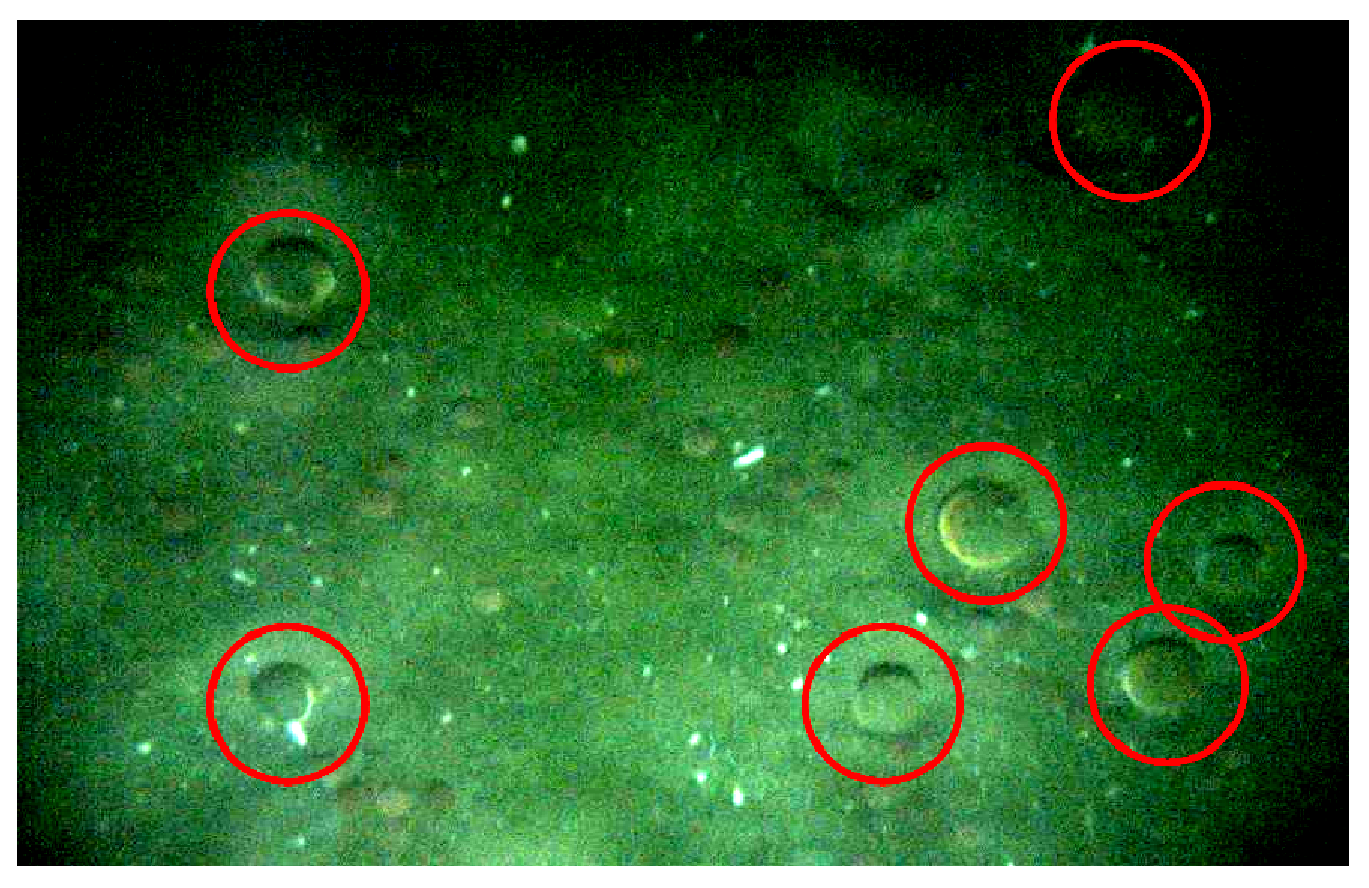
\includegraphics[width=0.6\textwidth]{scallopred}
      \caption[Seabed image with scallops shown in red circles]{Seabed image with scallops shown in red circles}
      \label{fig:scallopred}
\end{figure} 

A visual scallop population assessment process involves identifying these animals in image datasets.
A representative example of an image from the dataset we had to work with is shown in  Figure~\ref{fig:scallopred}, where the scallops are marked within red circles.
A general solution to automated image annotation might not necessarily be effective for the dataset at hand.
The need here is to identify algorithms and methods that will work best under \emph{poor} lighting and imaging conditions, characteristic of this particular scallop counting application. 
The results from using elementary image processing methods like thresholding and edge detection on the images (see Figure~\ref{subfig:thresh_scallop} and \ref{subfig:edge_scallop}) demonstrate the need for a more sophisticated approach (possibly a hybrid combination of several techniques).

\begin{figure}
  \centering
  \begin{subfigure}[]{0.15\textwidth}
      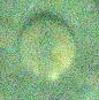
\includegraphics[width=\textwidth]{dcrescent_scallop}
      \caption{}
      \label{subfig:dcrescent_scallop}
  \end{subfigure}
  \begin{subfigure}[]{0.15\textwidth}
      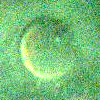
\includegraphics[width=\textwidth]{bcrescent_scallop}
      \caption{}
      \label{subfig:bcrescent_scallop}
  \end{subfigure}
  \begin{subfigure}[]{0.17\textwidth}
      \raisebox{-2pt}{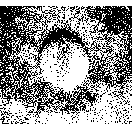
\includegraphics[width=\textwidth]{thresh}}
      \caption{}
      \label{subfig:thresh_scallop}
  \end{subfigure}
  \begin{subfigure}[]{0.17\textwidth}
      \raisebox{-2pt}{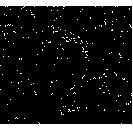
\includegraphics[width=\textwidth]{edge}}
      \caption{}
      \label{subfig:edge_scallop}
  \end{subfigure}
\caption[Scallop features]{(\subref{subfig:dcrescent_scallop}) Scallop with yellowish tinge and dark crescent; (\subref{subfig:bcrescent_scallop}) Scallop with yellowish tinge and bright shell rim crescent; (\subref{subfig:thresh_scallop}) Scallop sample after thresholding; (\subref{subfig:edge_scallop}) Scallop sample after edge detection.
}
\end{figure}

Another challenge, related to the issue of low image resolution and high levels of speckle noise, is the selection of appropriate scallop features that would enable distinguishing between these organisms and other objects. 
In the particular dataset, one recurrent visual pattern is a dark crescent on the upper perimeter of the scallop shell, which is the shadow cast by the upper open scallop shell that is produced due to the \gls{auv} strobe light (see Figure~\ref{subfig:dcrescent_scallop}). 
Another pattern that could serve as a feature in this dataset is a bright crescent on the periphery of the scallop, generally associated with the visible interior of the bottom half when the scallop shell is partly open (see Figure~\ref{subfig:bcrescent_scallop}).
A third pattern may be a yellowish tinge associated with the composition of the scallop image (see Figure~\ref{subfig:bcrescent_scallop}).

We have leveraged visual patterns \cite{prasanna_aslo} to develop a three-layered scallop counting framework  that combines tools from computer vision and machine learning. 
This particular hybrid architecture uses top-down visual attention, graph-cut segmentation and template matching along with a range of other filtering and image processing techniques. 
Though this architecture offers a performance of over 63\% true positive detection rate, it has a very large number of false positives. 
To mitigate this problem, we extend the framework \cite{prasanna_aslo} by adding a fourth, false-positives filtering layer \cite{prasanna_igi}.

%========================================================================================
\section{Scallop Survey Procedure}

The 2011 \gls{rsa} 
project (Titled: ``A Demonstration Sea Scallop Survey of the 
Federal Inshore Areas of the New York Bight using a Camera Mounted Autonomous Underwater
 Vehicle'')
was a proof-of-concept project that successfully used a digital, rapid-fire camera integrated 
to a Gavia \gls{auv}, to collect a continuous record of photographs for mosaicking, 
and subsequent scallop enumeration. 
In July 2011, transects were completed in the northwestern waters of the mid-Atlantic 
Bight at depths of 25-50 m.  The \gls{auv} continuously photographed the 
seafloor along each transect at a constant distance of 2\,m above the seafloor.  
Parallel sets of transects were spaced as close as 4\,m.  
Georeferenced images were manually analyzed for the presence of sea scallops 
using position data logged (using \gls{dvl} and \gls{ins}) with each image.
%
\subsection{Field Survey Process}
%
\begin{figure}
\centering
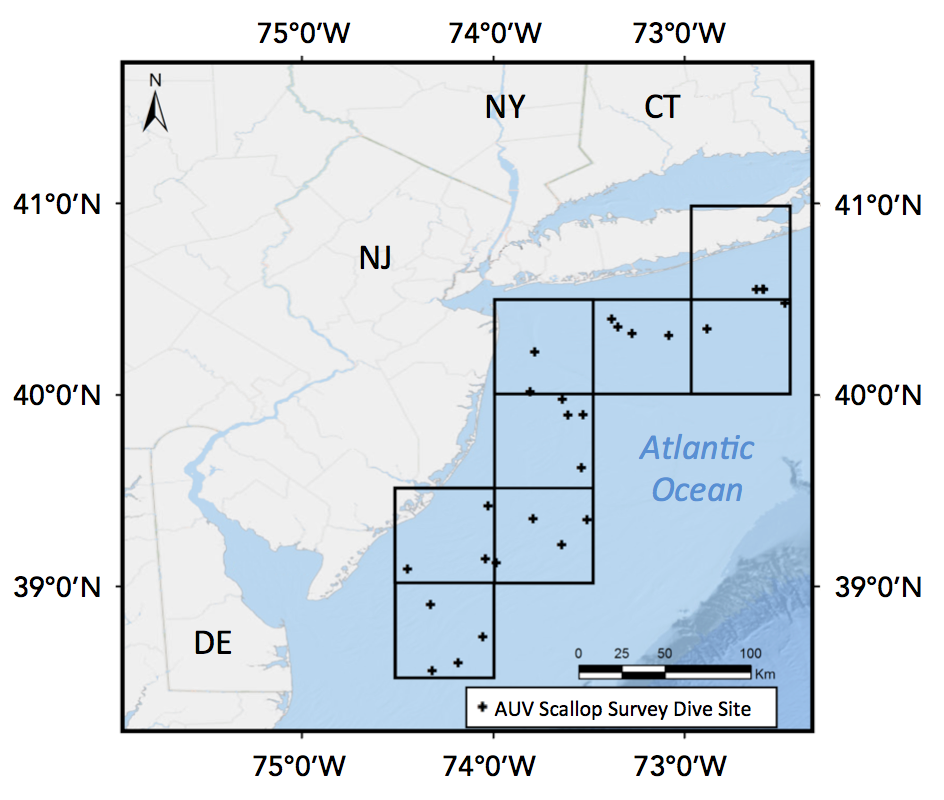
\includegraphics[width=0.5\textwidth, natwidth=944, natheight=800]{survey_region}
\caption[Map of the scallop survey region]{Map of the survey region from Shinnecock, New York to Cape May, New Jersey, 
divided into eight blocks or strata}
\label{fig:strata}
\end{figure}
%

In the 2011 demonstration survey, the federal inshore scallop grounds from Shinnecock, New York to Ocean View, Delaware, was divided into eight blocks or strata (as shown in Figure~\ref{fig:strata}).  
The \textit{f/v Christian and Alexa} served as the surface support platform 
from which a Gavia \gls{auv} (see Figure~\ref{fig:gavia_auv}) was deployed and recovered.  The \gls{auv} 
conducted photographic surveys of the seabed for a continuous duration of approximately
3 hours during each dive, repeated 3--4 times in each stratum, with
each stratum involving roughly 10 hours of imaging and an area of about $45\,000$ 
m$^2$.
The \gls{auv} collected altitude (height above the seabed) and 
attitude (heading, pitch, roll) data, allowing the georectification of each image 
into scaled images for size and counting measurements.  During the 2011 pilot study 
survey season, over $250\,000$ images of the seabed were collected. 
These images were analyzed in the University of Delaware's Coastal Sediments, Hydrodynamics and Engineering 
Laboratory for estimates of scallop
abundance and size distribution.  The \textit{f/v Christian and Alexa} provided 
surface support, and made tows along the \gls{auv} transect to ground-truth the presence of 
scallops and provide calibration for the size distribution. 
Abundance and sizing estimates were computed manually for each image using a GUI-based 
digital sizing software. 
Each image included embedded metadata that 
allowed it to be incorporated into existing benthic image classification systems
(HabCam mip \cite{dawkings13}).
% Abundance and sizing estimates were conducted via a heads-up manual method, 
% with each image including embedded metadata allowing it to be incorporated into 
% to existing benthic image classification systems (HabCam mip \citep{Dawkings13}).

During this proof of concept study, in each stratum the f/v
\textit{Christian and Alexa} made one 15-minute dredge tow along the \gls{auv} 
transect to ground-truth the presence of scallops and other fauna, 
and provide calibration for the size distribution.  The vessel was maintained 
on the dredge track by using Differential GPS.  
The tows were made with the starboard 15 ft 
(4.572\;m)
wide New Bedford style commercial dredge at the commercial dredge speed of 4.5--5.0 knots.
The dredge was equipped with 4 inch (10.16 m) interlocking rings, 
an 11 inch (27.94 cm) twine mesh top, and turtle chains.
After dredging, the catch was sorted, identified, and weighed.  
Length-frequency data were obtained for the caught scallops.  
This information was recorded onto data logs and then entered into a laptop computer database aboard ship for comparison to the camera image estimates.

The mobile platform of the \gls{auv} provided a more expansive and continuous coverage 
of the seabed compared to traditional fixed drop camera systems or towed camera systems. 
In a given day, the \gls{auv} surveys covered about $60\,000$\;m$^2$ of seabed 
from an altitude of 2\;m above the bed, simultaneously producing broad sonar 
swath coverage and measuring the salinity, temperature, dissolved oxygen, and 
chlorophyll-a  in the water.


\subsection{Sensors and Hardware}
\label{section:equipment}

The University of Delaware \gls{auv} (Figure \ref{fig:gavia_auv}) was used to collect 
continuous images of the benthos, and simultaneously map the texture and topography of 
the seabed. Sensor systems associated with this vehicle include: \begin{enumerate*}[label=(\arabic*):, start=1] 
\item a 500\;kHz GeoAcoustics GeoSwath Plus phase measuring bathymetric 
sonar; \item a 900/1800\;kHz Marine Sonic dual-frequency high-resolution 
side-scan sonar; 
\item a Teledyne Rd Instruments 1200 kHz acoustic \gls{dvl}/\gls{adcp}; 
\item a Kearfott T-24 inertial navigation system; 
\item an Ecopuck flntu combination fluorometer / turbidity sensor; 
\item a Point Grey Scorpion model 20SO digital camera and LED strobe array; 
\item an Aanderaa Optode dissolved oxygen sensor; 
\item a temperature and density sensor; and, \item an altimeter. \end{enumerate*} 
Each sensor separately records time and spatially stamped data with frequency and spacing.
The \gls{auv} is capable of very precise dynamic positioning, adjusting to the variable 
topography of the seabed while maintaining a constant commanded altitude offset.

\begin{figure}
  \centering
  \begin{subfigure}[]{0.7\textwidth}
      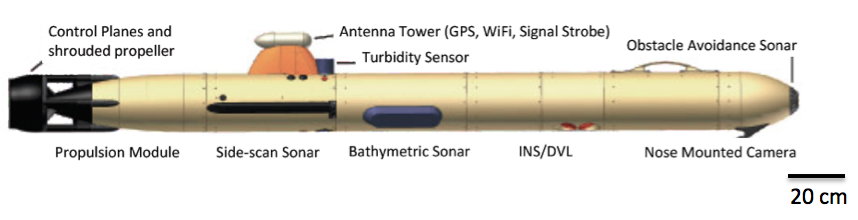
\includegraphics[width=\textwidth,natwidth=1052,natheight=428]{auv_schematics}
  \end{subfigure}
  \begin{subfigure}[]{0.6\textwidth}
      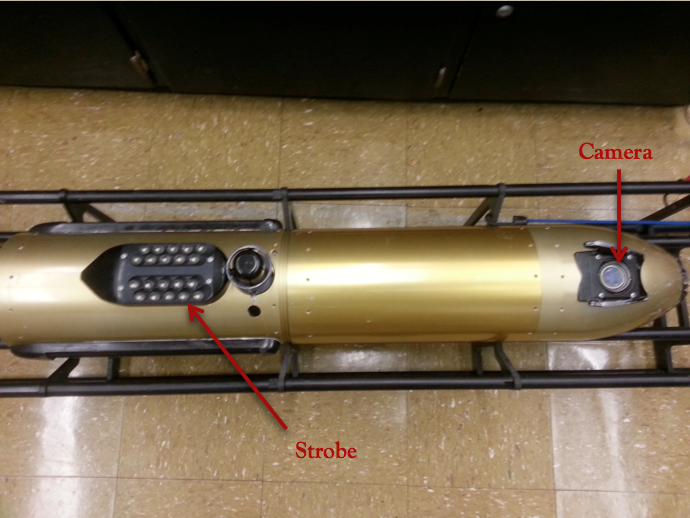
\includegraphics[width=\textwidth,natwidth=690,natheight=518]{auv_image}    
  \end{subfigure}
  \caption{Schematics and image of the Gavia \gls{auv} }
  \label{fig:gavia_auv}
\end{figure}

\subsection{Data Collection}

The data was collected over two separate five-day cruises in July 2011.   
In total, 27 missions were run using the \gls{auv} to photograph the seafloor (For list of missions see Table \ref{tab:mission_list}).  
Mission lengths were constrained by the 2.5 to 3.5 hour battery life of the \gls{auv}.  
During each mission, the \gls{auv} was instructed to follow a constant height of 2\;m
above the seafloor.  In addition to the $250\,000$ images that were collected, the 
\gls{auv} also gathered data about water temperature, salinity, dissolved oxygen, 
geoswath bathymetry, and side-scan sonar of the seafloor.

The camera on the \gls{auv}, a Point Grey Scorpion model 20SO (for camera specifications see Table \ref{tab:camera_specs}), 
was mounted inside the nose module of the vehicle.
It was focused at 2\;m, and captured
images at a resolution of $800\times600$.  The camera lens had a horizontal viewing 
angle of 44.65 degrees.  Given the viewing angle and distance from the seafloor, 
the image footprint can be calculated as $1.86\times1.40$\;m$^2$.
Each image was saved in jpeg format, with metadata that included position information 
(including latitude, longitude, depth, altitude, pitch, heading and roll)  
and the near-seafloor environmental conditions analyzed in this study.  
This information is stored in the header file, making the images readily comparable and 
ready to be incorporated into existing \gls{rsa} image databases, such as the 
HabCam database.
A manual count of the number of scallops in each image was performed and used to obtain overall scallop
abundance assessment.
Scallops counted were articulated shells in life position (left valve up) \cite{walker}.
%
\begin{table}
\centering
\begin{threeparttable}
      \begin{tabular}{ll}
      \toprule[1pt]\\[-6pt]
      Mission  & Number of images\\[2pt]\midrule
      LI1\tnote{1}	&$12\,775$\\
      LI2	&$2\,387$\\
      LI3	&$8\,065$\\
      LI4	&$9\,992$\\
      LI5	&$8\,338$\\
      LI6	&$11\,329$\\
      LI7	&$10\,163$\\
      LI8	&$9\,780$\\
      LI9	&$2\,686$\\
      NYB1\tnote{2}	&$9\,141$\\
      NYB2	&$9\,523$\\
      NYB3	&$9\,544$\\
      NYB4	&$9\,074$\\
      NYB5	&$9\,425$\\
      NYB6	&$9\,281$\\
      NYB7	&$12\,068$\\
      NYB8	&$9\,527$\\
      NYB9	&$10\,950$\\
      NYB10	&$9\,170$\\
      NYB11	&$10\,391$\\
      NYB12	&$7\,345$\\
      NYB13	&$6\,285$\\
      NYB14	&$9\,437$\\
      NYB15	&$11\,097$\\
      ET1\tnote{3}	&$9\,255$\\
      ET2	&$12\,035$\\
      ET3	&$10\,474$\\
      \\[2pt]\bottomrule[1pt]
    \end{tabular}
    \begin{tablenotes}
       \vskip 5pt
	  \item[1] \footnotesize{LI--Long Island}
	  \item[2] \footnotesize{NYB--New York Bight}
	  \item[3] \footnotesize{ET--Elephant Trunk}
      \end{tablenotes}                                                      
 \end{threeparttable}
  \caption{List of missions and number of images collected}
  \label{tab:mission_list}
\end{table}

%                                                      
\begin{table}                                                     
\centering
\begin{tabularx}{\textwidth}{XX}
\toprule[1pt]\\[-6pt]
Attribute	&Specs\\[2pt]\midrule
Name	&Point Grey Scorpion 20SO Low Light Research Camera\\
Image Sensor	&8.923 mm Sony ccd\\
Horizontal Viewing Angle	&44.65 degrees (underwater)\\
Mass	&125 g\\
Frame rate	&3.75 fps\\
Memory	&Computer housed in \gls{auv} nose cone\\
Image Resolution	&800 $\times$ 600\\
Georeferenced metadata	&Latitude, longitude, altitude, depth\\
Image Format	&jpeg\\[2pt]\bottomrule[1pt]
\end{tabularx}
\caption{Camera specifications\label{tab:camera_specs}}
\end{table}


%========================================================================================
\section{Methodology}

The multi-layered scallop counting framework that comprises four layers of processing on underwater images for the purpose of obtaining scallop counts is discussed in this section. 
The four layers involve the sequential application of Top-Down Visual Attention, Segmentation, Classification and False-Positive Filtering.

\subsection{Layer I: Top-Down Visual Attention} \label{subsec:TDVA}

\subsubsection{Learning}

A customized \gls{tdva} algorithm can be designed 
to sift automatically through the body of imagery data, and focus on
regions of interest that are more likely to contain scallops.
The process of designing the \gls{tdva} algorithm is described below.

The first step is a small-scale, \gls{buva} based saliency computation. 
The saliency computation is performed 
on a collection of randomly selected 243 annotated images, collectively containing 300 scallops.
This collection constitutes the \emph{learning set}.
Figure~\ref{fig:saliency_combine} represents graphically the flow of computation
and shows the type of information in a typical image that visual attention tends to highlight.
%
\begin{figure*}
\vskip -5pt
\centering
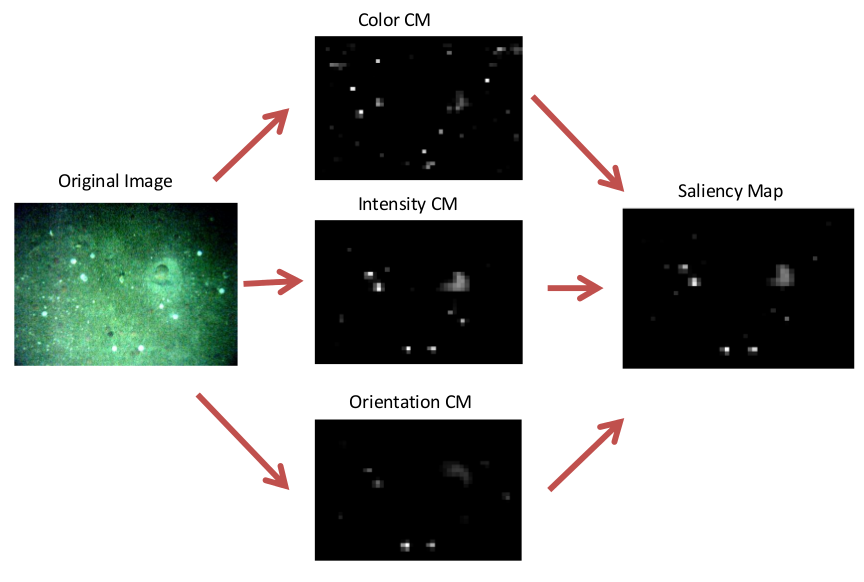
\includegraphics[width=0.80\textwidth,natwidth=864,natheight=582]{saliency_example1.png}
\caption{Illustration of computation flow for the construction of saliency maps}
\label{fig:saliency_combine}
\end{figure*}
%

A process of extremum
seeking on the saliency map of each image identifies fixations in the associated image.
If a $100\times100$ pixel window---corresponding to an approximately $23 \times 23$\enspace cm$^2$ area on the seafloor---centered around a fixation point
contained the center of a scallop, the corresponding 
fixation was labeled a \emph{target}; otherwise, it is considered a \emph{distractor}.

\begin{figure} 
% \vskip +6pt
\centering
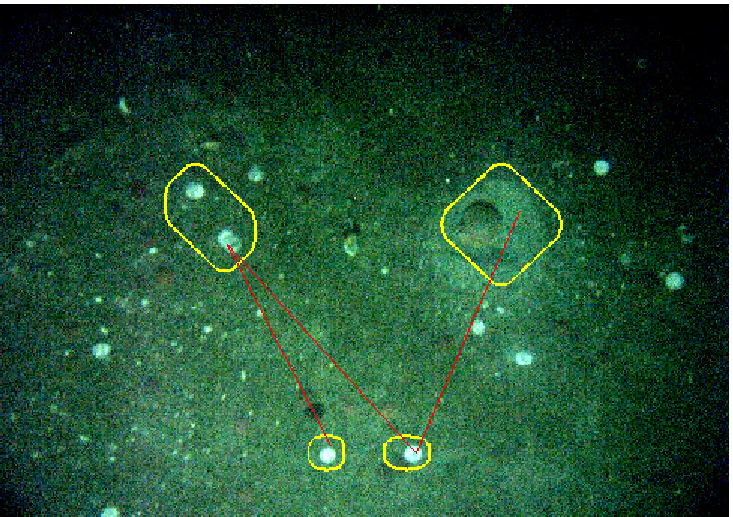
\includegraphics[width=0.6\textwidth,natwidth=800,natheight=600]{fixation_example.pdf}
\caption[Illustration of fixations]{Illustration of fixations (marked by yellow boundaries):
         red lines indicate the order in which the fixations were detected with the lower-left fixation being the first.
}
\label{fig:fixation}
%\vskip -15pt
\end{figure}

The target and distractor regions are determined in all the feature and conspicuity maps for each one of these processed images in the learning set.
This is done by adaptively thresholding and locally segmenting the points around the fixations with similar salience values in each map.
Then the mean numerical value in neighborhoods around  
these target and distractor regions in the feature maps and conspicuity maps 
are computed.  These values are used to populate the $P_{ijT_k}$ and $P_{ijD_r}$ variables in \eqref{eq:learning_wts_all}, and determine the top-down weights for feature maps and conspicuity maps.

For the conspicuity maps, the center-surround scale weights $w_{cs}$ computed through \eqref{eq:learning_wts_all} and consequently used in \eqref{eq:feature_map},
are shown in Table \ref{tab:tdva_fm_wts}.
For the saliency map computation, the weights resulting from the application of
\eqref{eq:learning_wts_all} on the conspicuity maps are
$w_{\bar{I}}= 1.1644$, $w_{\bar{C}}= 1.4354$ and $w_{\bar{O}}= 0.4001$.  
The symmetry of the scallop shell in our low-resolution dataset 
justifies the relatively small value of the orientation weight.

\begin{table*}
\caption{Top-down weights for feature maps \label{tab:tdva_fm_wts}}
\centering
\begin{tabular}{llllllll}
\toprule[1pt]\\[-6pt]
 &   & \multicolumn{6}{c}{Center Surround Feature Scales}\\[2pt]\cline{1-8}\\[-5pt]
  &   & 1 & 2 & 3 & 4 & 5 & 6\\[2pt]\cline{1-8}\\[-5pt]
Color & red-green & 0.8191 & 0.8031 & 0.9184 & 0.8213 & 0.8696 & 0.7076\\
  & blue-yellow & 1.1312 & 1.1369 & 1.3266 & 1.2030 & 1.2833 & 0.9799\\[8pt]
Intensity & intensity & 0.7485 & 0.8009 & 0.9063 & 1.0765 & 1.3111 & 1.1567\\[8pt]
Orientation & $0^\circ$ & 0.7408 & 0.2448 & 0.2410 & 0.2788 & 0.3767 & 2.6826\\
  & $45^\circ$ & 0.7379 & 0.4046 & 0.4767 & 0.3910 & 0.7125 & 2.2325\\
  & $90^\circ$ & 0.6184 & 0.5957 & 0.5406 & 1.2027 & 2.0312 & 2.1879\\
  & $135^\circ$ & 0.8041 & 0.6036 & 0.7420 & 1.5624 & 1.1956 & 2.3958\\[2pt]\bottomrule[1pt]
\end{tabular}
\end{table*}
% 

                                                   

\subsubsection{Implementation and Testing}\label{sec:tdva-testing}

To test the performance of the customized \gls{tdva} algorithm, it is applied on
two image datasets, the size of which is shown in Table~\ref{tab:count_results}.
In this application, the saliency maps are computed via the formulae 
\eqref{eq:saliency_map} and \eqref{eq:feature_map},
using the weights listed in Table \ref{tab:tdva_fm_wts}.
Convergence time of the winner-takes-all neural network that finds fixations in the saliency map of each image in the datasets of Table~\ref{tab:count_results}, is controlled using dynamic thresholding:
It is highly unlikely that a fixation that contains an object of interest
requires more than $10\,000$ iterations. If convergence to some fixation takes 
more than this number of iterations, 
then the search is terminated and no more fixations
are sought in the image.

Given that an image in datasets of
Table~\ref{tab:count_results} contains two scallops on average, no more than
ten fixations are sought in each image (The percentage of images
in the datasets that contained more than $10$ scallops 
was $0.002\%$).
Since in the testing phase the whole scallop---not just the center---needs to be included in the fixation window, the size of this window is set at
$270\times270$ pixels; more than $91$\% of the scallops are accommodated inside the window (Figure~\ref{fig:window_length}). 

\begin{figure}
  \centering
  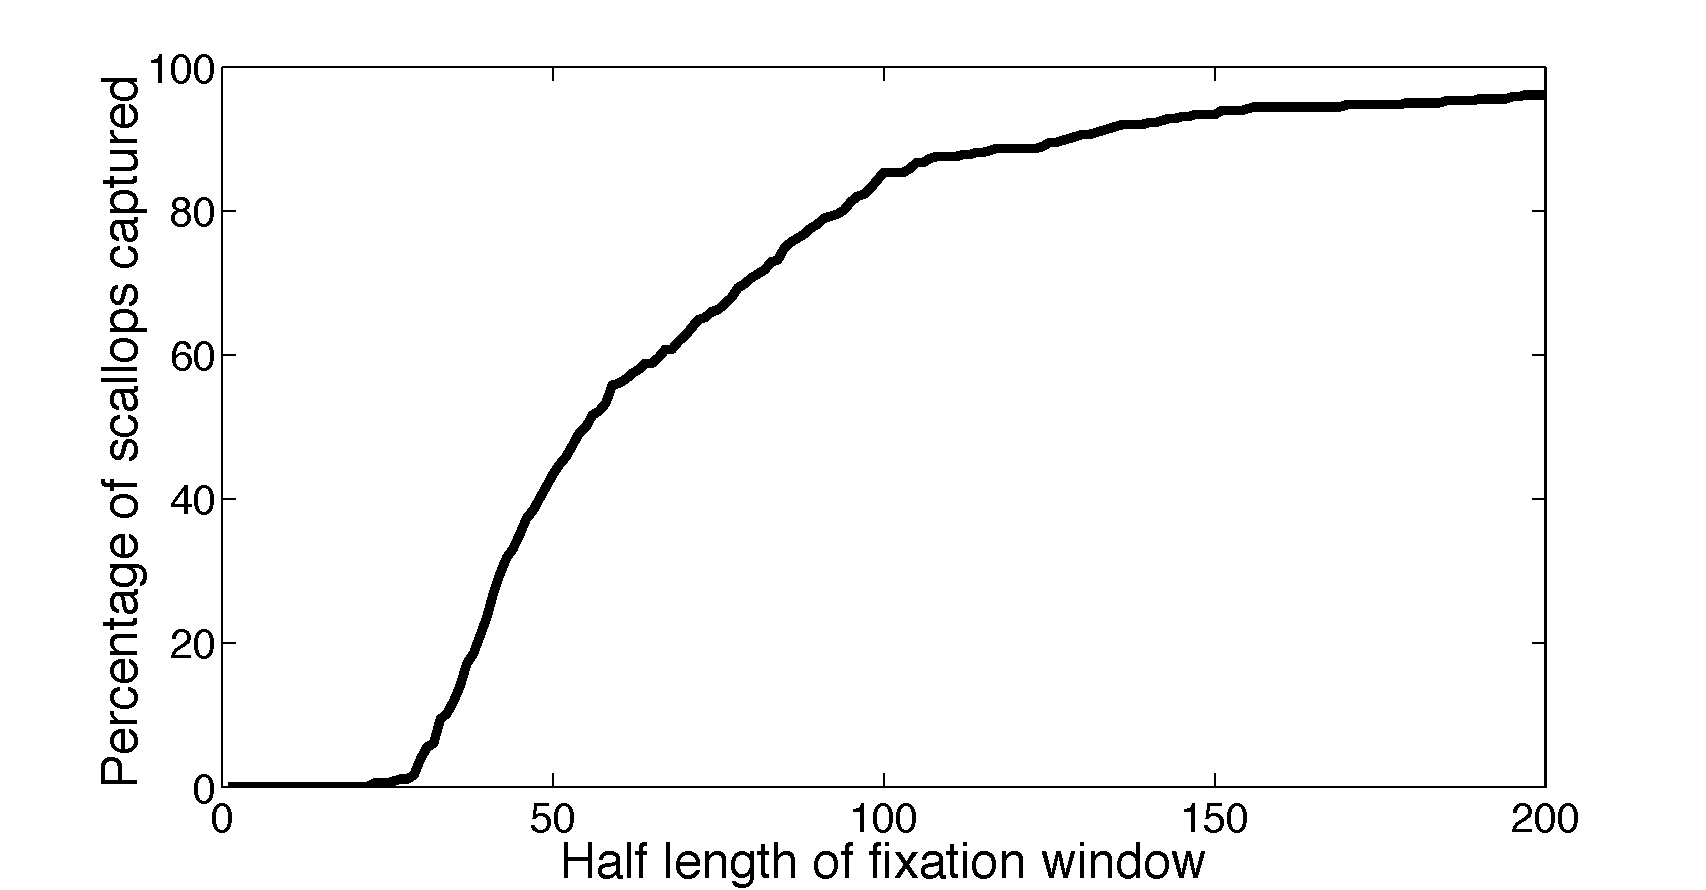
\includegraphics[width=0.60\textwidth,natwidth=800,natheight=600]{windowlength.pdf}
  \caption[Scallop fixation window dimension analysis]{Percentage of scallops enclosed in the fixation window as a function of
  window half length (in pixels)}
  \label{fig:window_length}
\end{figure}

\begin{figure*}
  \centering
  \begin{subfigure}[]{0.17\textwidth}
      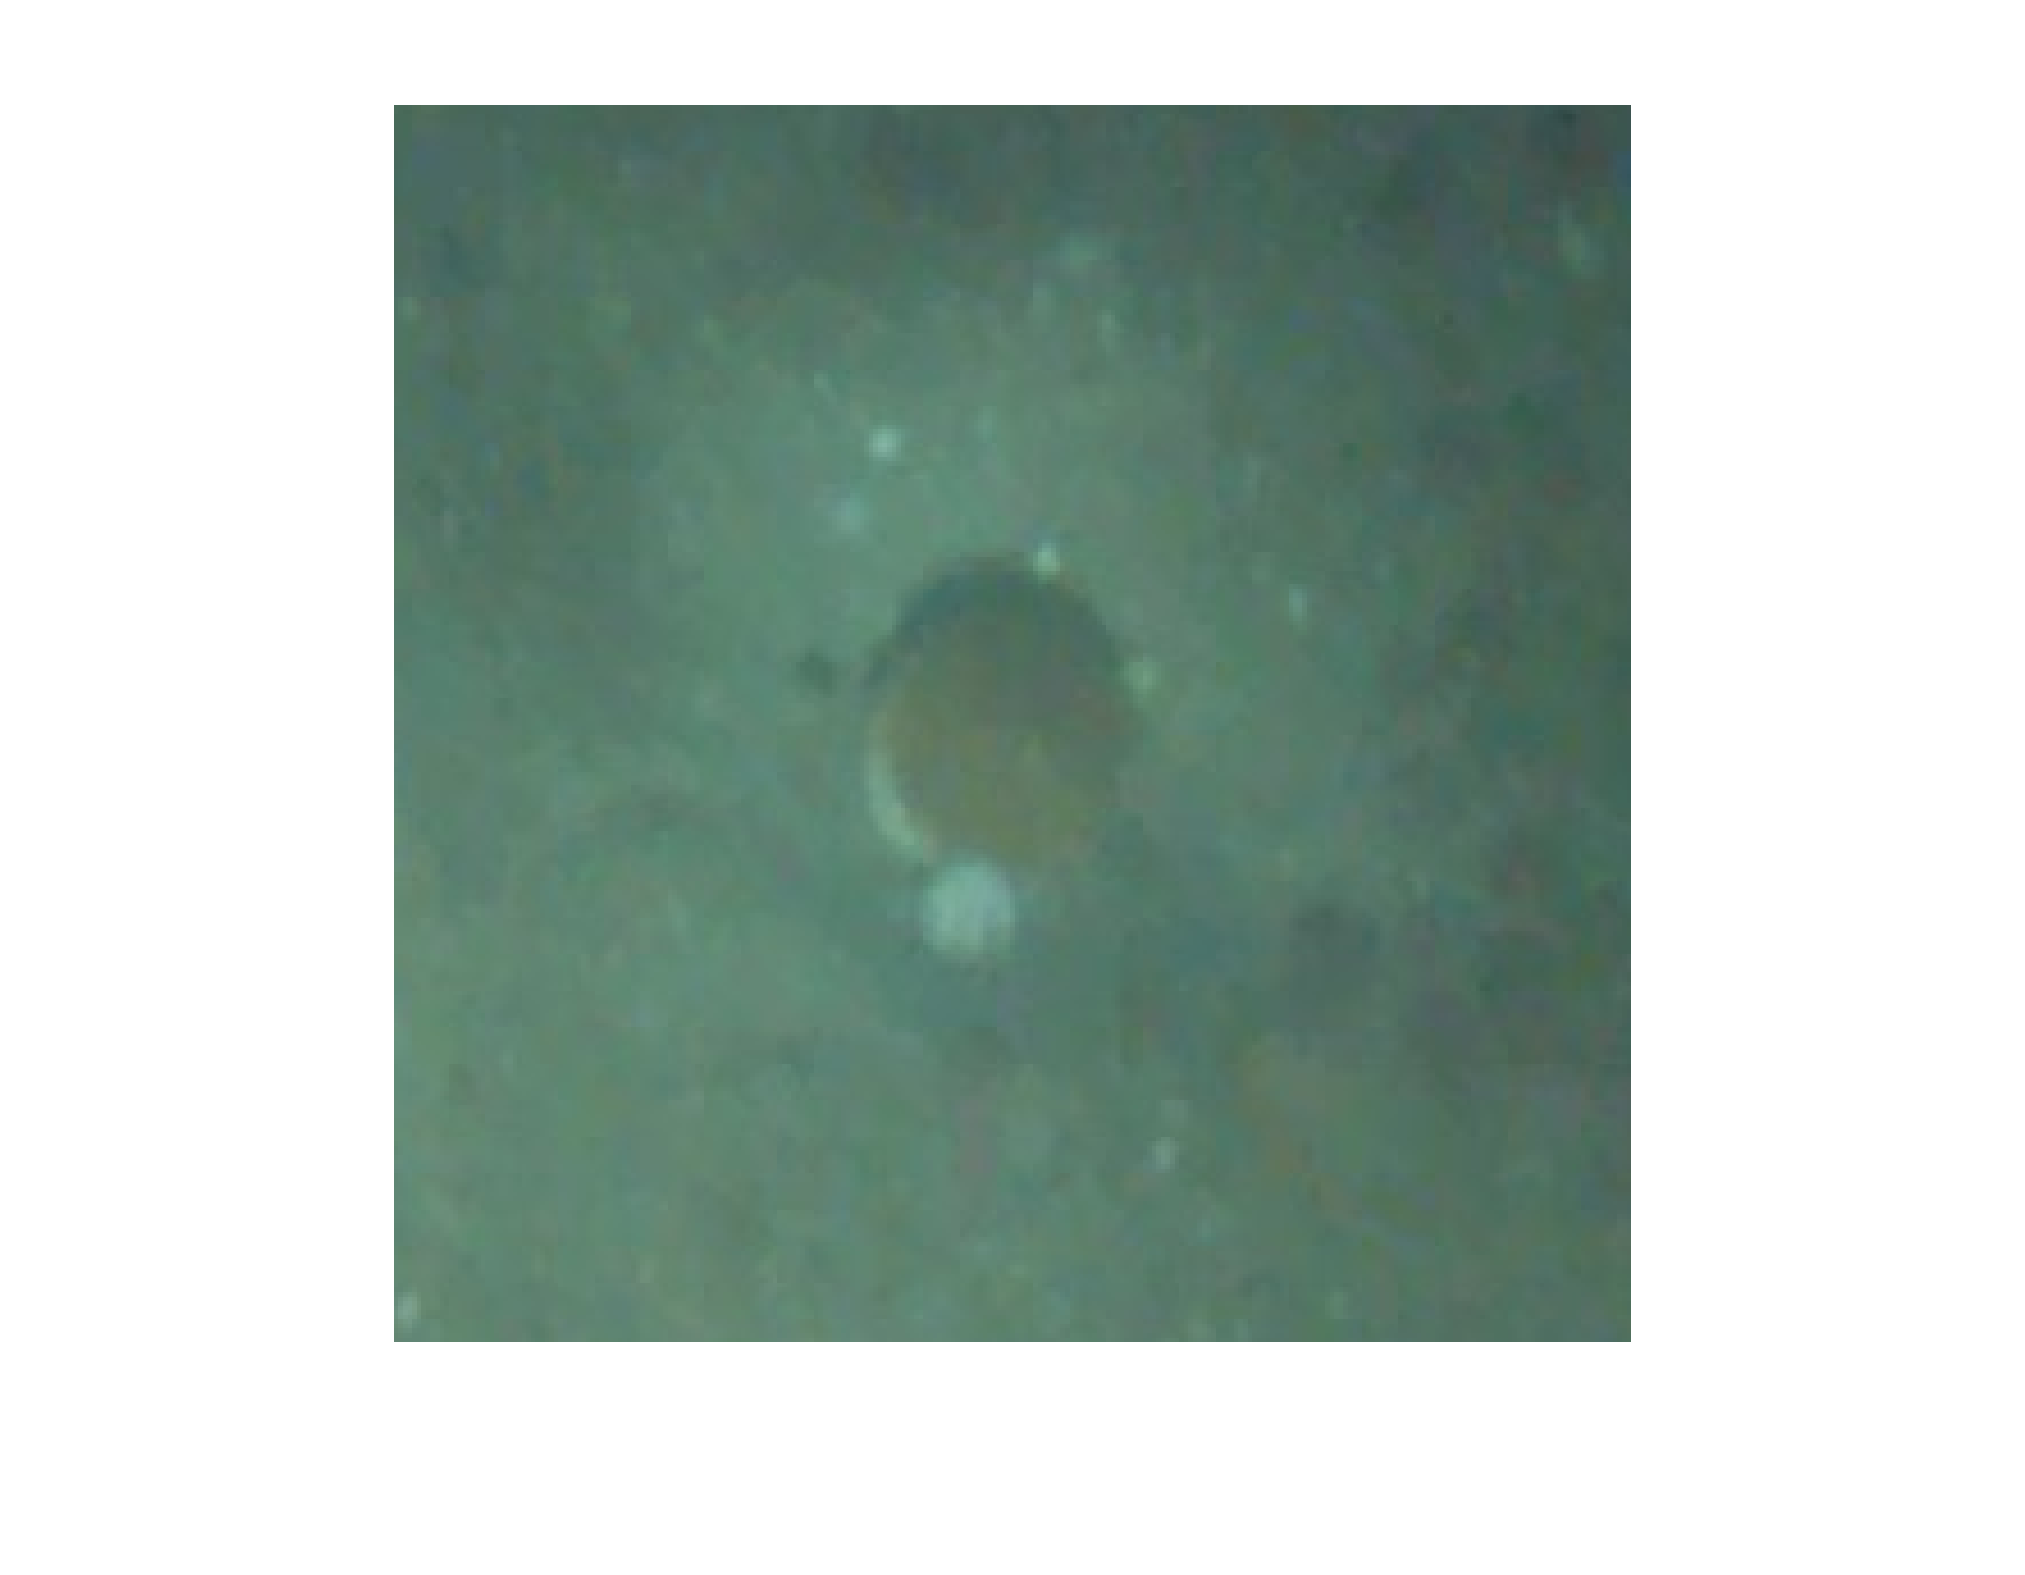
\includegraphics[width=\textwidth,natwidth=842,natheight=844]{fixationwindow.pdf}
      \caption{}
      \label{subfig:fixationwindow}
  \end{subfigure}
  \begin{subfigure}[]{0.17\textwidth}
      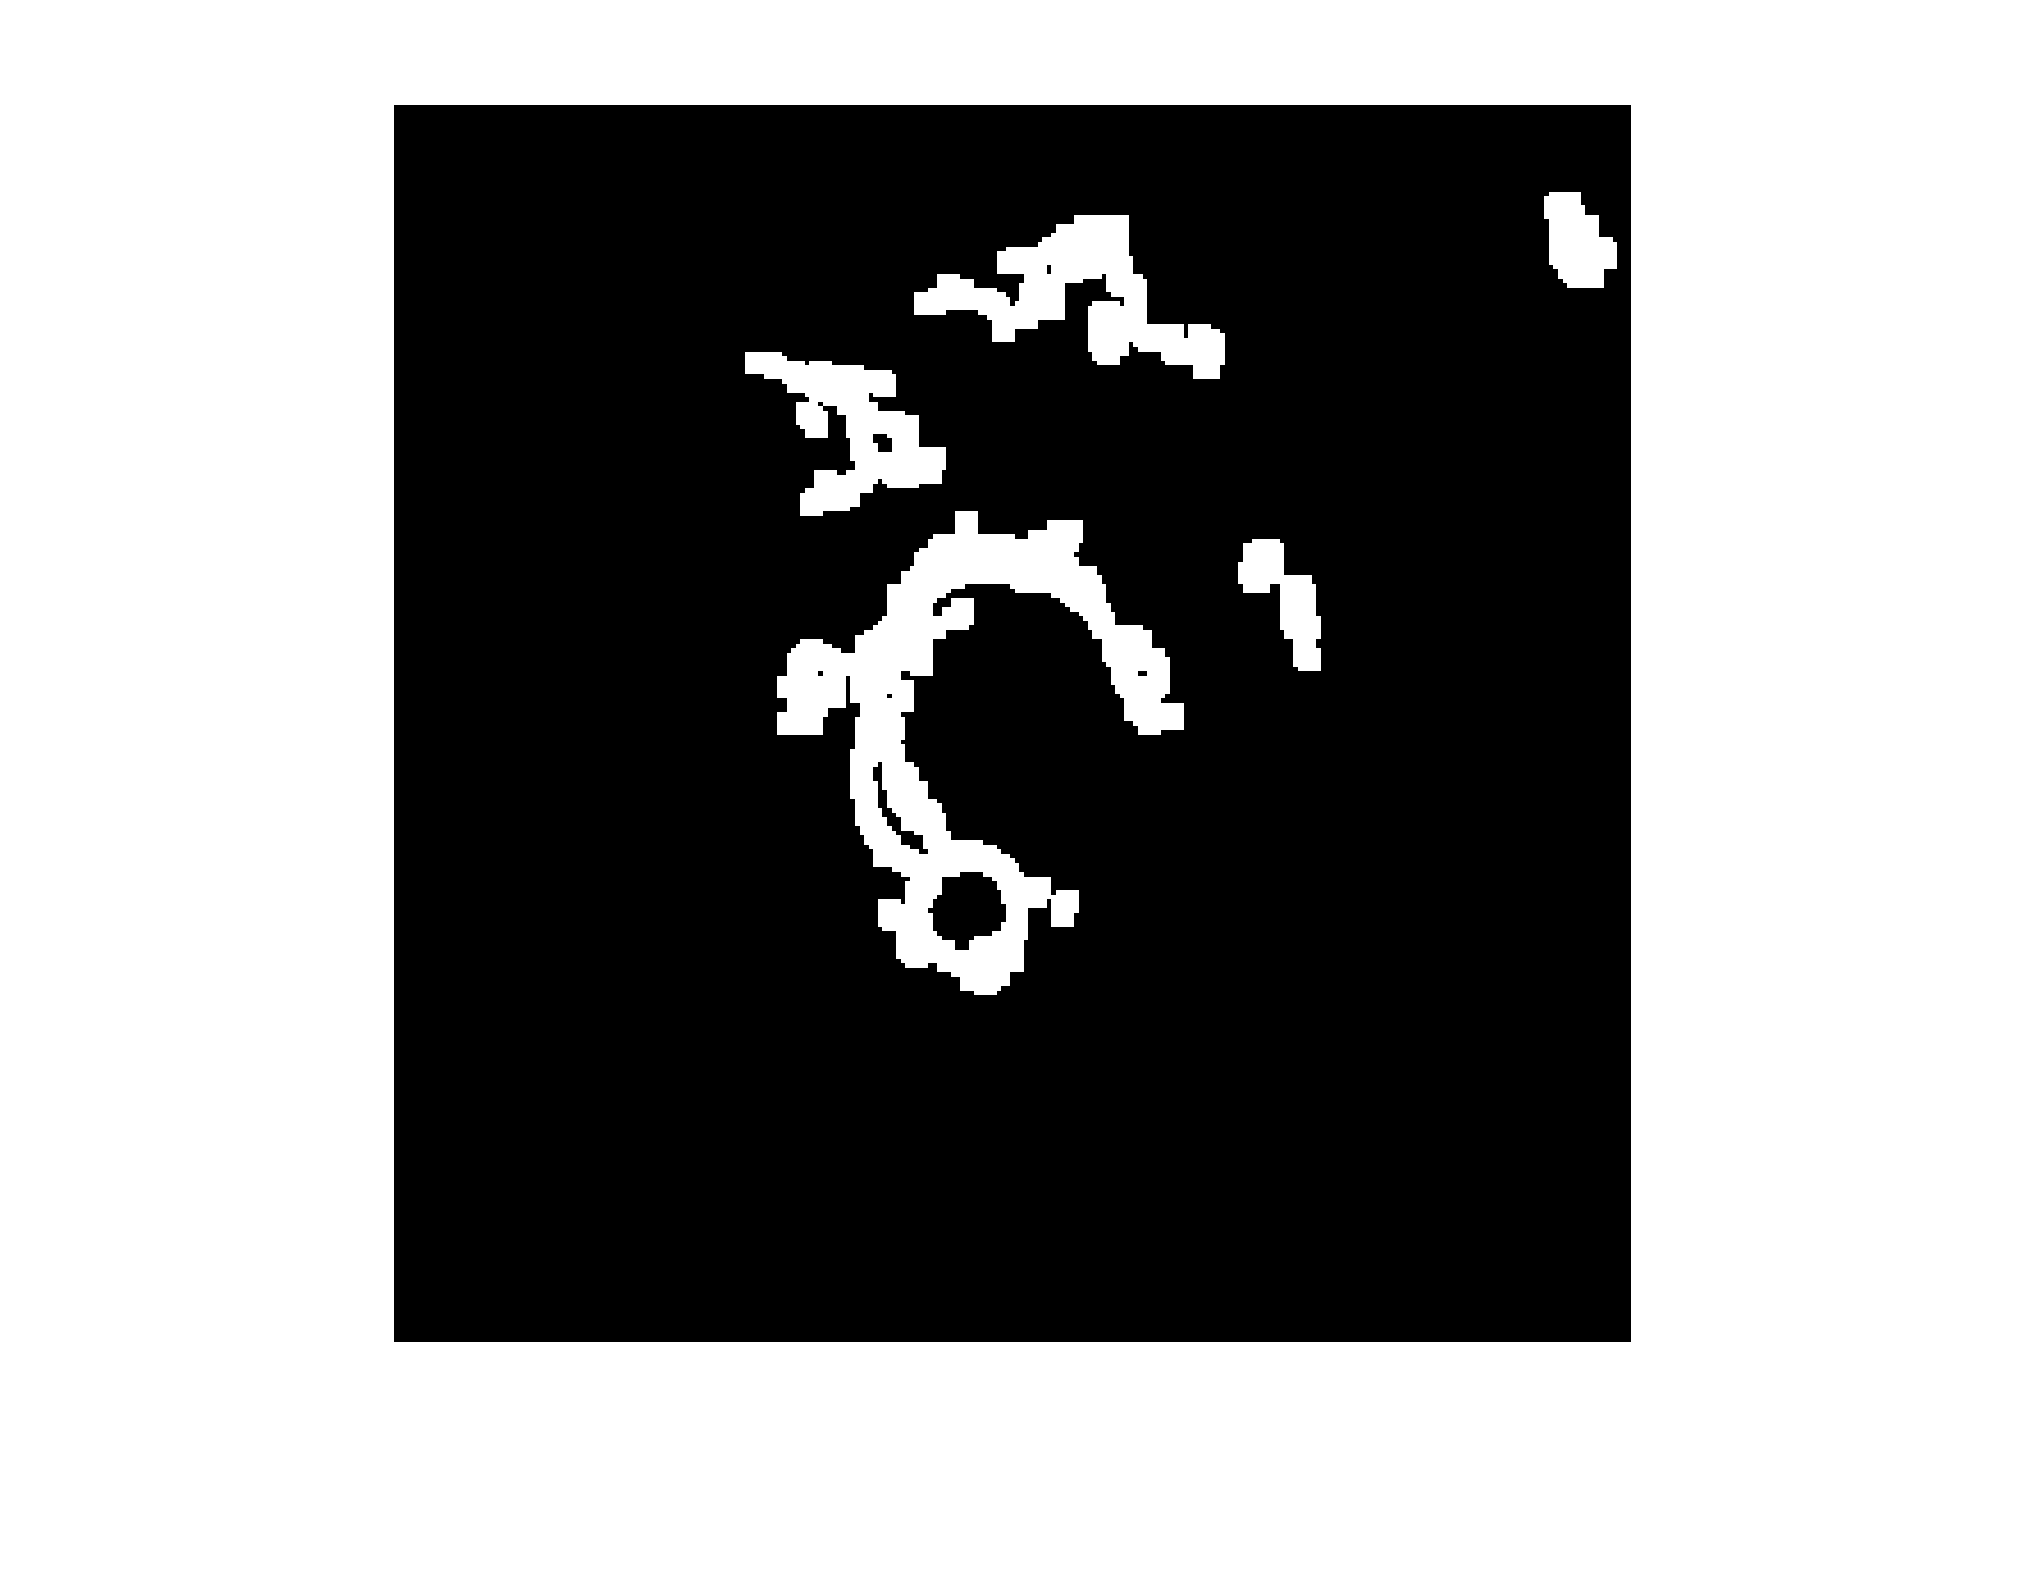
\includegraphics[width=\textwidth,natwidth=837,natheight=839]{edgeimg.pdf}
      \caption{}
      \label{subfig:edgeimg}
  \end{subfigure}
  \begin{subfigure}[]{0.17\textwidth}
      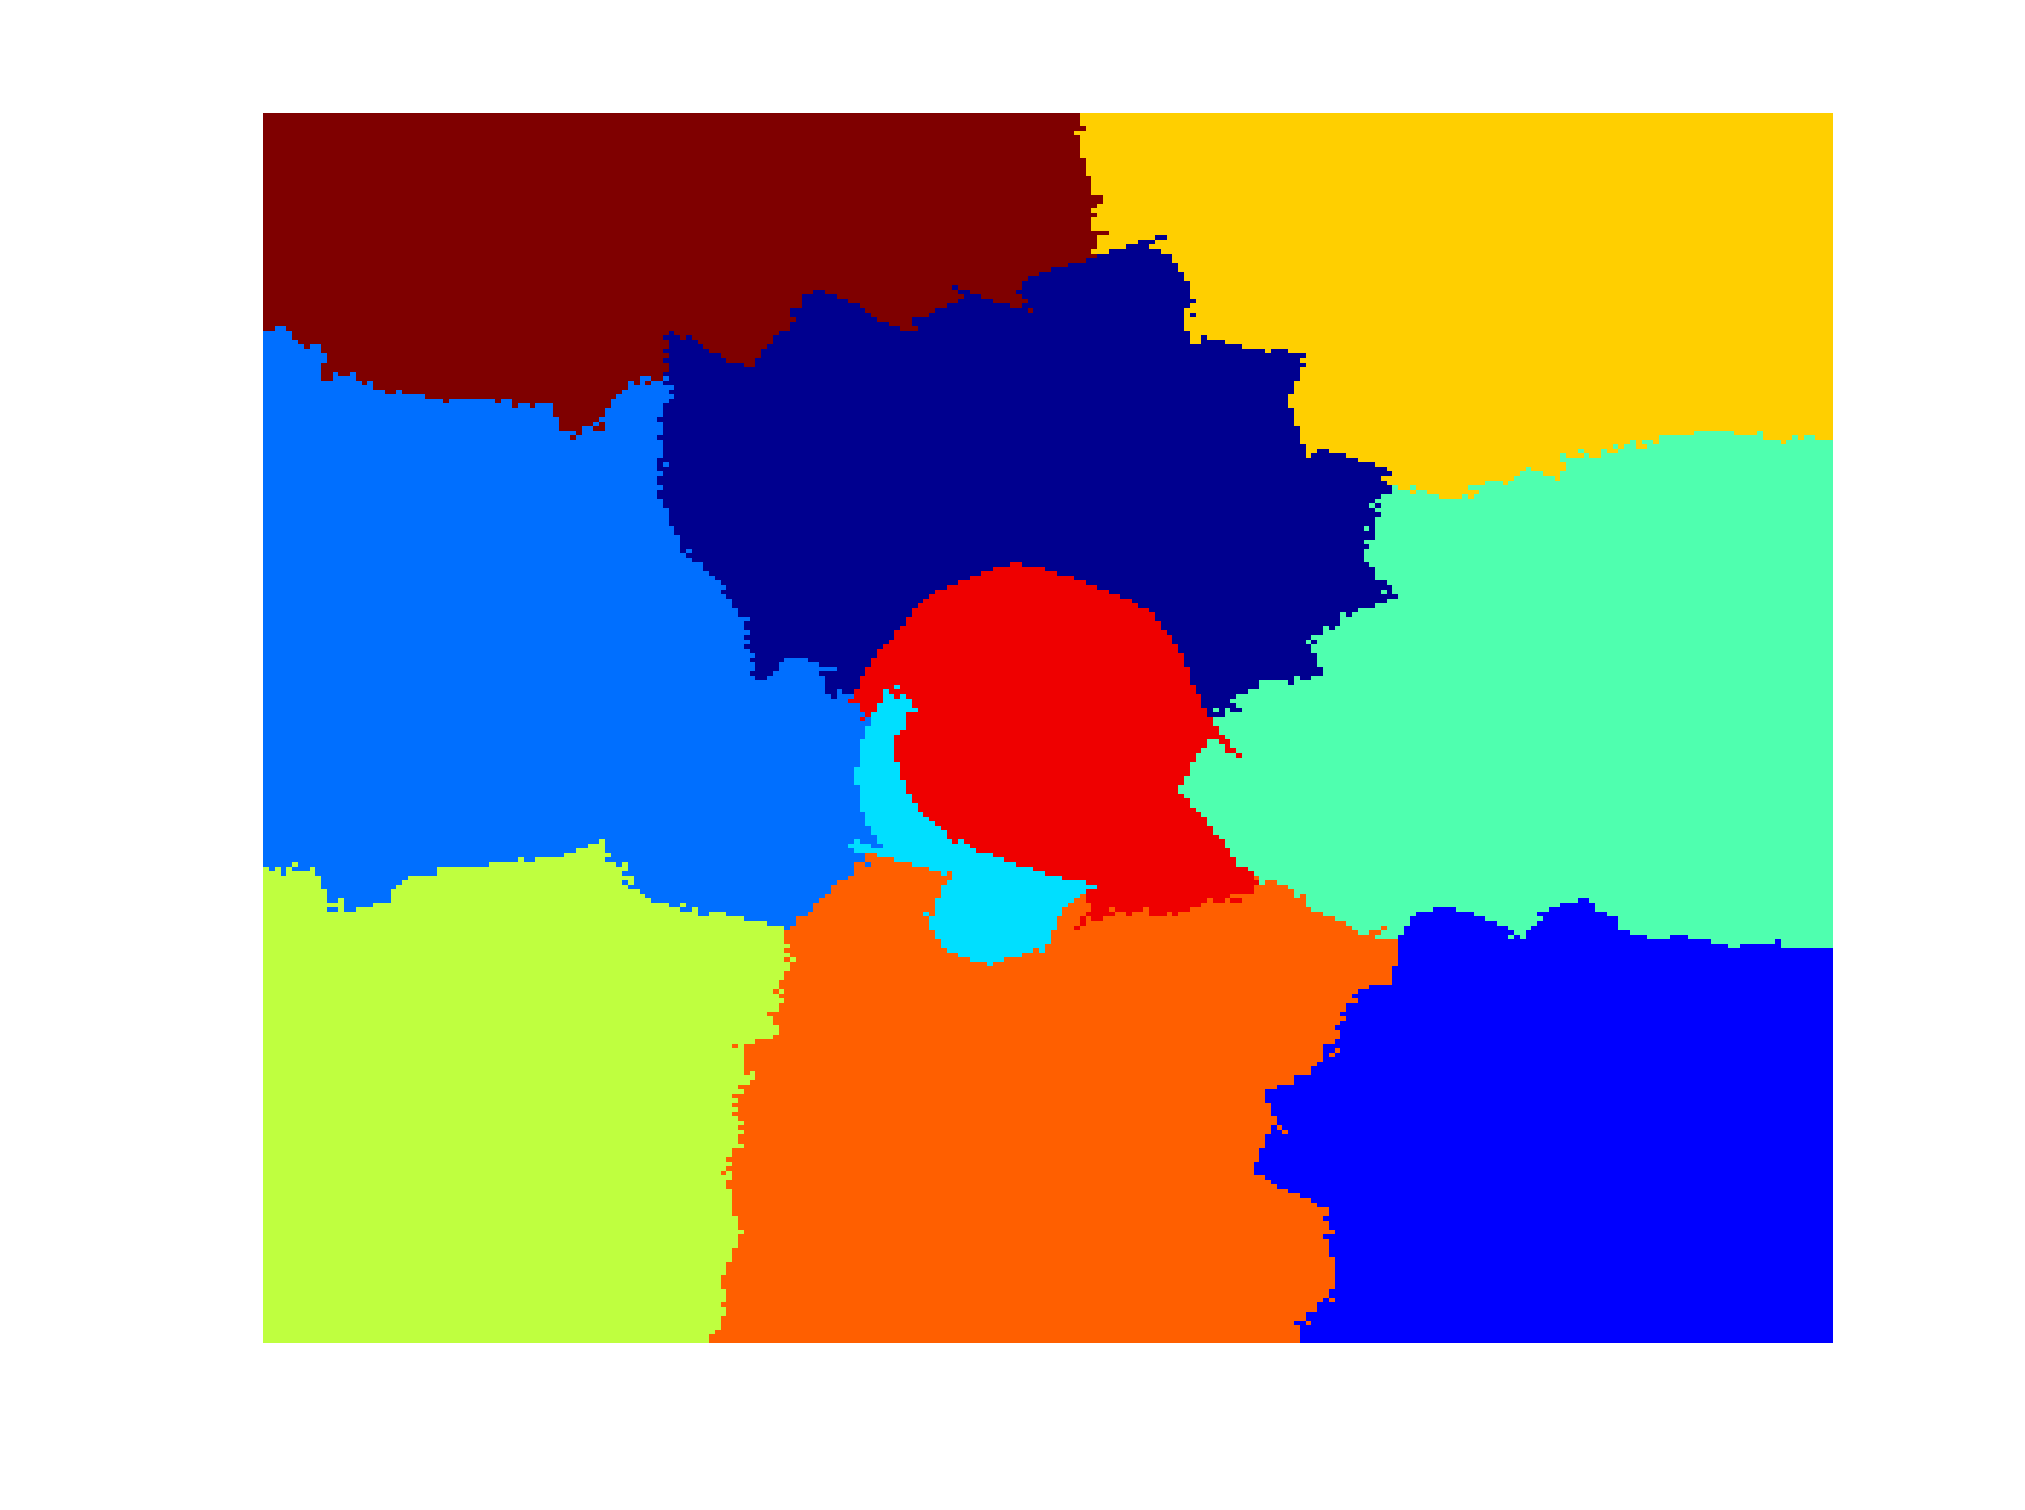
\includegraphics[width=\textwidth,natwidth=1055,natheight=842]{graphimg.pdf}    
      \caption{}
      \label{subfig:graphimg}
  \end{subfigure}
  \begin{subfigure}[]{0.17\textwidth}
      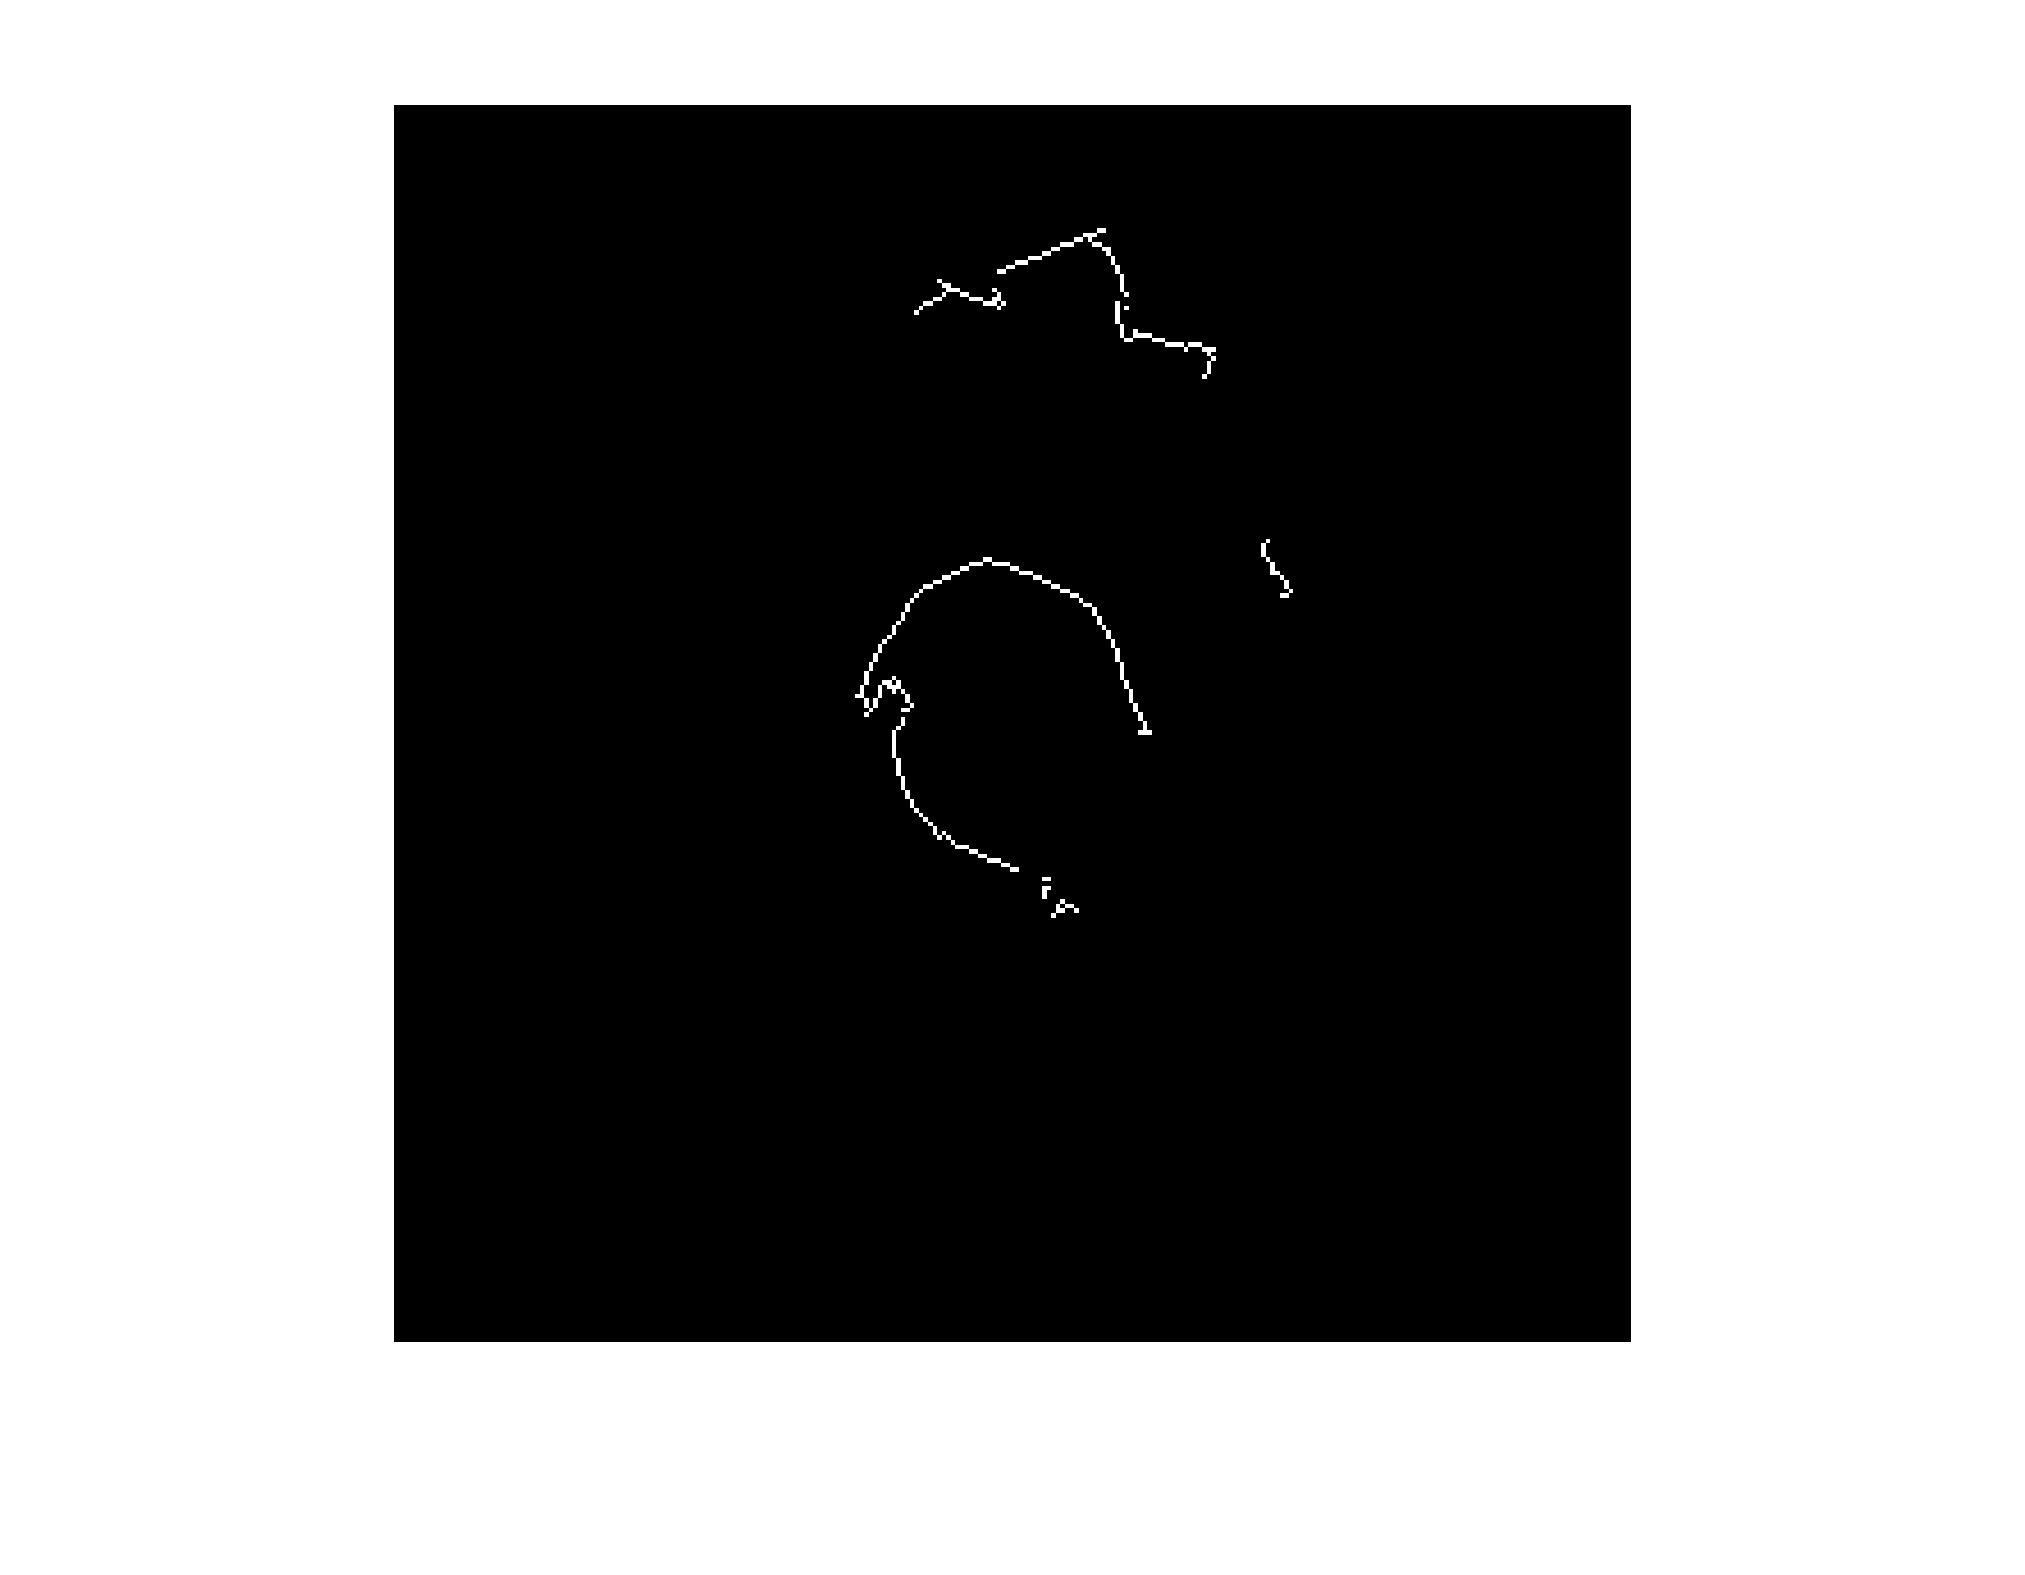
\includegraphics[width=\textwidth,natwidth=834,natheight=837]{regboundry.pdf}
      \caption{}
      \label{subfig:regboundry}
  \end{subfigure}
  \begin{subfigure}[]{0.17\textwidth}
      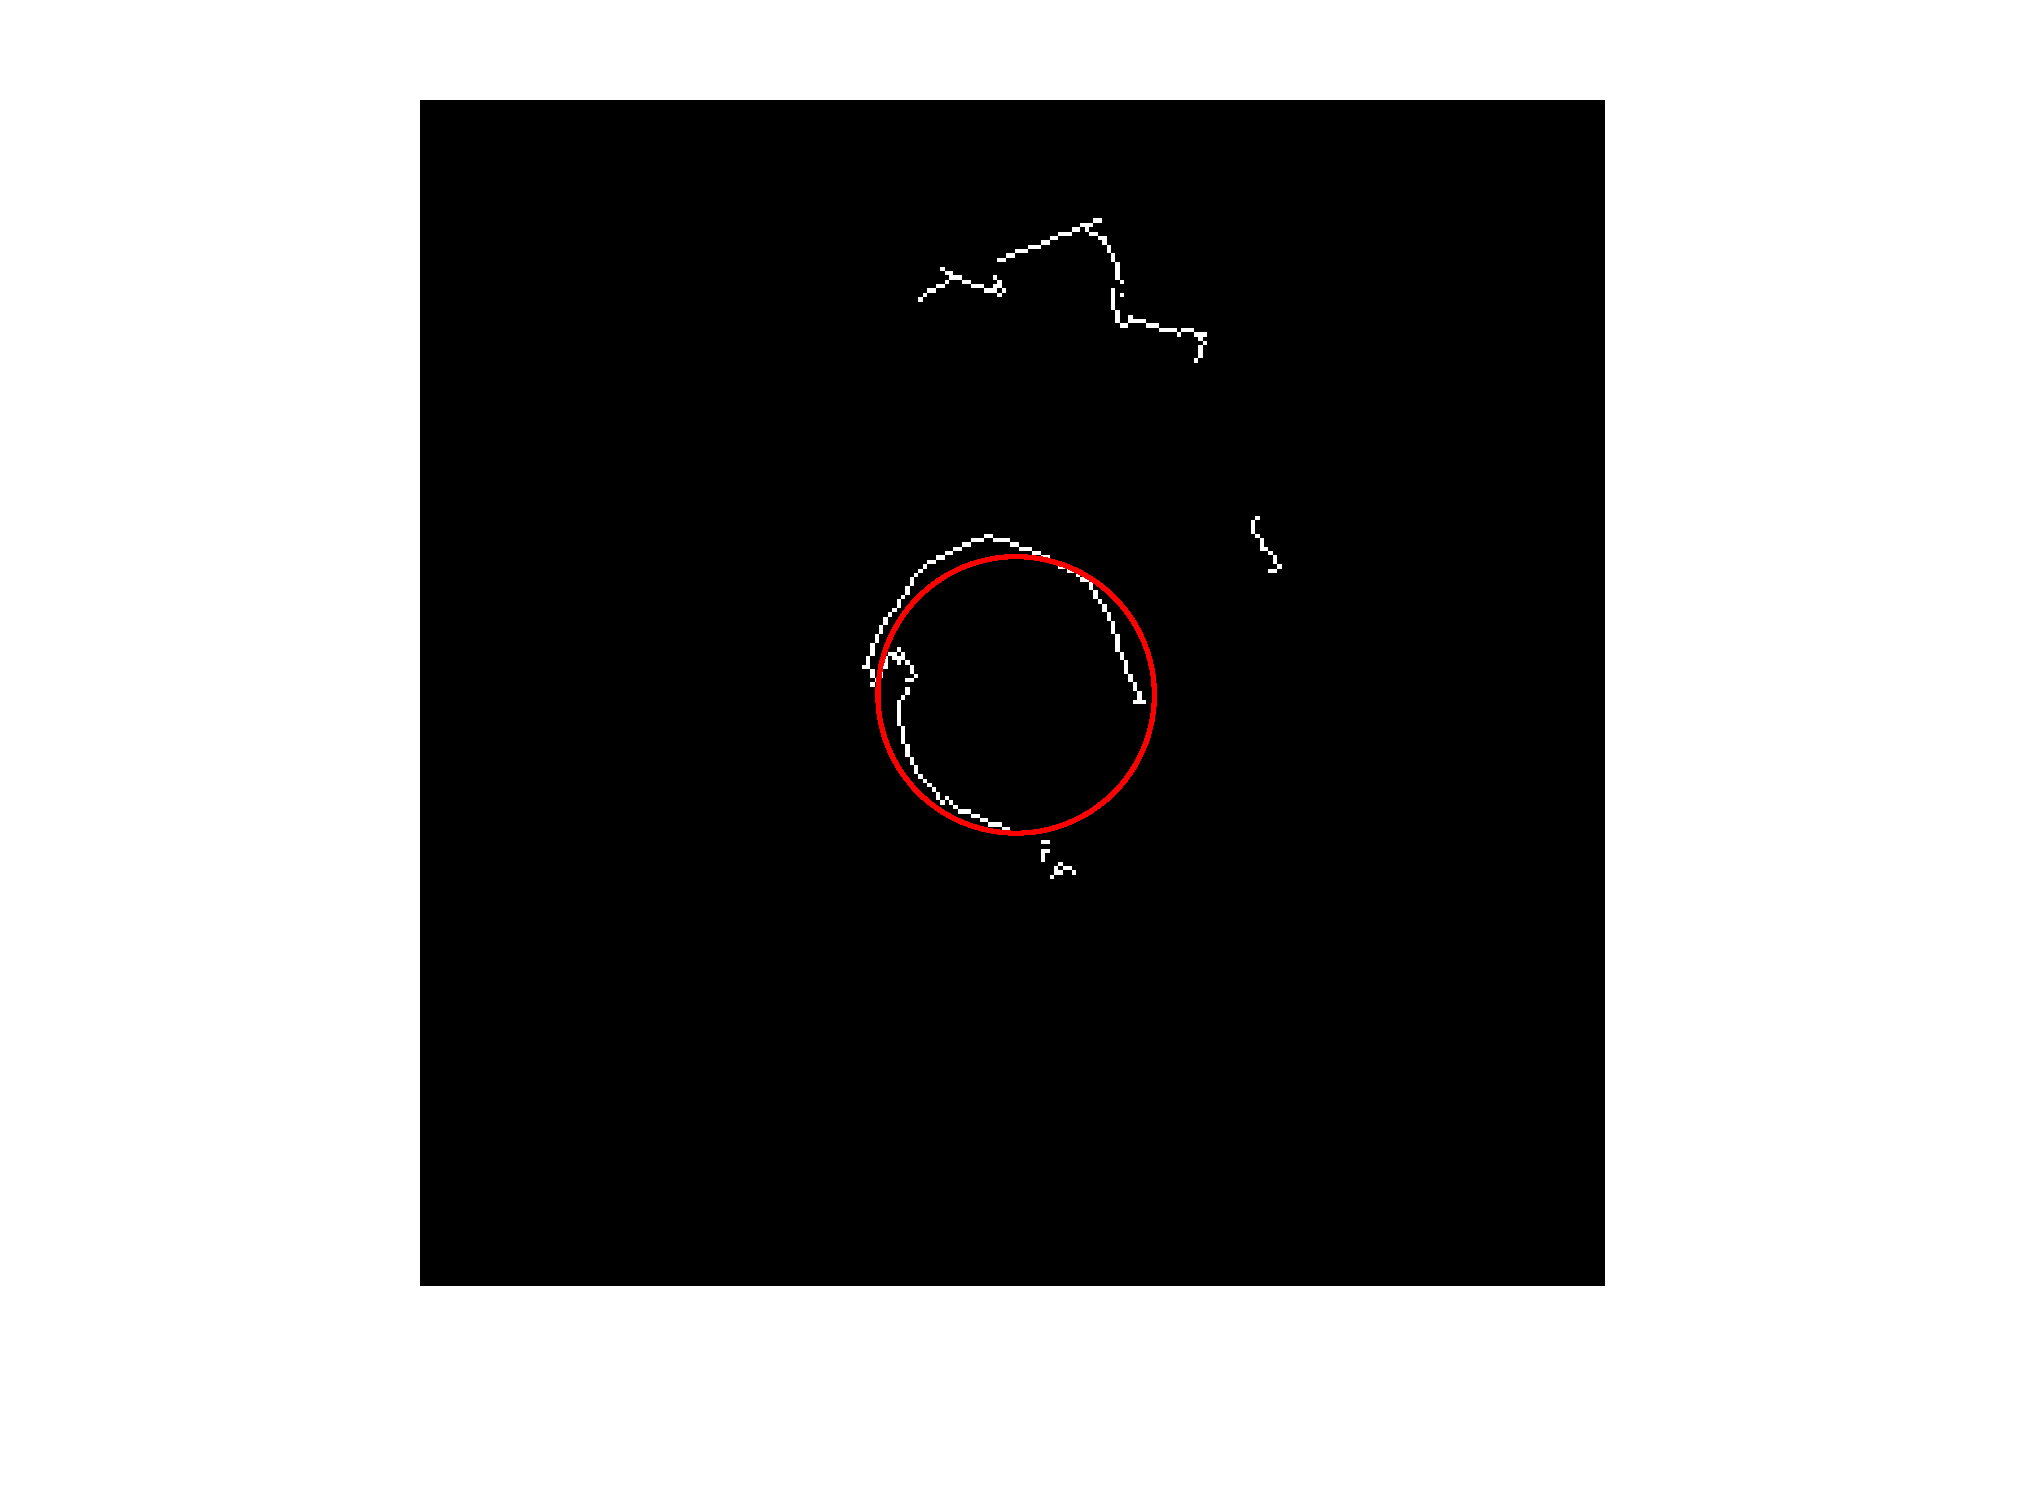
\includegraphics[width=\textwidth,natwidth=810,natheight=813]{regcircle.pdf}         
      \caption{}
      \label{subfig:regcircle}
  \end{subfigure}
\caption[Segmentation layer process flow]{(\subref{subfig:fixationwindow}) Fixation window from layer I; (\subref{subfig:edgeimg}) Edge segmented image; (\subref{subfig:graphimg}) graph-cut segmented image; (\subref{subfig:regboundry}) Region boundaries obtained when the edge segmented image is used as a mask over the graph-cut segmented image boundaries; (\subref{subfig:regcircle}) circle fitted on the extracted region boundaries.
}
\label{fig:segmentation_levels}
\end{figure*}


\subsection{Layer II: Segmentation and shape extraction}
\label{subsec:layer2}

This processing layer consists of
three separate sub-layers: edge based segmentation (involves basic morphological 
operations like smoothing, adaptive thresholding and edge detection), graph-cut 
segmentation, and shape fitting. 
The flow of the segmentation process for a typical fixation window containing a scallop is illustrated in Figure~\ref{fig:segmentation_levels}. 
Figure~\ref{subfig:fixationwindow} shows a fixation window.
Edge-based segmentation on this window yields the edge segmented image of Figure~\ref{subfig:edgeimg}.
At the same time, graph-cut segmentation process \cite{shi} is applied on the 
fixation window to decompose it into 10 separate regions
as seen in Figure~\ref{subfig:graphimg}. The boundaries of these
segments are matched with the edges in the edge segmented image.
This leads to further filtering of the edges, and eventually to the region boundaries
on Figure~\ref{subfig:regboundry}.
This is followed by fitting a circle to 
each of the contours in the filtered region boundaries (Figure~\ref{subfig:regboundry}). 
Only circles with dimensions close to that of a scallop (diameter $20 - 70$ pixels) 
are retained (Figure~\ref{subfig:regcircle}), which in turn helps in rejection of other 
non-scallop round objects.

The choice of the
shape to be fitted is suggested by the geometry of the scallop's shell.
Finding the circle that fits best to a given set of points is formulated as
an optimization problem \cite{taubin,chernov}.

Given a set of $n$ points on a connected contour each with coordinates $(x_i,y_i)$ ($i\in\{1,2,\ldots,n\}$), 
define a  function of four parameters $A$, $B$, $C$, and $D$:
\begin{align} \label{eq:obj_fn_2}
 F_2(A,B,C,D) = \frac{\sum_{i=1}^{n} [A(x_i^2+y_i^2)+Bx_i+Cy_i+D]^2}{n^{-1}\sum_{i=1}^{n} [4A^2(x_i^2+y_i^2)+4ABx_i+4ACy_i+B^2+C^2]} \enspace.
\end{align}
It is shown \cite{taubin} that minimizing \eqref{eq:obj_fn_2} over these parameters yields the circle that fits best around the contour.
The center $(a,b)$ and the radius of this best-fit circle are given as a function of
the parameters as follows:
%
\begin{align} \label{fit-parameters}
a&=-\frac{B}{2A}\enspace,&  b&=-\frac{C}{2A} \enspace, &
R&=\sqrt{\frac{B^2+C^2-4AD}{4A^2}}  \enspace.
\end{align} 

For all annotated scallops in the testing image dataset, the quality of the fit is quantified by means of two scalar measures:
the center error $e_c$, and the percent radius error $e_r$.
An annotated scallop would be associated with a triple 
$(a_g, b_g,R_g)$---the coordinates of its center $(a_g,b_g)$ and its radius $R_g$.
Using the parameters of the fit in \eqref{fit-parameters}, the error measures are evaluated as follows, and are required to be below the thresholds specified on the right hand side in order for the scallop to be considered detected.
%
\begin{align*}	%\label{eq:seg_center}
      e_c &= \sqrt{(a_g-a)^2 + (b_g-b)^2}\leq12 \enspace  \text{(pixels) } & 
      e_r &= \frac{| R_g - R |}{R_g} \leq0.3   \enspace.
\end{align*}
%
These thresholds were
set empirically, taking into account that radius measurements
in manual counts  used as ground truth \cite{walker} have a measurement error of 5--10\%. 



\subsection{Layer III: Classification} \label{subsec:layer3}

The binary classification problem solved in this layer consists of identifying specific features in the images which mark the presence of scallops.
These images are obtained by a using a 
camera at the nose of the \gls{auv}, illuminated by a strobe light close to its tail 
(mounted to the hull of the control module at an oblique angle to the camera).
Our hypothesis is that scallops appear in the images with 
a bright crescent at the lower part of its perimeter and a dark crescent at the top---a shadow, due to this camera-light configuration.
Though crescents appear in images of most scallops, their prominence and relative position with respect to the scallop varies considerably.
The hypothesis regarding the origin of the light artifacts implies that the approximate profile and orientation of the crescents is a function of their location in the image.



\subsubsection{Scallop Profile Hypothesis} \label{subsubsec:scallop_profile_hypothesis}

A statistical analysis was performed on  a dataset of $3\,706$ manually labeled scallops.
Here, each scallop is represented as $(a,b,R)$ 
where $a,b$ are the horizontal and vertical coordinates of the scallop center, 
and $R$ is its radius. 
For this analysis, square windows of length $2.8\times R$ 
centered on $(a,b)$ were used to crop out regions from the images containing scallops.\footnote{Using a slightly 
larger window size ($>2\times R$, the size of the scallop) includes
a neighborhood of pixels just outside the scallop which is where 
crescents are expected.
This also improves the performance of local contrast enhancement, leading to better edge detection.}
Each cropped region was filtered in grayscale, contrast stretched, and then normalized
by resizing to $11 \times 11$ dimension or $121$ bins.
To show the positional dependence of the scallop profiles,
the image plane is discretized into $48$ regions ($6\times8$ grid).
Scallops whose centers lie within each grid square are segregated.
The mean (Figure~\ref{subfig:mean_quadrant}) and standard deviation (Figure~\ref{subfig:stddev_quadrant}) 
of the $11 \times 11$ scallop profiles of all scallops per grid square 
over the whole dataset of $3\,706$ images was recorded.
The lower standard deviation found in the intensity maps of the crescents on the scallop-rim facing away from the camera reveal that these artifacts are more consistent as markers compared to the ones closer to the lens. 


\begin{figure*}
  \centering
  \begin{subfigure}[]{0.45\textwidth}
      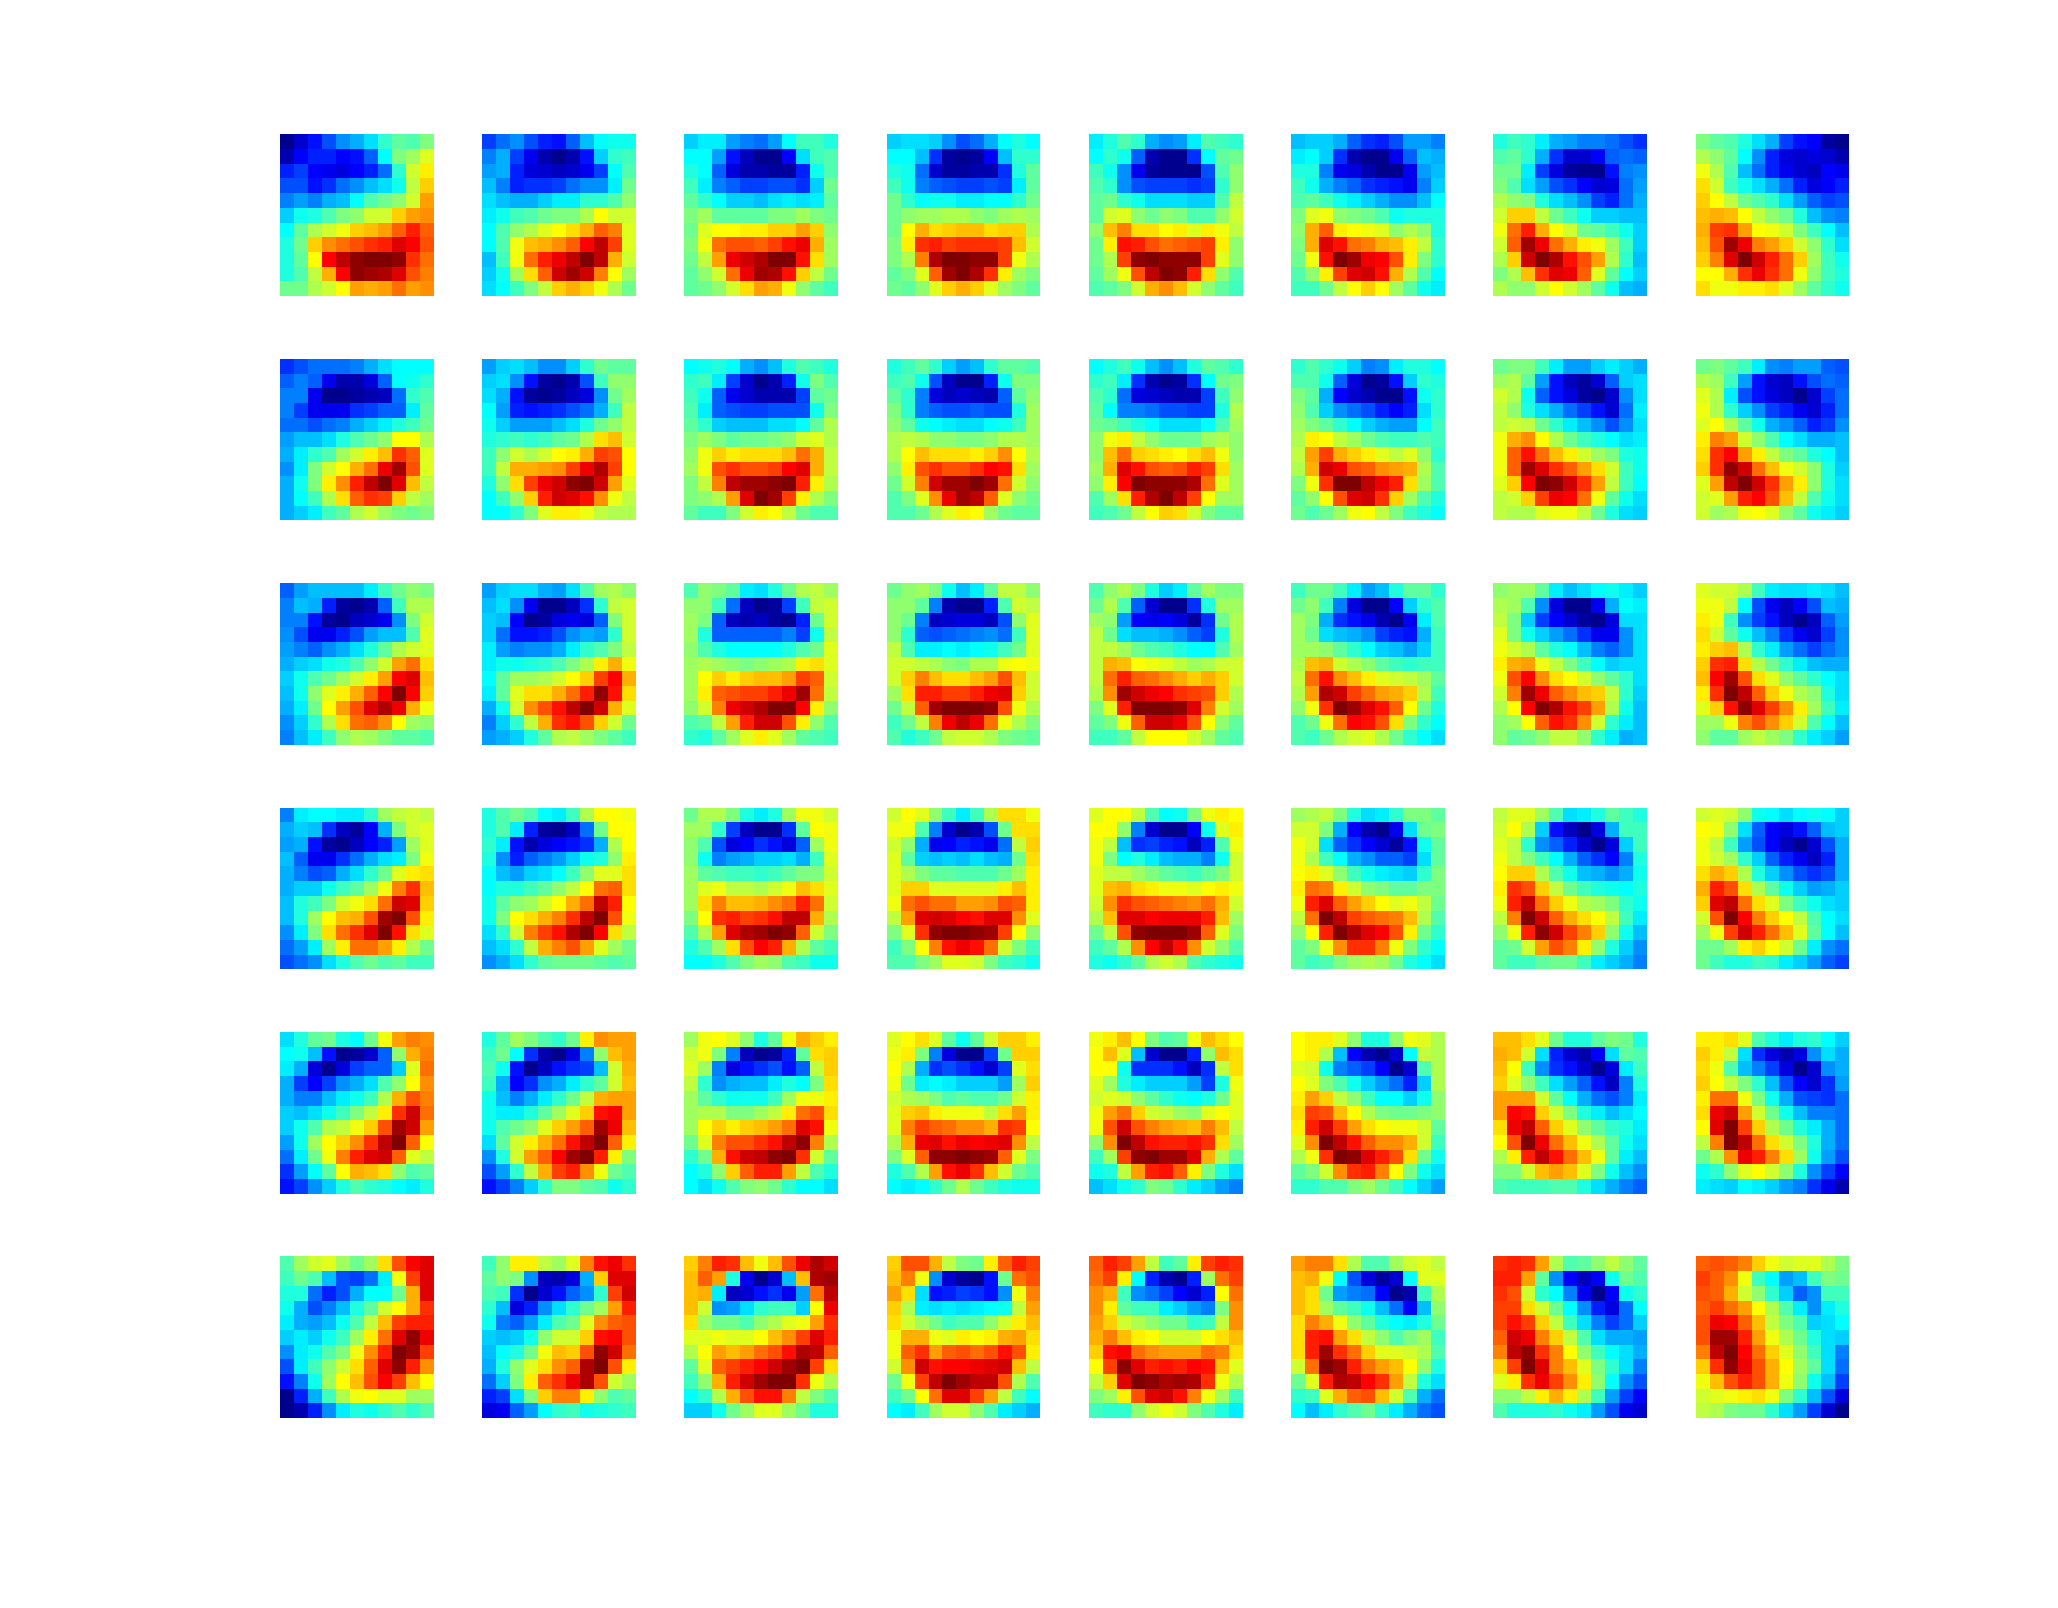
\includegraphics[width=\textwidth]{mean_scallop_quadrants}
      \caption{}
      \label{subfig:mean_quadrant}
  \end{subfigure}
  \begin{subfigure}[]{0.45\textwidth}
      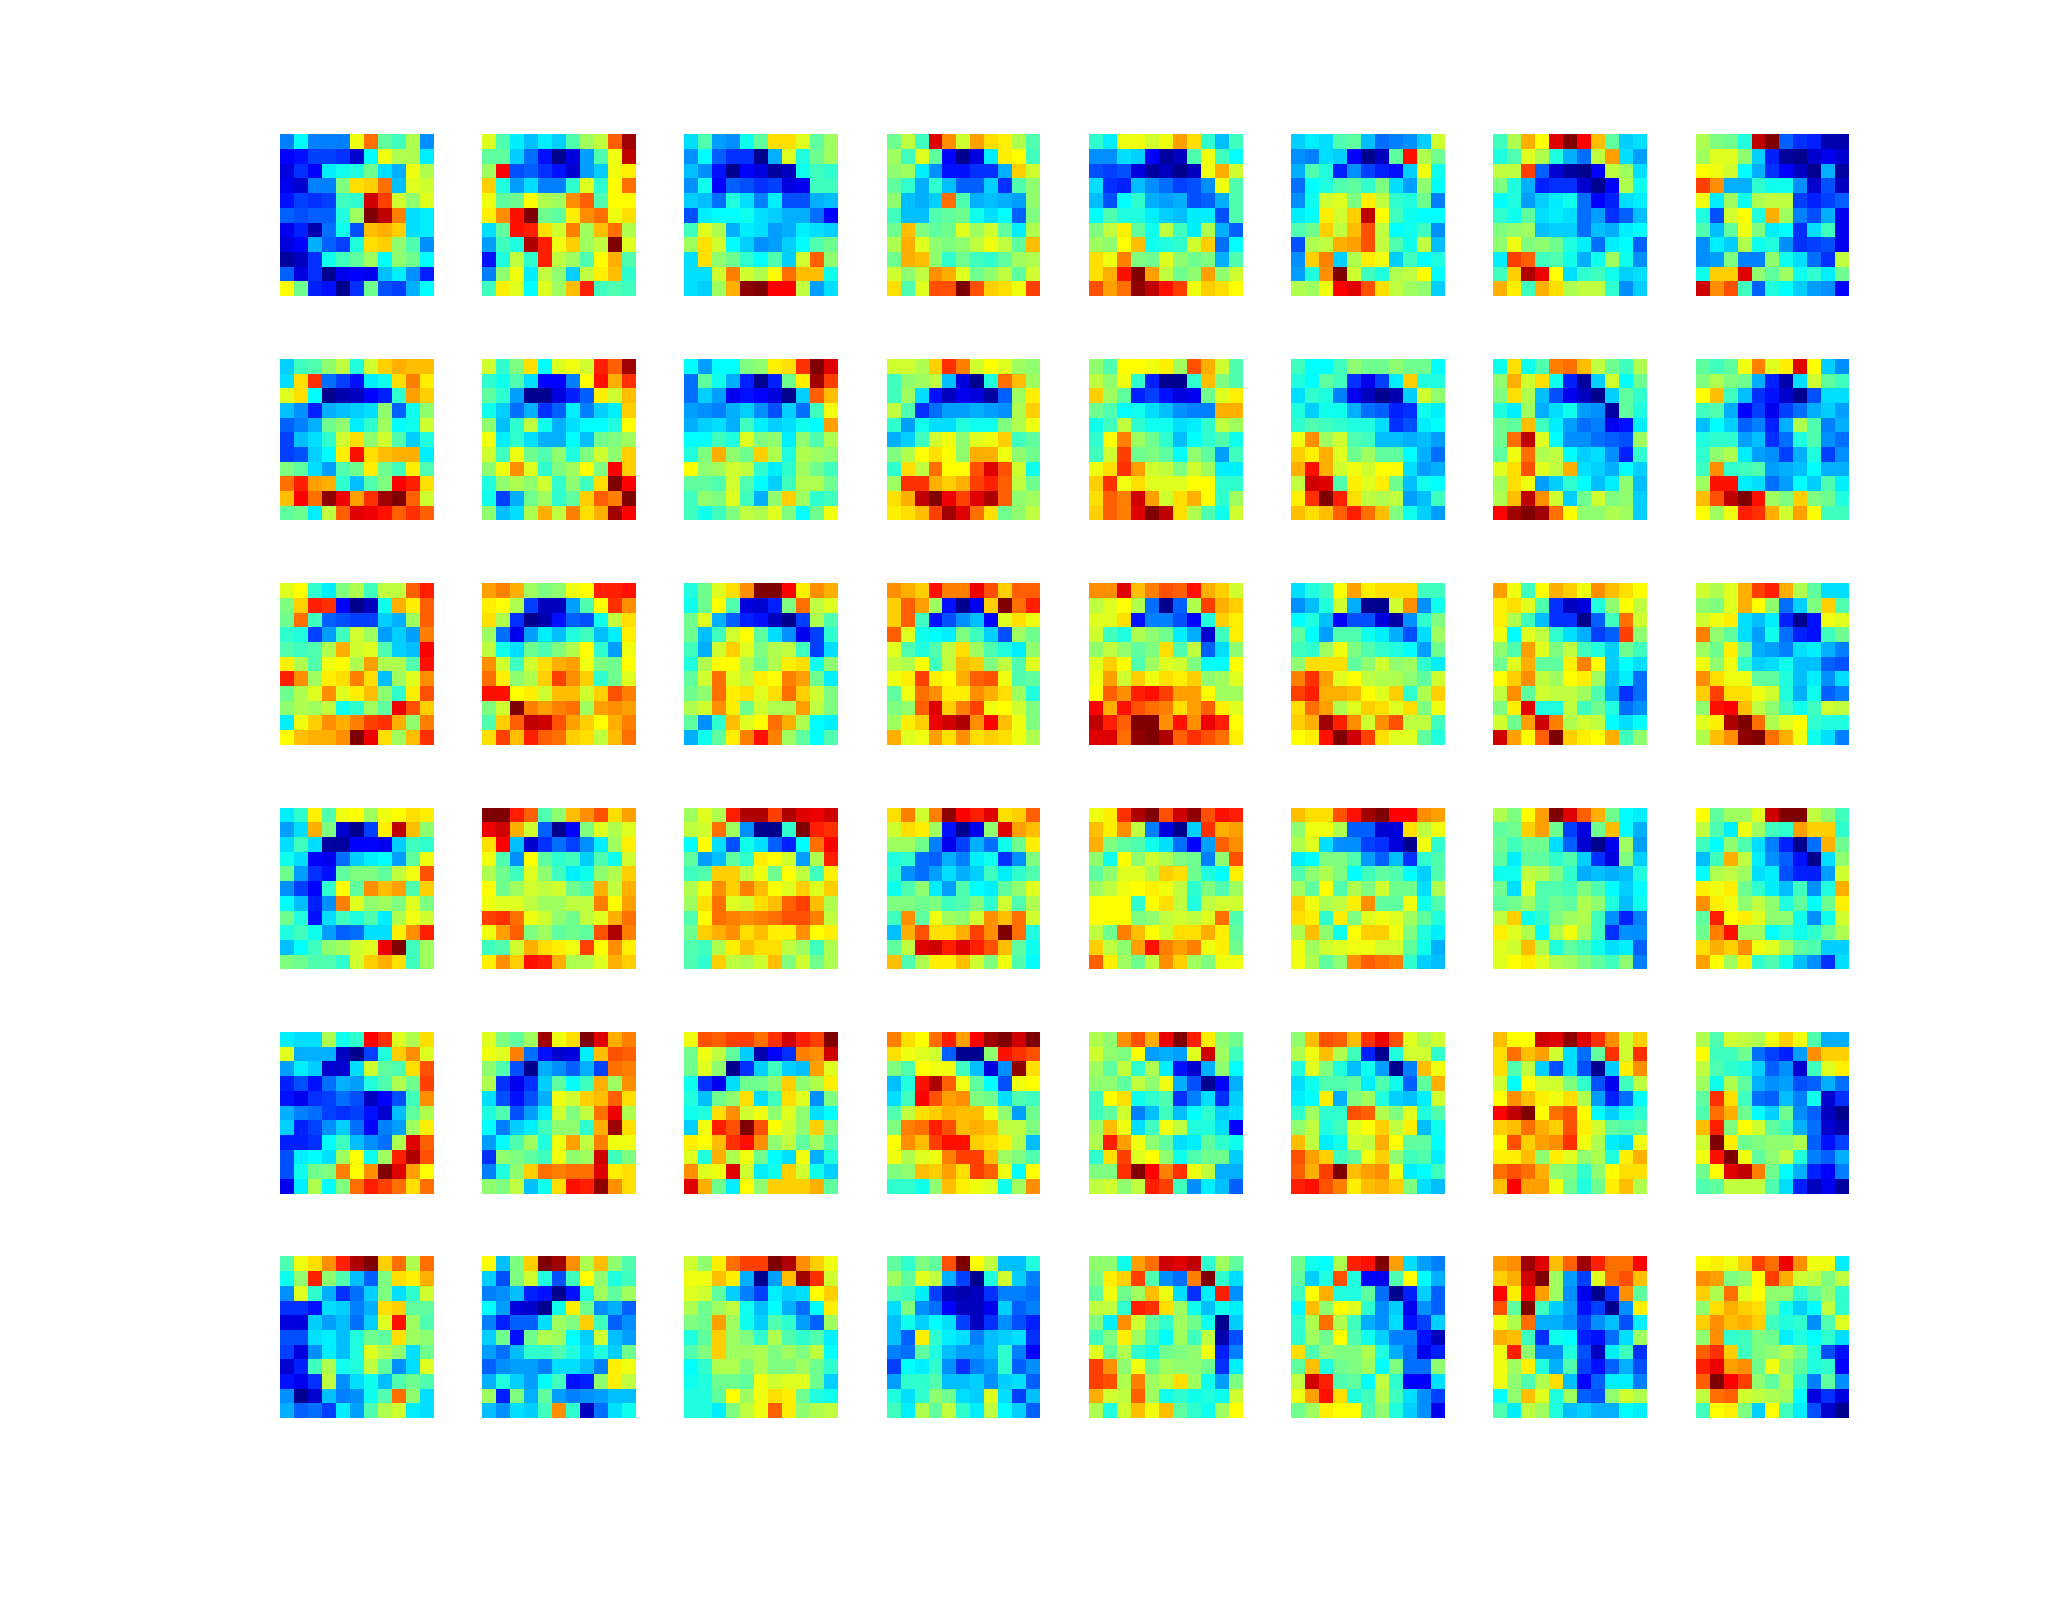
\includegraphics[width=\textwidth]{stddev_scallop_quadrants}        
      \caption{}
      \label{subfig:stddev_quadrant}
  \end{subfigure}
  \caption[Mean and variance map of scallops in each quadrant]{(\subref{subfig:mean_quadrant}) Mean map of scallops in each quadrant; (\subref{subfig:stddev_quadrant}) Standard deviation map of scallops in each quadrant.
  Red corresponds to higher numeric values and blue correspond to lower numeric values.}
  \label{fig:mean_stddev_quadrant}
\end{figure*}



\subsubsection{Scallop Profile Learning} \label{subsubsec:scallop_profile_learning}

The statistics of the dataset of $3\,706$ images, used to build the illustration in Figure~\ref{fig:mean_stddev_quadrant}, form a look-up table that represents reference scallop profile (mean and standard deviation maps) 
as a function of scallop center pixel location.
To obtain the reference profile for a pixel location, 
the statistics from all the scallops whose centers lie inside a $40\times40$ window centered on the pixel is used.
This look-up table can be compressed; it turns out that not all of the 121 bins ($11\times11$) within each map is equally informative, because bins close to the boundary are more likely to include a significant number of background pixels.
For this reason, a circular mask with a radius covering 4 bins is applied to each map (Figure~\ref{fig:scallop_learning_mask}), thus reducing the number of bins that are candidates as features for identification to $61$.
Out of these $61$ bins, $15$ additional bins having the highest standard deviation are ignored, leading to a final set of $46$ bins.
The value in the selected $46$ bins from mean map forms a $46$-dimensional feature vector associated with that region. The corresponding $46$ bins from the standard deviation map are also recorded, and are used to weight the features
(as seen later in \eqref{distance}).

\begin{figure}
  \centering
  \begin{subfigure}[]{0.3\textwidth}
      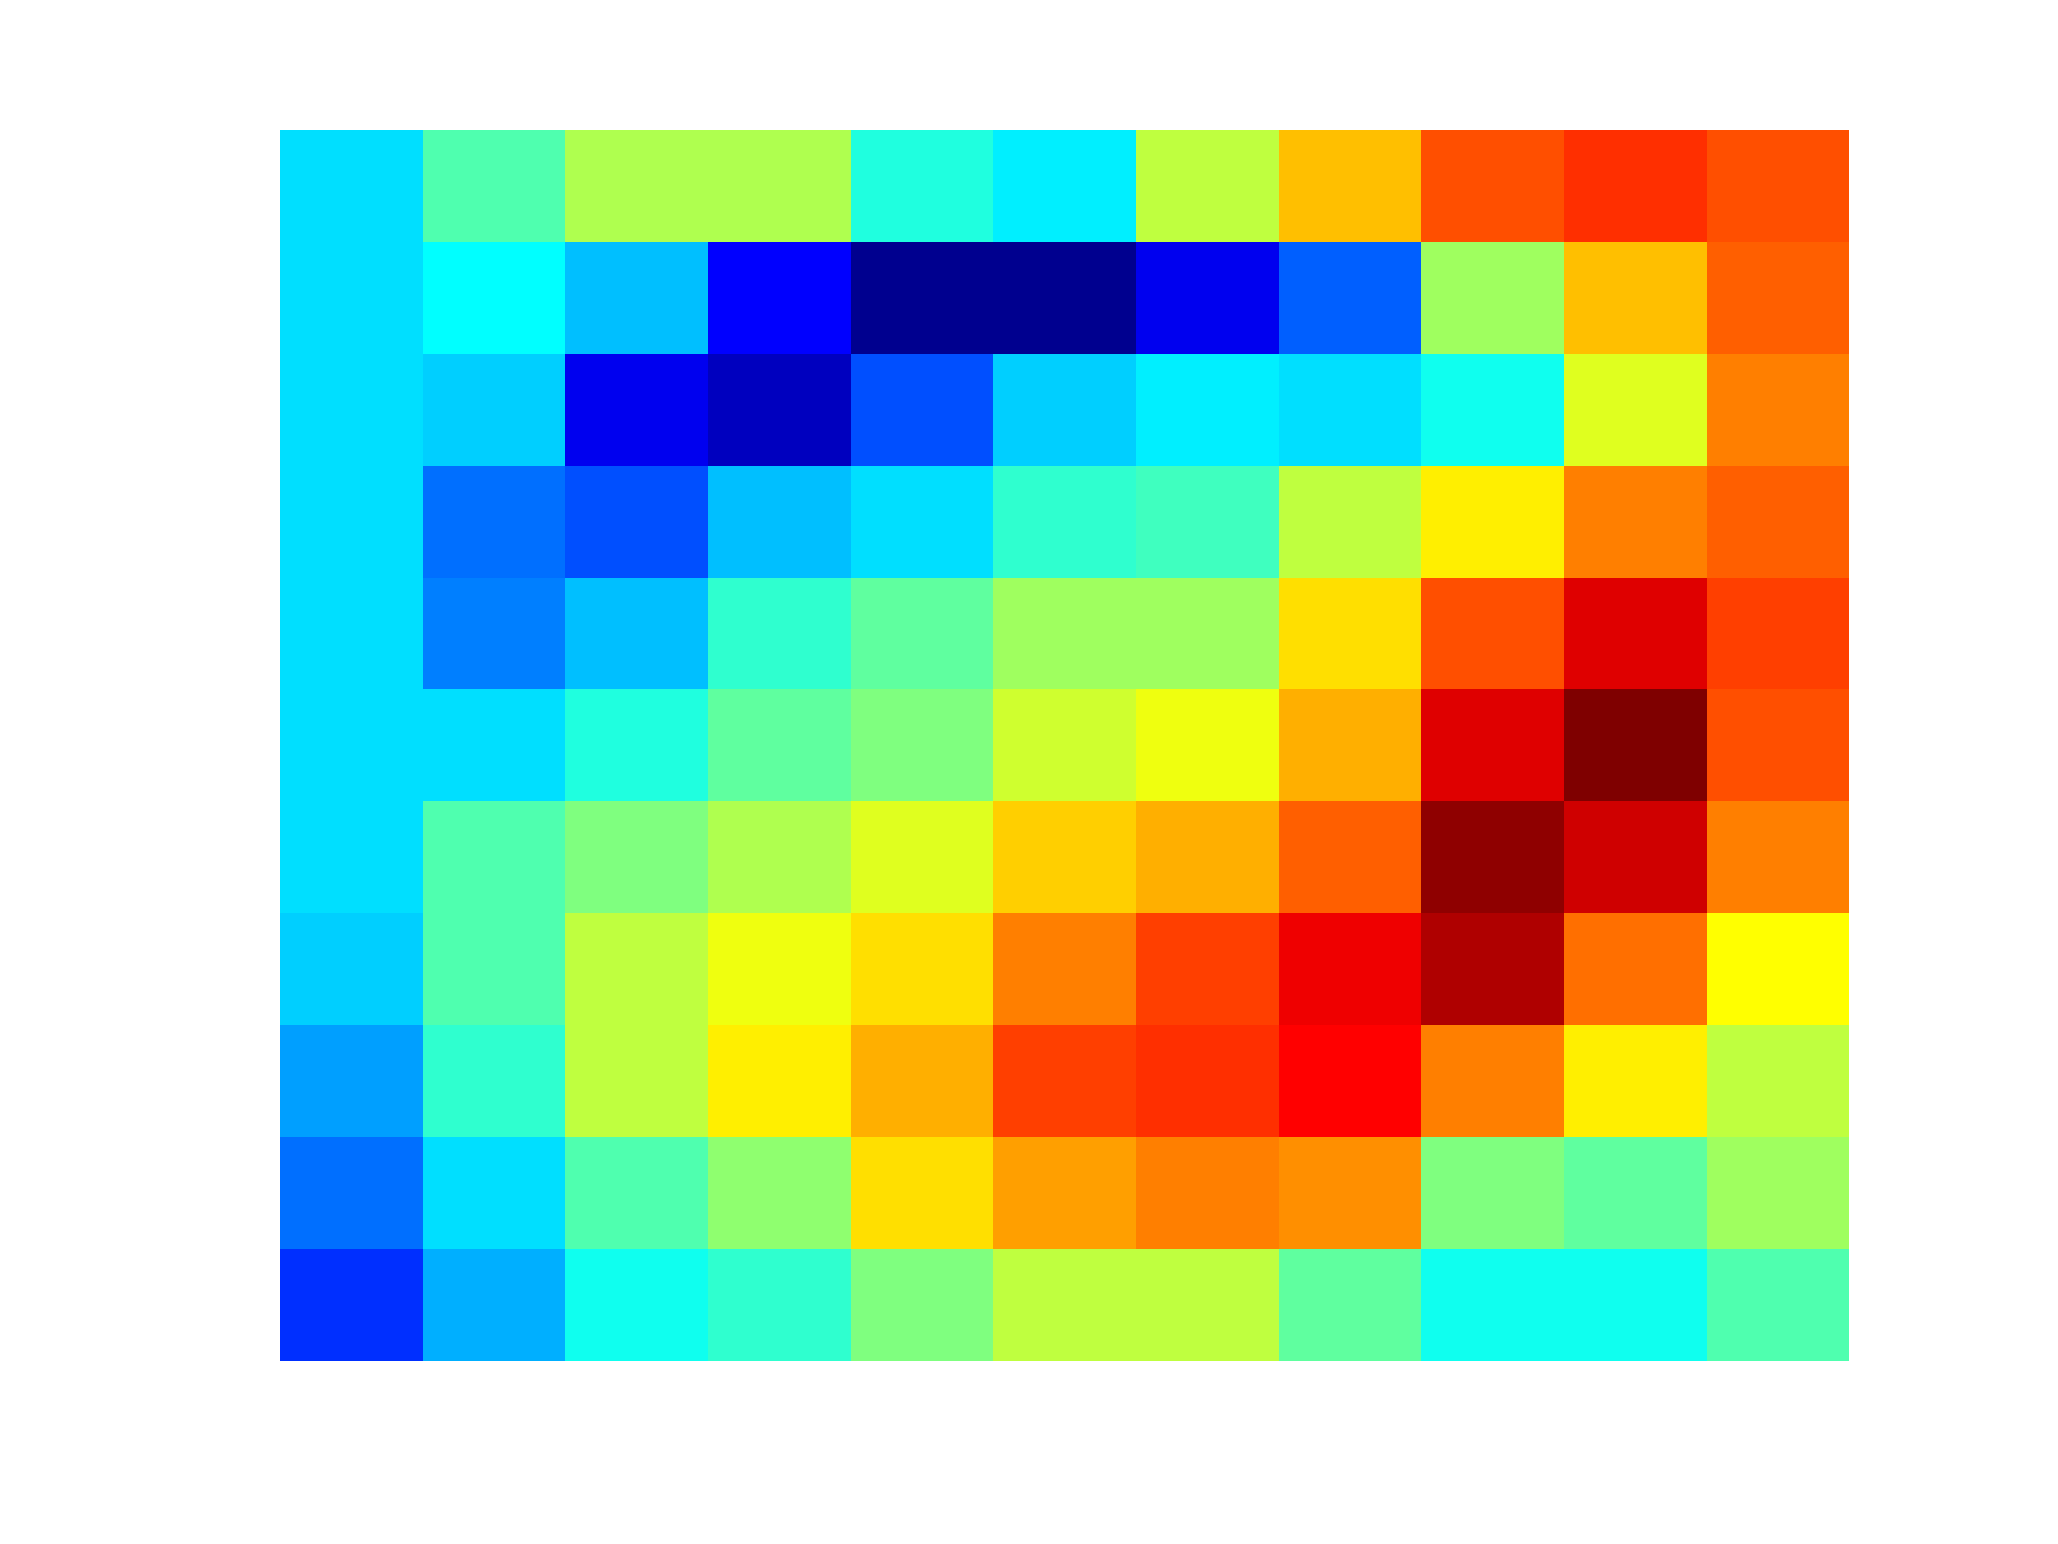
\includegraphics[width=\textwidth]{curr_scallop_mean}
      \caption{}
      \label{subfig:mean_scallop}
  \end{subfigure}
  \begin{subfigure}[]{0.3\textwidth}
      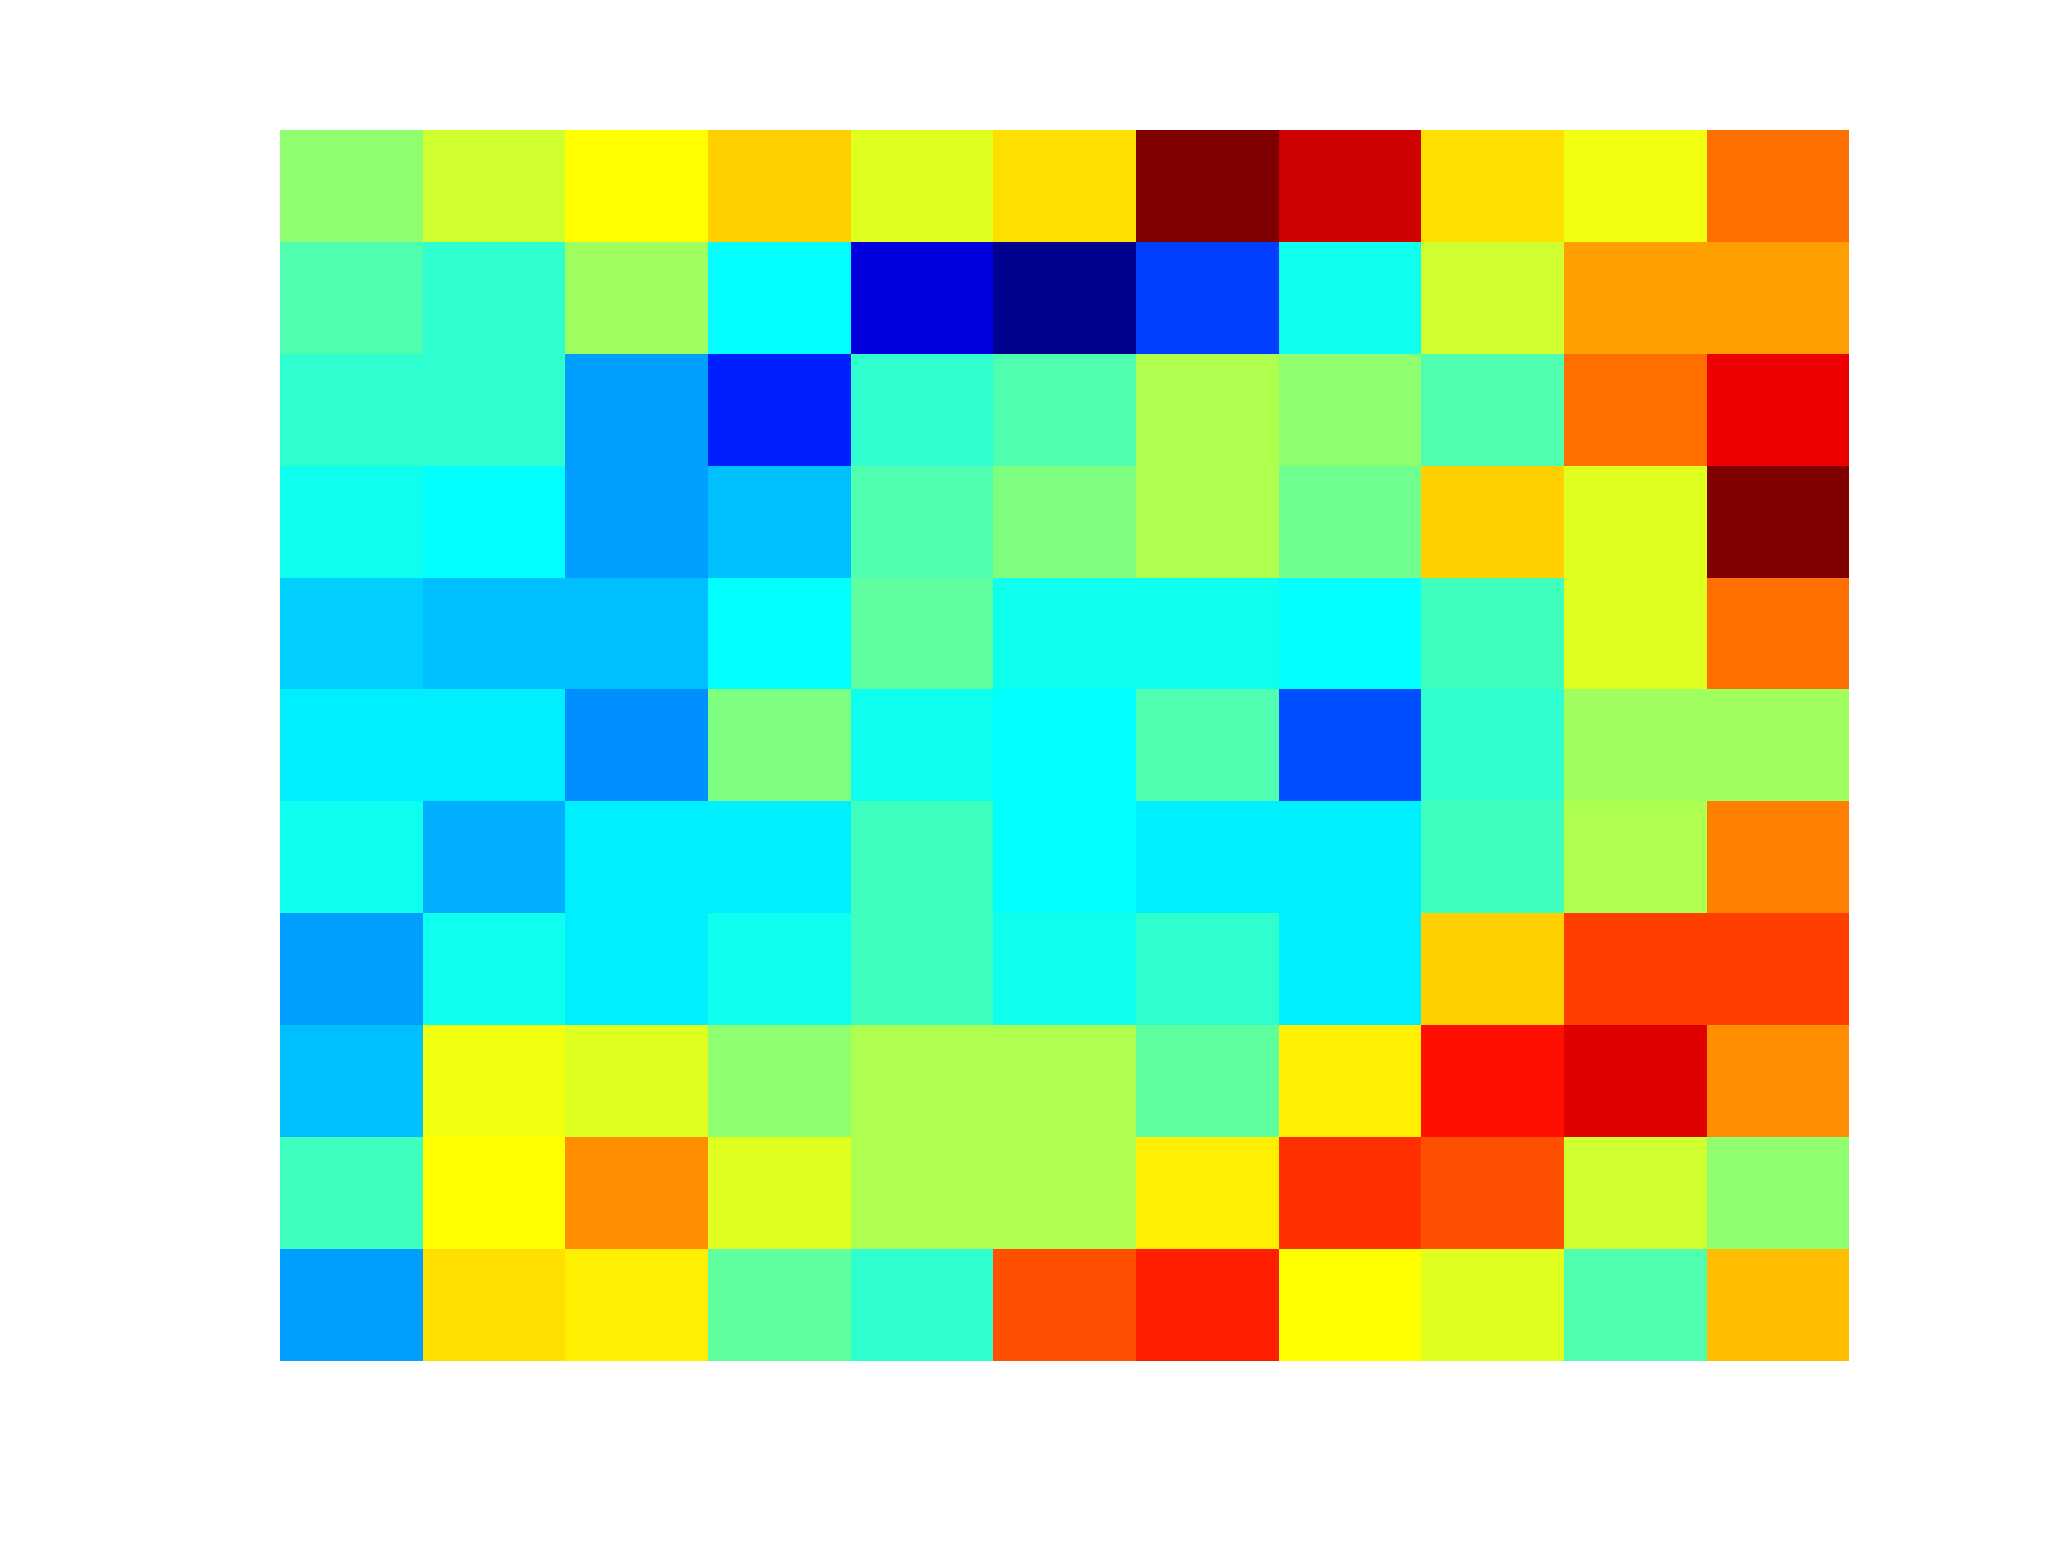
\includegraphics[width=\textwidth]{curr_scallop_stddev}
      \caption{}
      \label{subfig:stddev_scallop}
  \end{subfigure}
  \begin{subfigure}[]{0.3\textwidth}
      
\includegraphics[width=\textwidth]{mask_centered}
      \caption{}
      \label{subfig:mask_scallop}
  \end{subfigure}
  \caption[Illustration of scallop profile hypothesis]{Intensity statistics and mask for a region centered at image coordinates $(470,63)$: (\subref{subfig:mean_scallop}) Map of mean intensity; (\subref{subfig:stddev_scallop}) Map of intensity standard deviation;
  (\subref{subfig:mask_scallop}) Mask applied to remove background points.}
  \label{fig:scallop_learning_mask}
\end{figure}


\subsubsection{Scallop Template Matching} \label{subsubsec:scallop_template_matching}

With this look-up table that codes the reference scallop profile for every scallop center pixel location,
the resemblance of any segmented object to a scallop can now be assessed.
The metric used for this comparison is a weighted distance function between the 
elements of the feature vector for the region corresponding to the segmented object, and that coming from the look-up table, depending on the location of the object in the image being processed.
If this distance metric is below a certain threshold $D_\mathsf{thresh}$, the object is classified
a scallop.
Technically, let $X^o=(X^o_1,X^o_2, \ldots,X^o_{46})$ denote the feature vector computed for the segmented object,
and $X^s=(X^s_1,\ldots,X^s_{46})$ the reference
feature vector. 
Every component of the $X^s$ vector is a reference mean intensity value for a particular bin, and is associated with a standard deviation $\sigma_k$ from the reference standard deviation map.
%(Section~\ref{subsubsec:scallop_profile_hypothesis}).
To compute the distance metric, first normalize $X^o$ to produce vector $X^{\bar{o}}$ with components 
%
\[
X^{\bar{o}}_p = \min_{k} X^s_k + \left(\frac{\max \limits_{k} X^s_k-\min \limits_{k} X^s_k}{\max \limits_{k} X^o_k-\min \limits _{k} X^o_k}
\right)\left[ X^o_p-\min_{k} X^o_k \right] \;\text{for } p=1,\ldots,46\enspace,
\]
%
and then evaluate the distance metric $D_{t}$ quantifying the dissimilarity between the normalized object vector $X^{\bar{o}}$ and the reference feature vector $X^s$ as
%
\begin{equation}\label{distance}
D_{t} = \sqrt{\sum_{k=1}^n\frac{\|X^{\bar{o}}_{k}-X^s_k\|^2}{\sigma_k}} \enspace .
\end{equation}
%

%
\begin{figure}
\centering
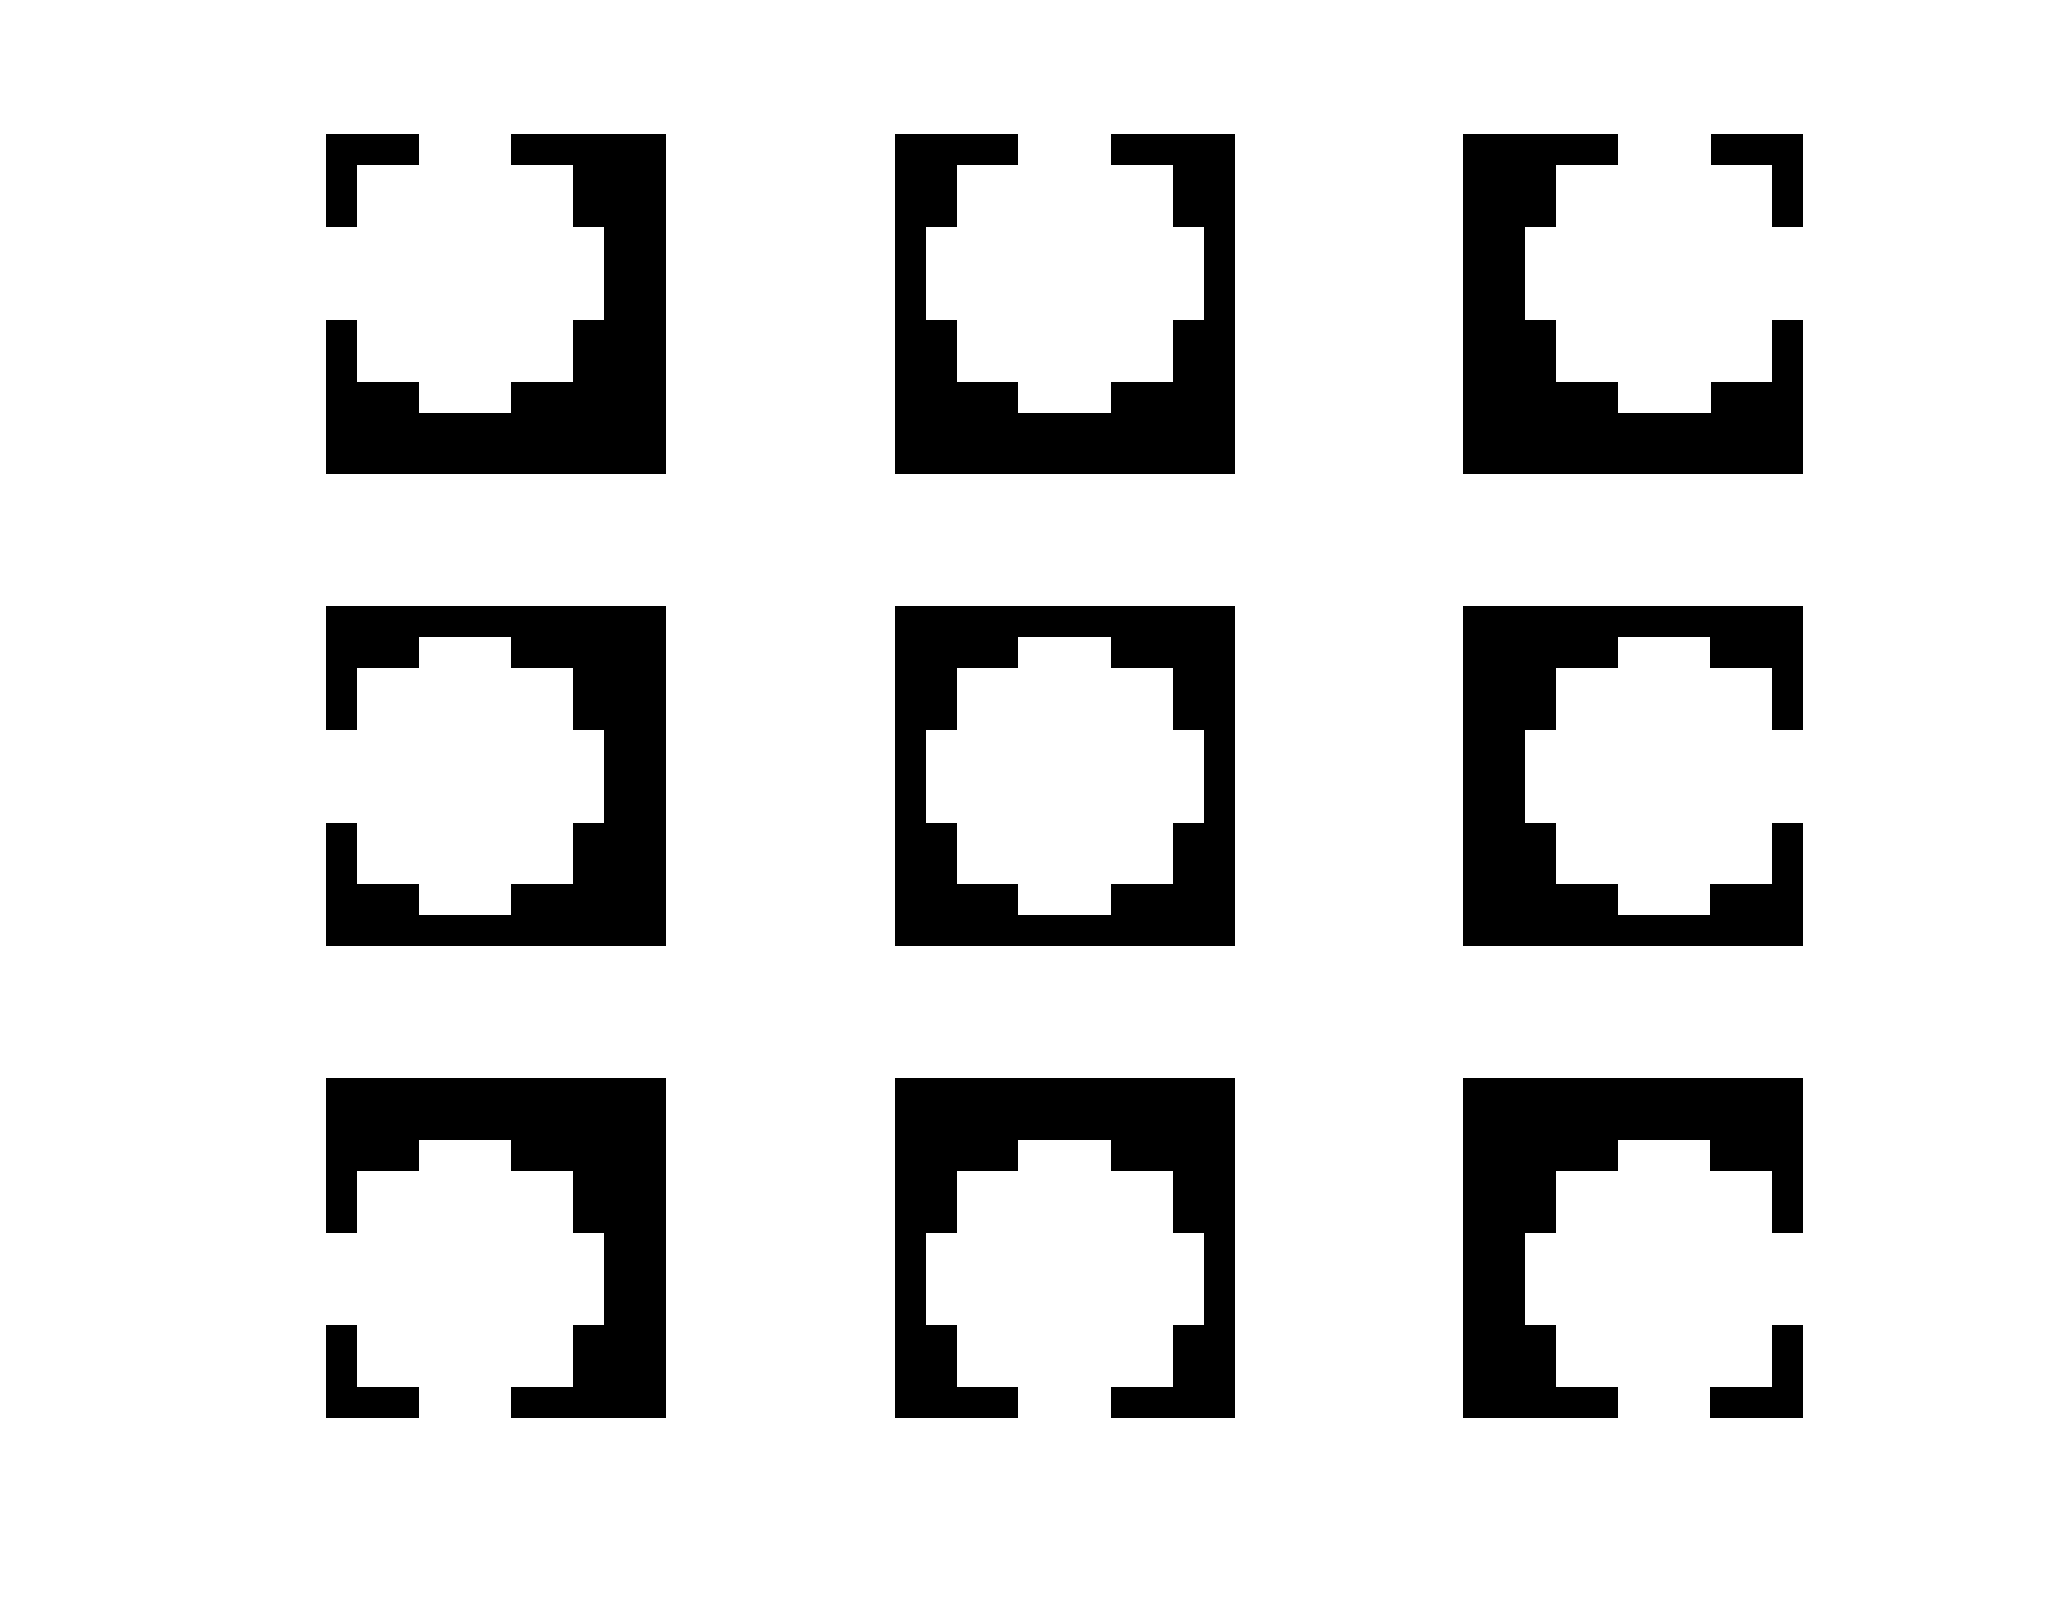
\includegraphics[width=0.6\textwidth]{mask_offset}
\caption[Template matching masks]{Nine different masks slightly offset from the center used to make the classification layer
robust to errors in segmentation}
\label{fig:scallop_masks}
\end{figure}
%

Small variations in segmentation can produce notable deviations in the computed distance metric \eqref{distance}.
To alleviate this effect, the mask of Figure~\ref{subfig:mask_scallop} was slightly shifted in different directions and the best match in terms of the distance was identified.
This process enhanced the robustness of the classification layer with respect to  small segmentation errors.
Specifically, nine slightly shifted masks were used (shown in
Figure~\ref{fig:scallop_masks}).  Out of the nine resulting
distance metrics $D^{o_1}_t$ \ldots $D^{o_9}_t$, the smallest $
 D_\mathsf{obj}=\min_{p\in\{1,\ldots,9\}} D^{o_p}_t
$ is found and used for classification. 
If $D_\mathsf{obj}<D_\mathsf{thresh}$, 
the corresponding object
is classified as a scallop.
Based on Figures~\ref{subfig:precision_recall}--\ref{subfig:template_hist},
the threshold value was chosen at $D_\mathsf{thresh}=7$ to give a recall\footnote{\emph{Recall} refers to the fraction of relevant instances
identified: fraction of scallops detected over all ground truth scallops;
\emph{precision} is the fraction of the instances returned that are really relevant
compared to all instances returned: fraction of true scallops over all objects
identified as scallops.} rate of 
$97\%$.
Evident in Figure~\ref{subfig:precision_recall} is the natural trade-off between increasing recall rates and keeping the number of false positives low.

%
\begin{figure*}
  \centering
  \begin{subfigure}{0.47\textwidth}
      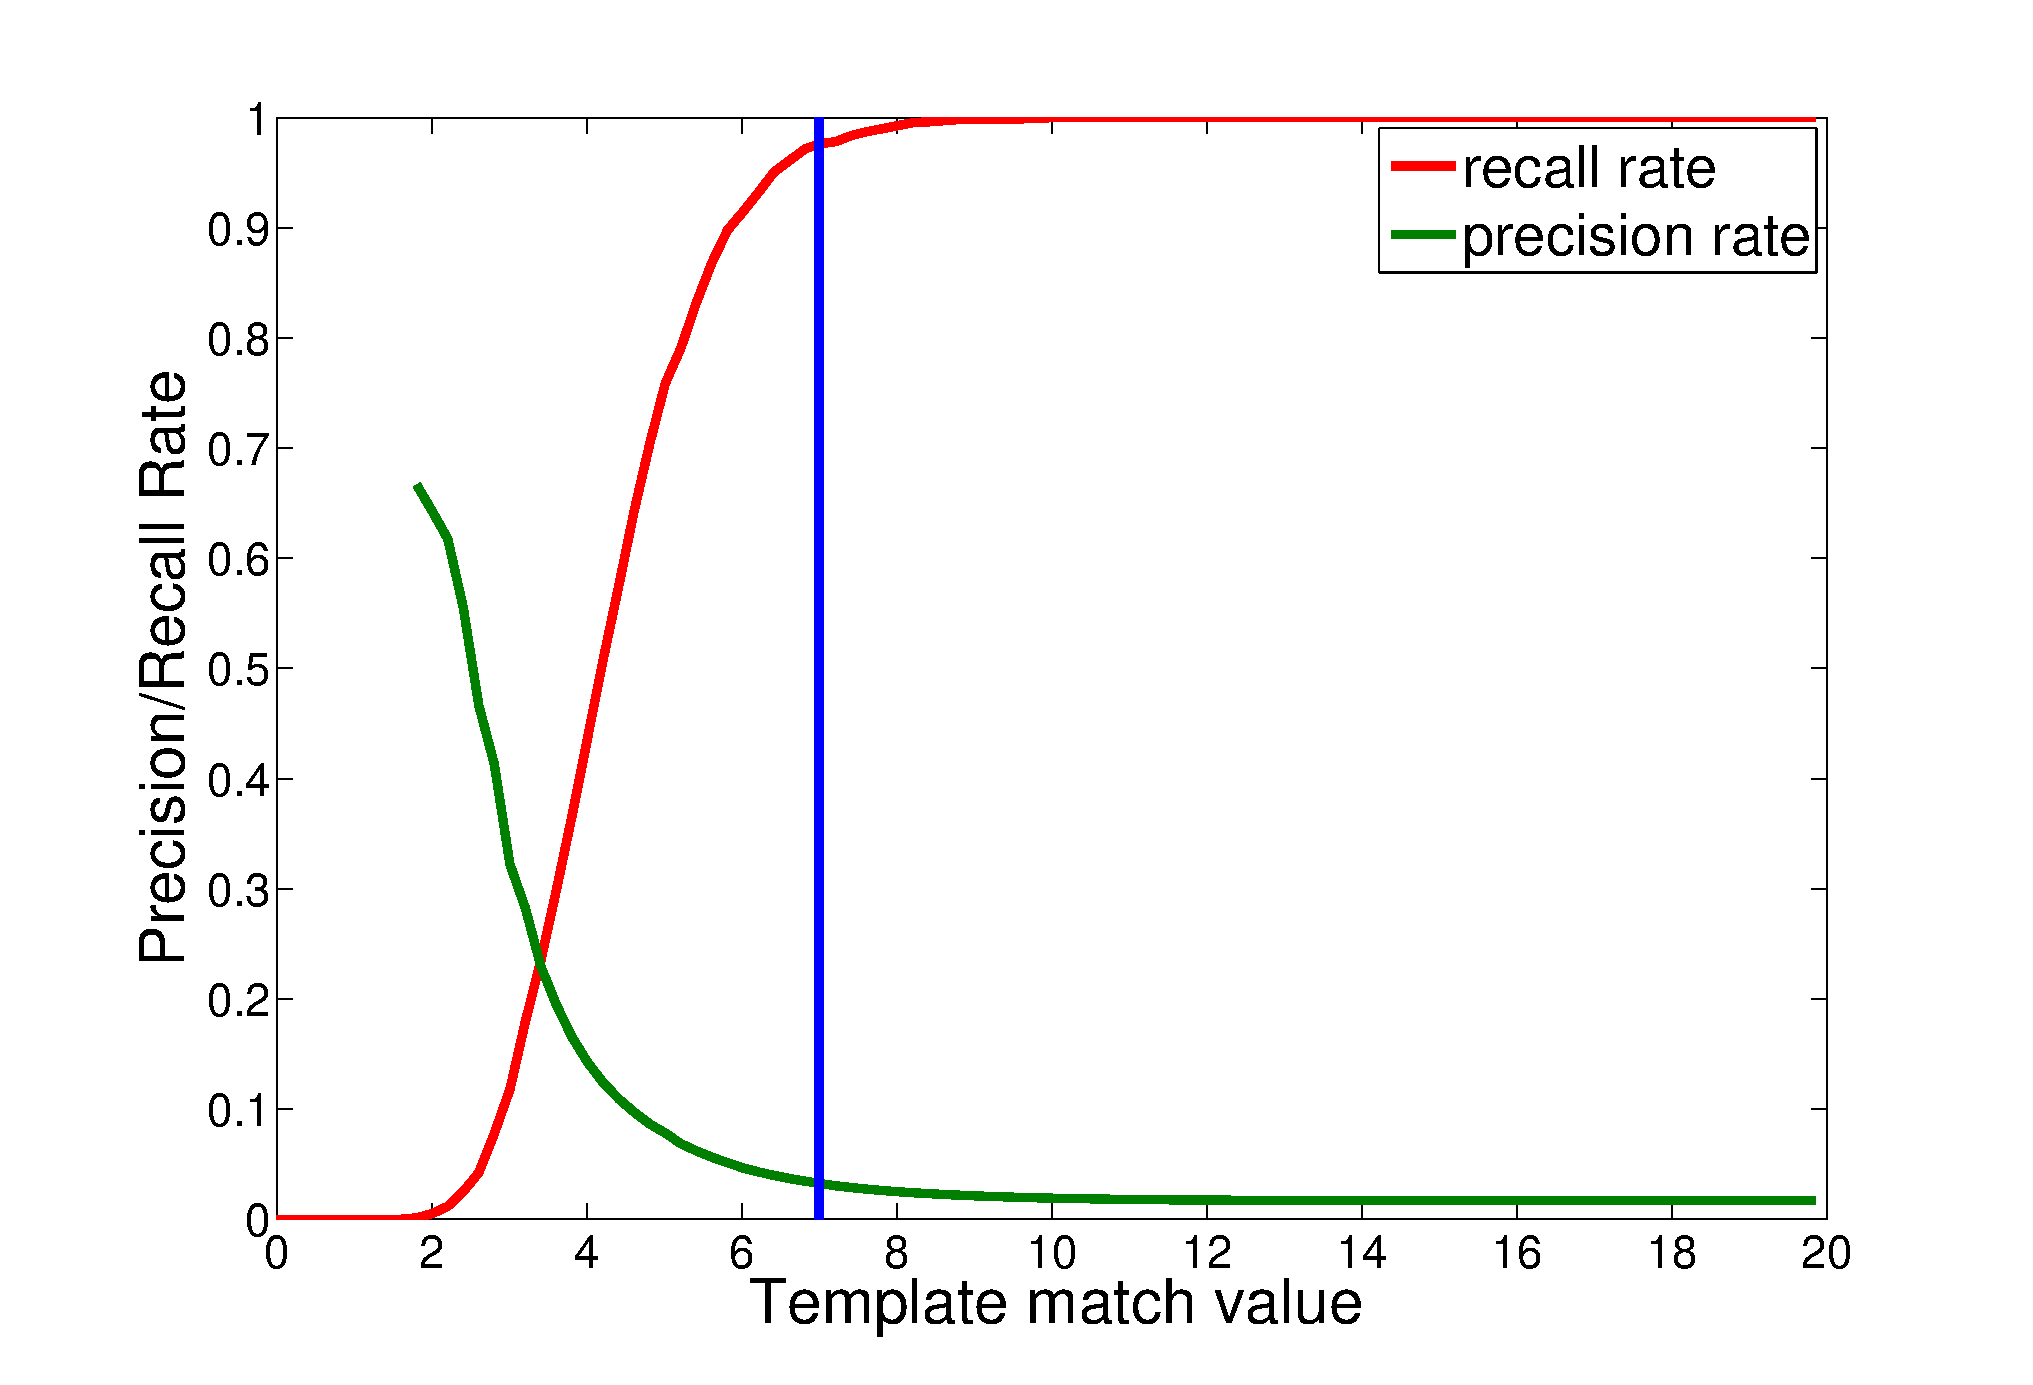
\includegraphics[width=\textwidth]{precision_recall}
      \caption{}
      \label{subfig:precision_recall}
  \end{subfigure}
  \begin{subfigure}{0.47\textwidth}
      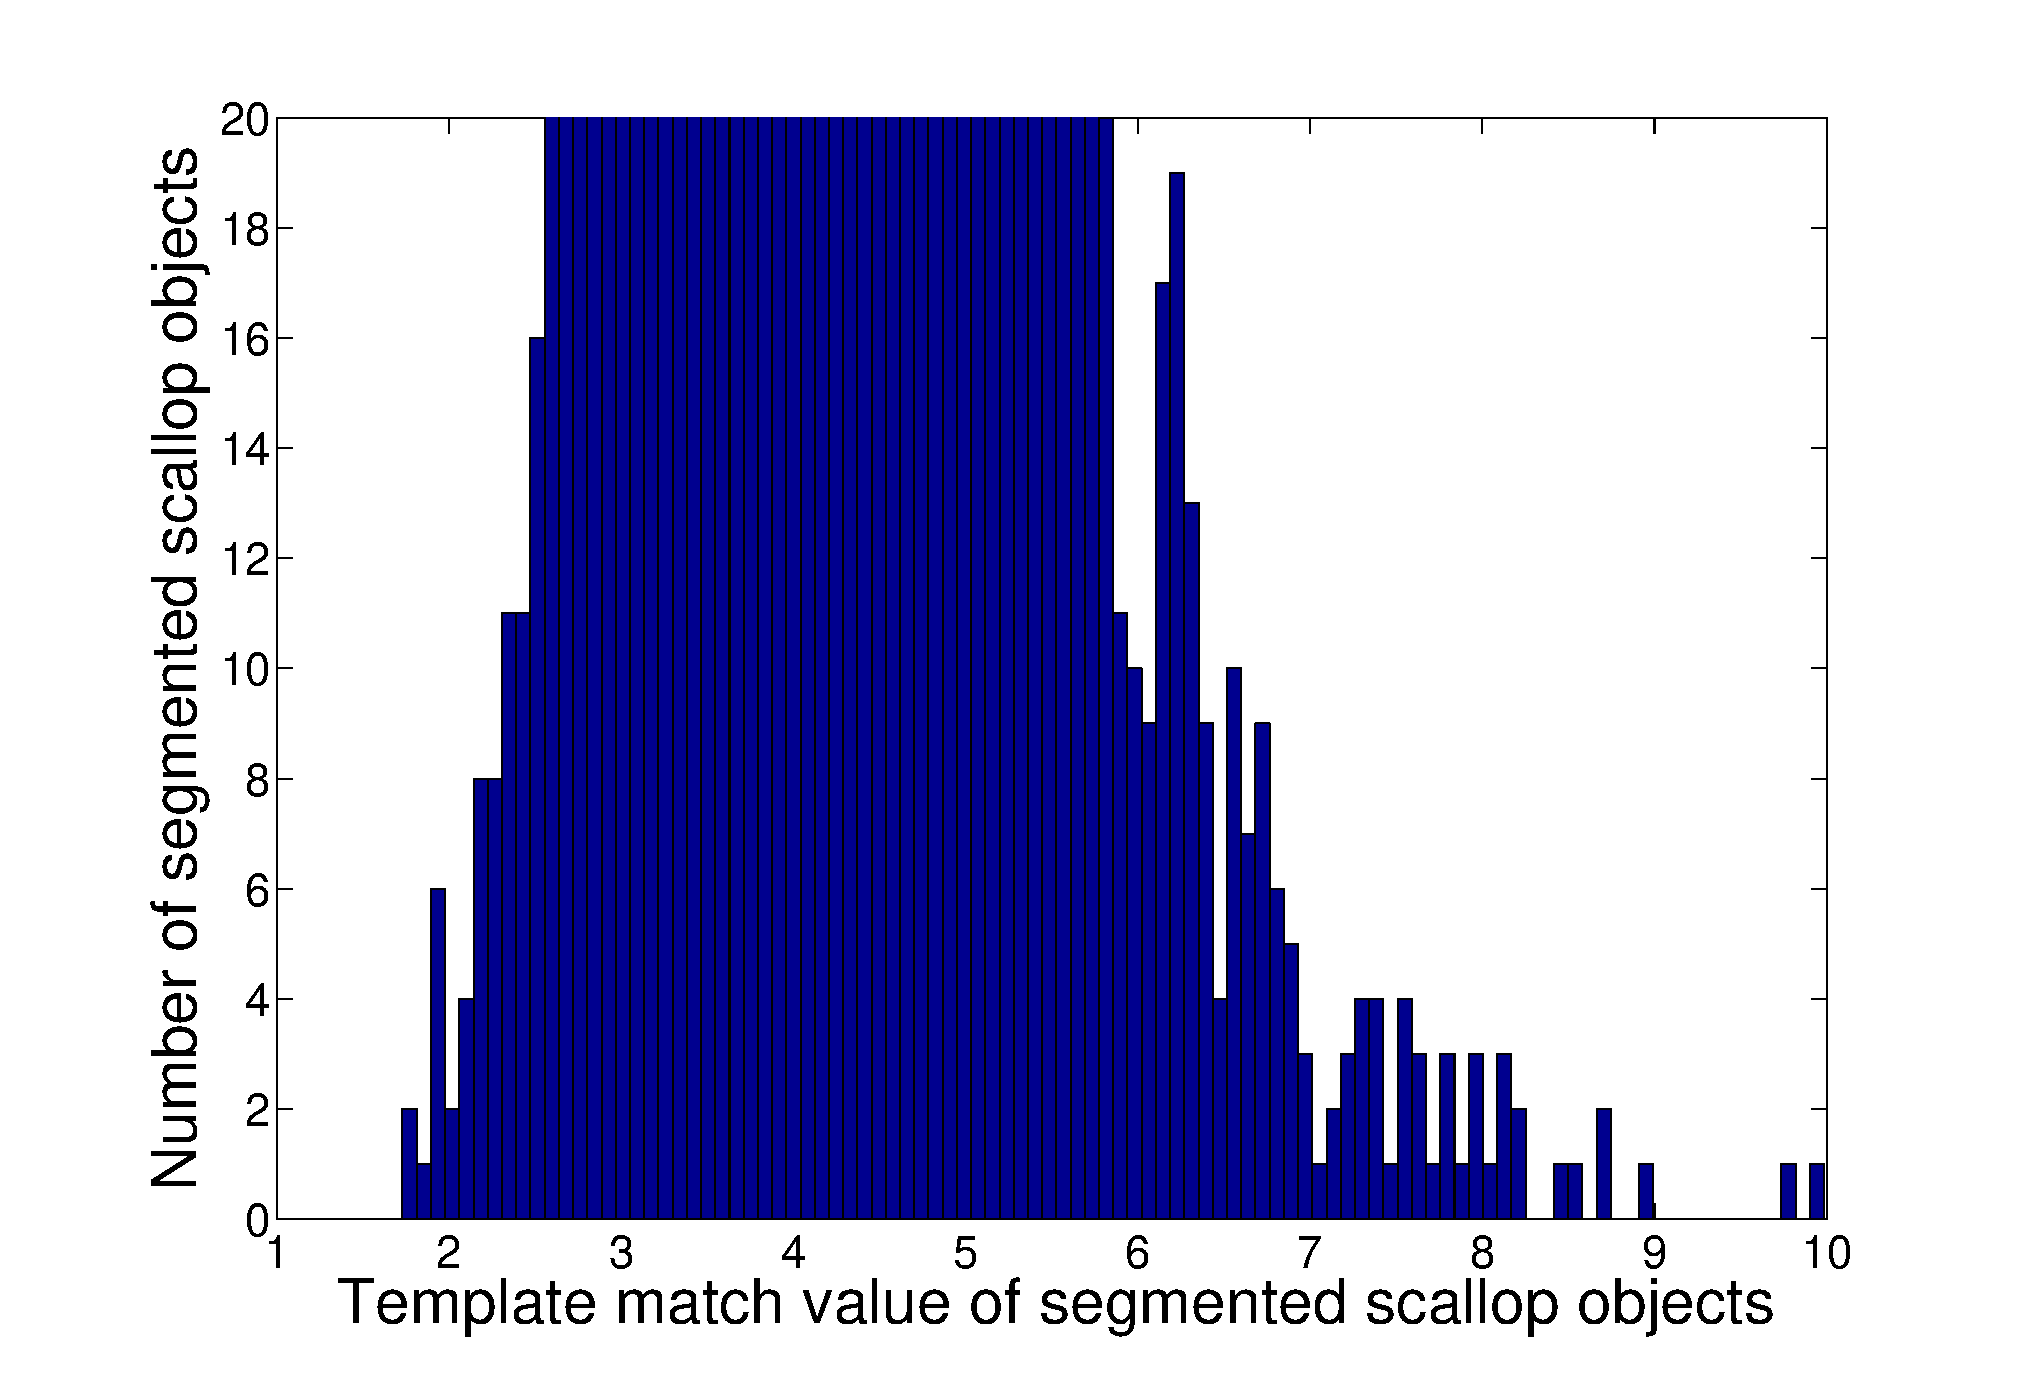
\includegraphics[width=\textwidth]{template_thresh_hist}         
      \caption{}
      \label{subfig:template_hist}
  \end{subfigure}
  \caption[Precision-Recall curves for Classification Layer]{(\subref{subfig:precision_recall}) Precision-Recall curve with $D_\mathsf{thresh}$ shown as
  a vertical line; (\subref{subfig:template_hist}) 
  Histogram of template match of segmented scallop objects.}
  \label{detection-curves}
\end{figure*}
%========================================================================================
\subsection{Layer IV: False Positives Filter}

To decrease the false positives that are produced in the classification layer, two methods are evaluated as possible candidates: a high-dimensional \gls{wctm} technique and a \gls{hog} method. 
The main objective here is to find a method that will retain a high percentage of true positive scallop and at the same time eliminate as many false positives from the classification layer as possible.

\subsubsection{High-dimensional weighted correlation template matching (WCTM)}
In this method, the templates used are generated from scallop images that are \emph{not} preprocessed, i.e., images that are not median-filtered, unlike the images that were processed by the first three layers. 
The intuition behind this is that although median filtering reduces speckle noise and may improve the performance of segmentation, it also weakens the edges and gradients in an image. 
Avoiding median filtering helps to generate templates that are more accurate than the ones already used in the classification layer.

Based on the observation that the scallop templates are dependent on their position in the image (Figure~\ref{fig:mean_stddev_quadrant}), a new scallop template is generated for each object that is classified as a scallop in Layer III. 
As indicated earlier, such an object would be represented by a triplet $(a_o,b_o,R_o)$, where $a_o$ and $b_o$ represent the spatial Cartesian coordinates of object's geometric center, and $R_o$ gives its radius. 
The representative scallop template is now generated from all scallops in the learning set (containing 3\,706 scallops), of which the center is within a $40\times40$ window in the neighborhood of the object center $(a_o,b_o)$. 
Each of these scallops is then extracted using a window of size $2.5R\times2.5R$ where $R$ is the scallop radius. 
Since these scallops in the learning set can be of different dimensions, it is resized (scaled) to a window of size $2.5R_o\times2.5R_o$. 
All these scallop instances in the learning set are finally combined through a pixel-wise mean to obtain the mean representative template. 
Similarly, a standard deviation map that captures the standard deviation of each pixel in the mean template is also obtained.  
The templates produced here are of larger size compared to the templates in Layer III (recall that a Layer III template was of size $11\times11$).
The inclusion of slightly more information contributes to these new larger templates being more accurate.

In a fashion similar to the analysis in Layer III, the templates and object pixels first undergo normalization and mean subtraction.
Then they are compared.
Let $v=(2.5R_o)^2$ be the total number of pixels in both the template and the object, and let the new reference scallop feature (template) and the object be represented by vectors $X^t=(X^t_1,X^t_2, \ldots,X^t_{v})$ and $X^u=(X^u_1,\ldots,X^u_{v})$, respectively. 
In addition, let $\sigma$ be the standard deviation vector associated with $X^t$.
Then the reference scallop feature vector $X^t$ would first be normalized as follows: 
%
\[
X^{t'}_p = \min_{k} X^u_k + \left(\frac{\max \limits_{k} X^u_k-\min \limits_{k} X^u_k}{\max \limits_{k} X^{t}_k-\min \limits _{k} X^{t}_k}
\right)\left[ X^{t}_p-\min_{k} X^{t}_k \right] \; ,
\]
%
where $p$ denotes the position of component $X^t_p$ in vector $X^t$.
Normalization is followed by mean subtraction, this time both for the template and for the object. 
The resulting, mean-subtracted reference scallop feature $X^{\bar{t}}$, and object $X^{\bar{u}}$ are computed as
%
\begin{align*}
X^{\bar{t}}_p &= X^{t'}_p-\frac{1}{v}\sum_{k=1}^{v}X^{t'}_k \enspace,& 
X^{\bar{u}}_p &= X^{u}_p-\frac{1}{v}\sum_{k=1}^{v}X^{u}_k \enspace.
\end{align*}
%
Now the standard deviation vector is normalized:
%
\[
\bar{\sigma}_p = \frac{\sigma_p}{\sum_{k=1}^{v}\sigma_k} \enspace.
\]
%
At this point, a metric that expresses the correlation between the mean-subtracted template and the object can be computed.
This metric is weighted by the (normalized) variance of each feature. 
In general, the higher the value of this metric, the better the match between the object and the template. 
The \gls{wctm} similarity metric is given by
%
\[
D_\mathsf{wctm} = \sum_{k=1}^v\frac{X^{\bar{t}}_{k}X^{\bar{u}}_k}{\bar{\sigma}_{k}} \enspace .
\]
%
The threshold set for the weighted correlation metric $D_\mathsf{wctm}$, in order to distinguish between likely true and false positives is at $0.0002222$, i.e., any object with a similarity score lower than this threshold is rejected. 
This threshold value is justified from the precision-recall curves (see Figure~\ref{subfig:layer4_precision_recall}) of the weighted correlation metric values for the objects filtering down from the classification layer. 
The threshold shown by the blue line corresponds to 96\% recall rate, i.e., 96\% of the true positive scallops from the classification layer pass through \gls{wctm}. 
At the same time, \gls{wctm} decreases the false positives by over 63\%.
%
\begin{figure}
  \centering
  \begin{subfigure}{0.45\textwidth}
      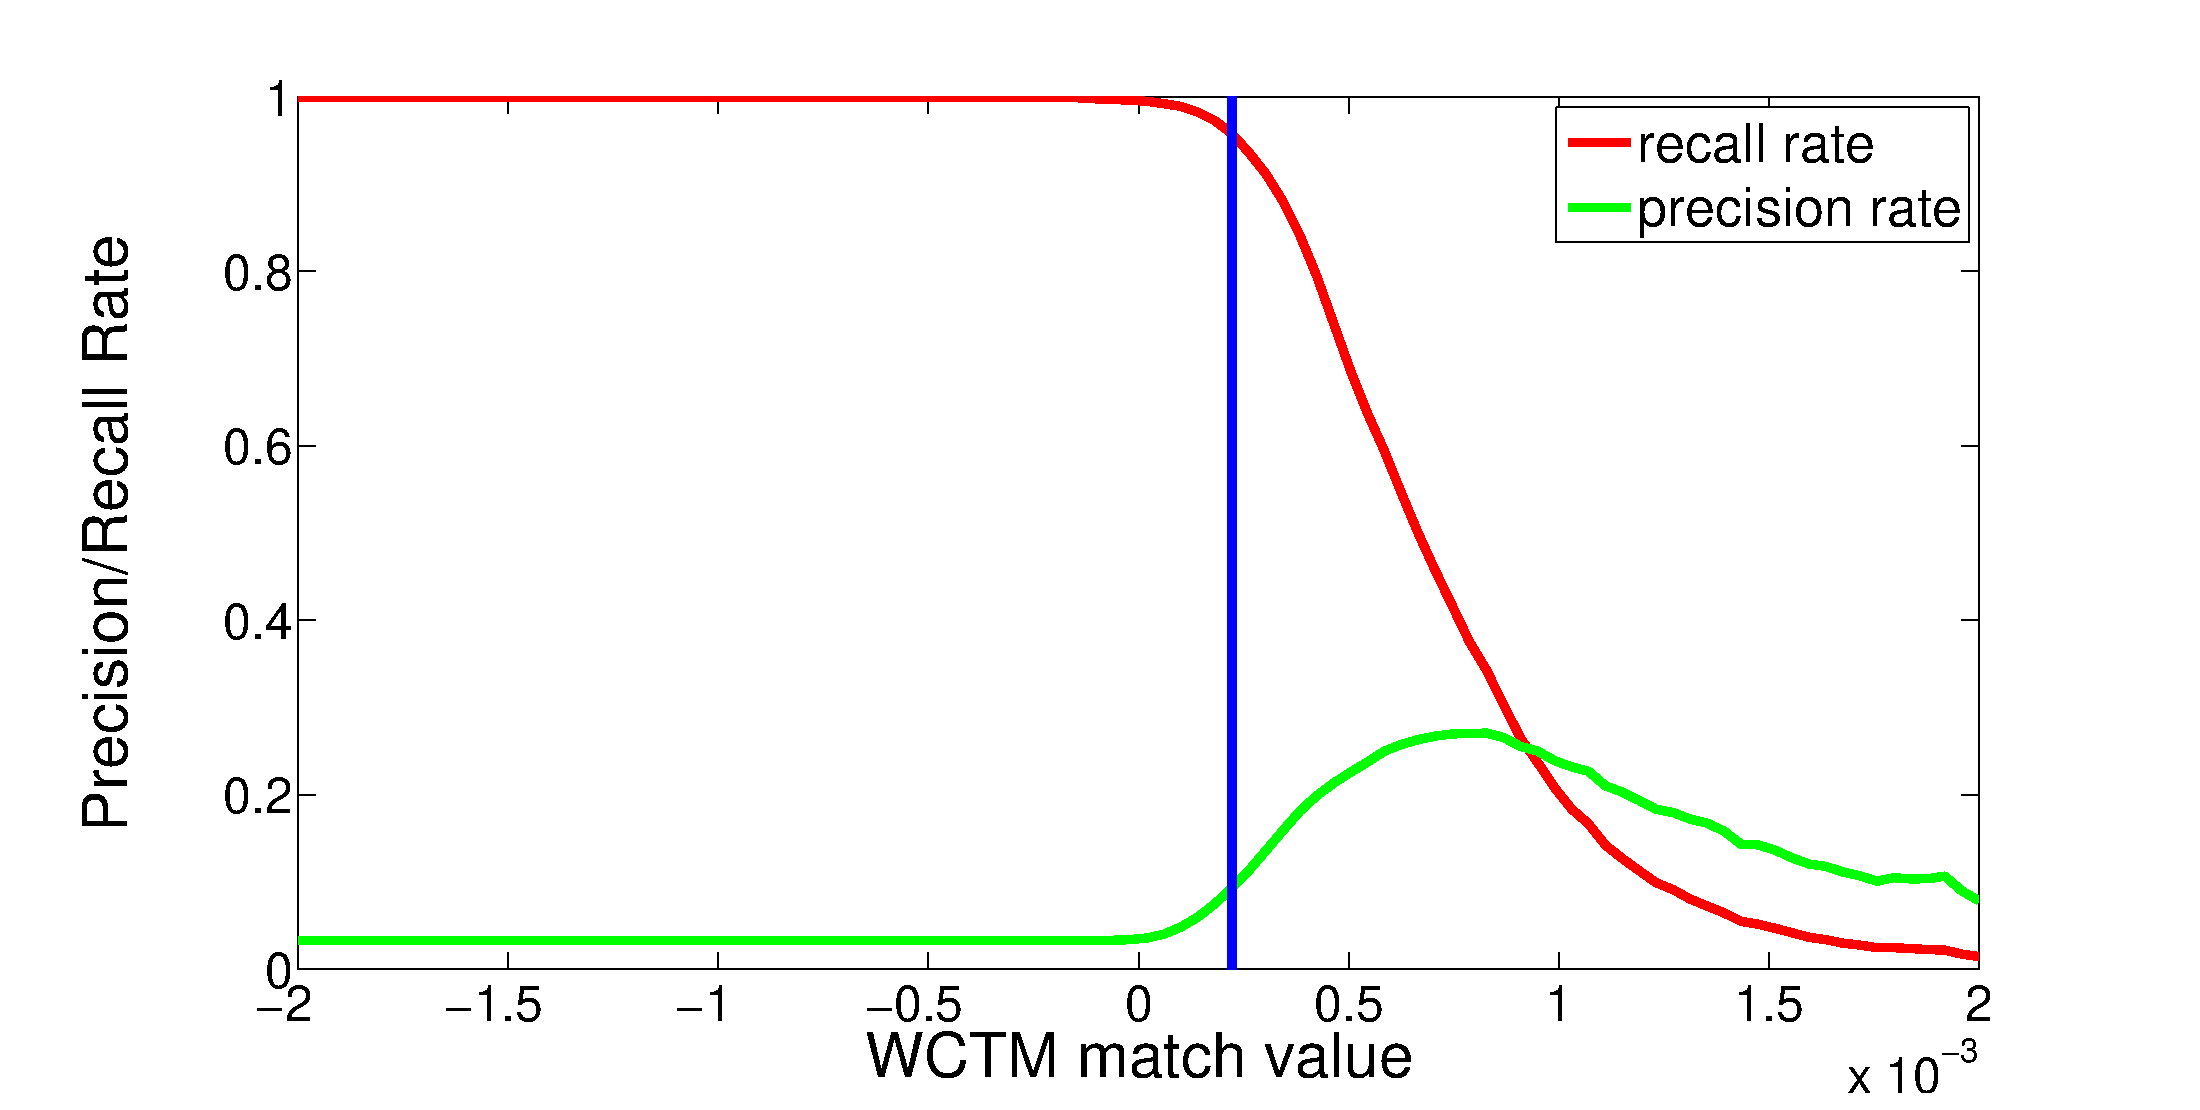
\includegraphics[width=\textwidth]{layer4_precision_recall}
      \caption{}
      \label{subfig:layer4_precision_recall}
  \end{subfigure}
  \begin{subfigure}{0.45\textwidth}
      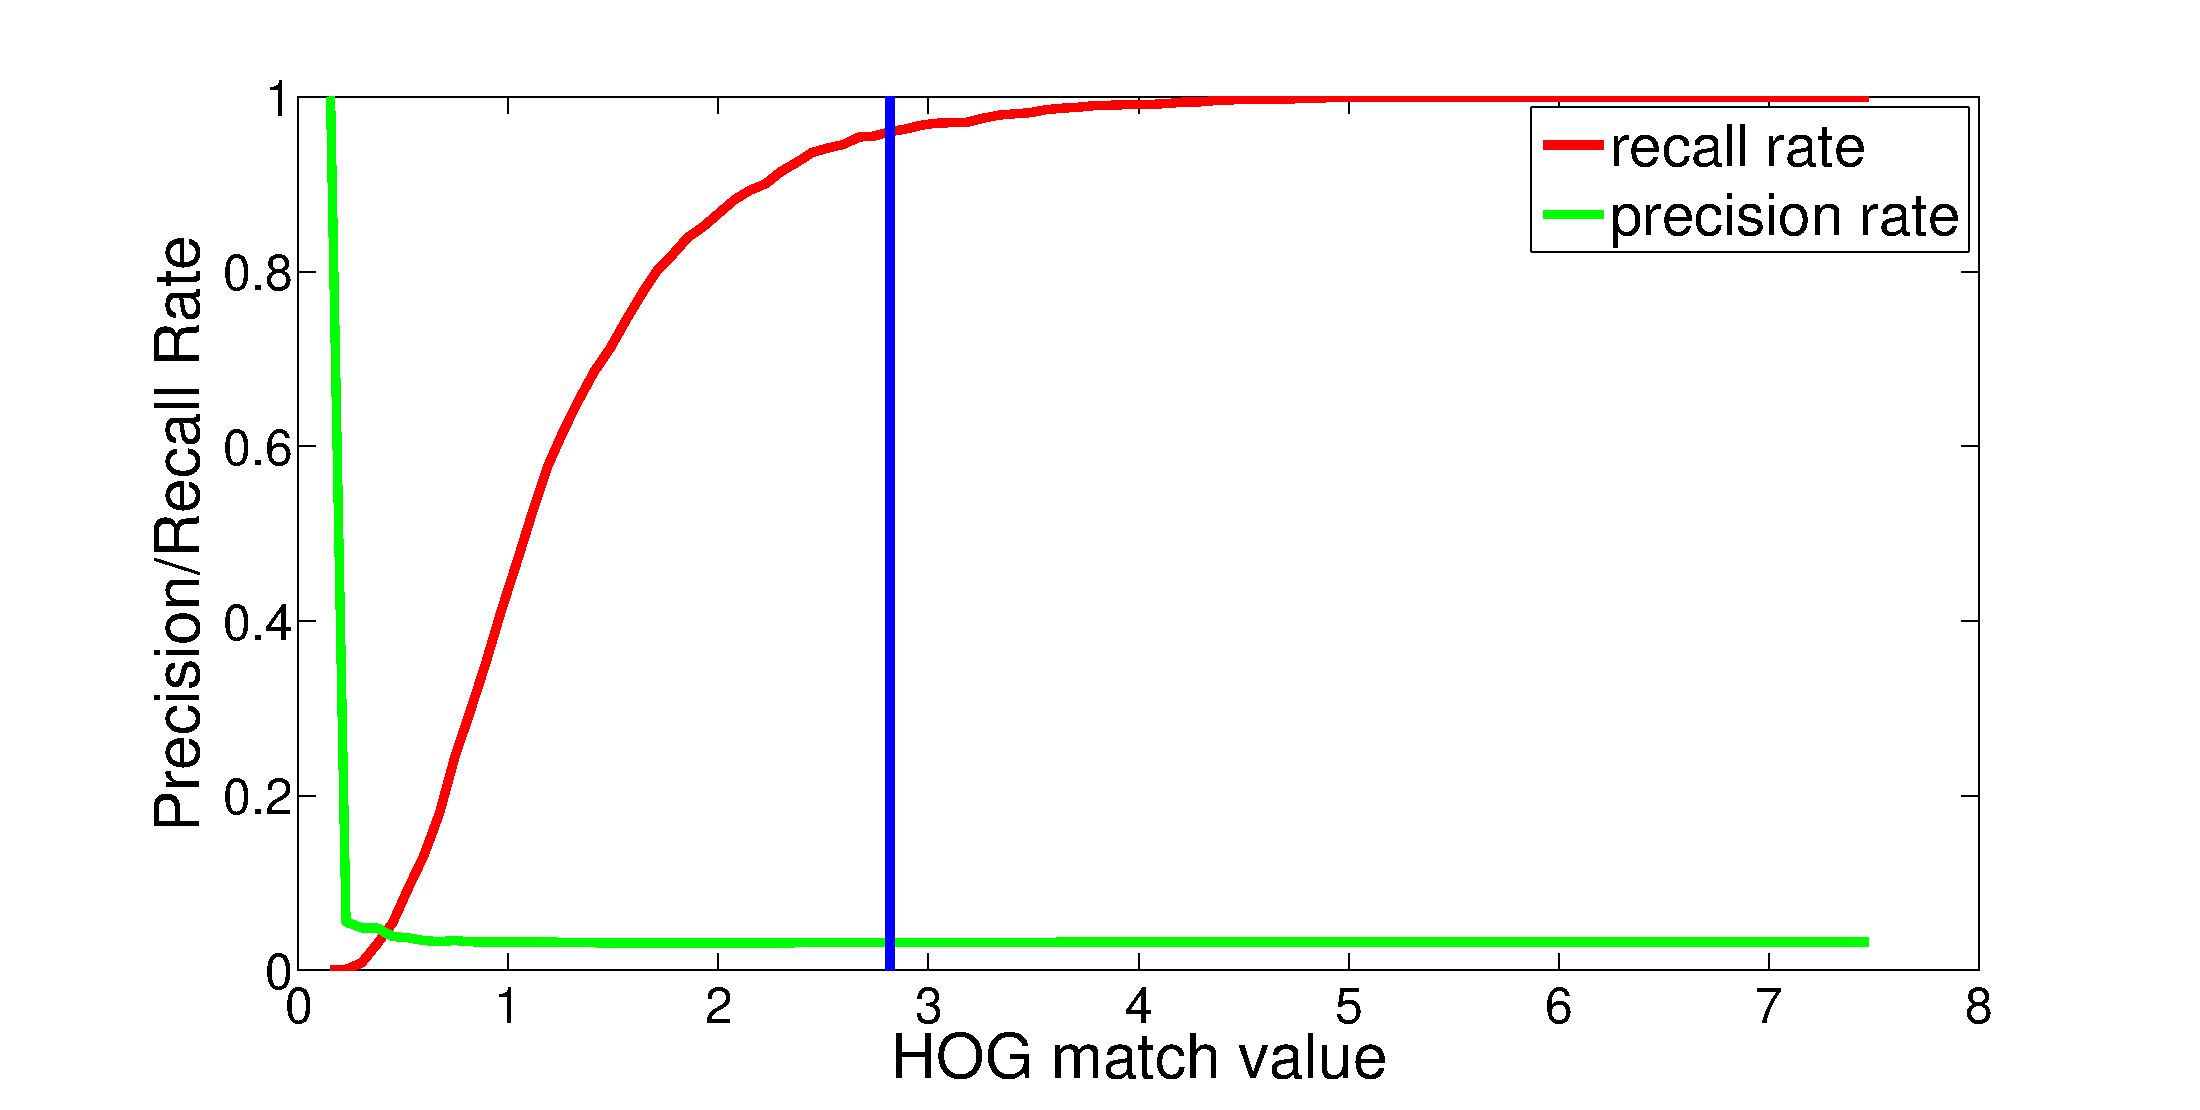
\includegraphics[width=\textwidth]{layer4_hog_precision_recall}       
      \caption{}
      \label{subfig:hog_precision_recall}
  \end{subfigure}
  \caption[Precision-Recall curves for False-positive Filtering Layer]{Precision recall curve for Layer IV candidate methods (a) \gls{wctm} and (b) \gls{hog}. The blue line marks thresholds $D_\mathsf{wctm}=0.0002222$ and $D_\mathsf{hog}=2.816$. It is important to note that \gls{wctm} is a similarity measure and \gls{hog} is a dissimilarity measure. This implies that only instances below the indicated threshold $D_\mathsf{wctm}$ in \gls{wctm}, and likewise instances above the threshold $D_\mathsf{hog}$ in \gls{hog}, are rejected as false positives. }
\end{figure}

\subsubsection{Histogram of Gradients (HOG)}
The \gls{hog} feature descriptor encodes an object by capturing a series of local gradients in neighborhood of the object pixels. 
These gradients are then transformed into a histogram after discretization and normalization. 
There are several variants of \gls{hog} feature descriptors. 
The \textsc{R-}\gls{hog} used for human detection in \cite{dalal} was tested here as a possible Layer IV candidate.

To produce \textsc{R-}\gls{hog}, the image is first tiled into a series of $8\times8$ pixel groups referred to here as cells (the image dimensions need to be multiples of 8). 
The cells are further divided into a series of overlapping blocks each containing groups of $2\times2$ cells. 
For each cell a set of 64 gradient vectors (one per pixel) is computed. 
Each gradient vector contains a direction and magnitude component. 
In the gradient directions, the sign is ignored reducing the range of angles from 0--360 down to 0--180. 
The gradient vectors are then binned into a 9--bin histogram ranging from 0--180 degrees with a bin width of 20 degrees. 
The contribution of each gradient vector is computed as half its gradient magnitude. 
The other half of the gradient magnitude is split between the two neighboring bins (in case of boundary bins, the neighbors are determined by wrapping around the histogram). 
The histograms from the 4 cells in each block is then concatenated to get vector $v$ of $36$ values ($9$ per cell). 
These vectors from each block are then normalized using their $L_2$-norm; for a vector $v$ this normalization would be expressed as
\[
 \bar{v}=\frac{v}{\sqrt{\|v\|^2_2+\epsilon^2}}
\]
where $\epsilon$ is a small constant (here $\epsilon=0.01$). 
The normalized vector $\bar{v}$ from each block is concatenated into a single feature vector $F$ to get the \gls{hog} descriptor for the input image. 
%

Since this method imposes a constraint on the image dimensions being multiples of 8, the learning samples (each cropped using a square window of size of $3\times \text{radius}$) are resized to $24\times24$. 
Here, we have to use both positive and negative object samples, the latter being objects other than scallops picked up in the segmentation layer. 
A \gls{hog} feature vector $F$ of length $144\enspace (4\enspace \text{blocks} \times4\enspace \text{cells} \times9\enspace \text{values})$ is computed for each object instance obtained from the classification layer.

Now several different machine learning methods can be applied, using the positive and negative object instances as learning samples. 
As per the original implementation of the \textsc{R-}\gls{hog} method \cite{dalal}, an \gls{svm} is used here. 
It turns out that the \gls{svm} learning algorithm fails to converge even after a large number of iterations. 
This could be attributed to the fact that the scallop profiles  vary significantly based on their position in the image. 
To overcome this limitation, a lookup table similar to the one used to learn the scallop profiles in the classification layer is generated. 
The only difference here is that instead of saving a reference scallop template vector, a reference \gls{hog} vector for only positive scallop instances from the learning set is recorded. 
The reference \gls{hog} descriptor for a pixel coordinate in the image is taken to be the mean of all the \gls{hog} descriptors of scallop instances inside a $40\times40$ window around the point.

For each instance classified as a scallop from the classification layer, its \gls{hog} descriptor is compared with its corresponding learned reference \gls{hog} descriptor from the lookup table.
Since \gls{hog} feature vectors are essentially histograms, the \gls{emd} metric \cite{rubner} is used to measure the dissimilarity between feature and object histograms.
%Technically, the \gls{emd} quantifies the difference between two histograms. Intuitively, if histogram bins are thought of as containers of dirt with the volume of dirt in each bin is analogous to the bin frequency, then the amount of work done moving piles of dirt to match a different histogram arrangement is equivalent to the \gls{emd}  between the two histograms. 
Let $A$ and $B$ be two histograms, and let $m$ and $n$ be the number of bins in $A$ and $B$, respectively.
Denote $d_{ij}$ the spatial (integer) distance between bin $i$ in $A$ and bin $j$ in $B$, and $f_{ij}$ the smaller number of items that can be moved between bins $i$ and $j$ to ultimately make both histograms match (this is known as the \emph{optimal flow} and can be found through a process of solving a linear program \cite{rubner}).
Then the \gls{emd} metric $D_\mathsf{emd}$ that quantifies dissimilarity between two histograms $A$ and $B$ would be expressed as
%
\[
 D_\mathsf{emd}(A,B)=\frac{\sum_{i=1}^m\sum_{j=1}^nd_{ij}f_{ij}}{\sum_{i=1}^m\sum_{j=1}^nf_{ij}} \enspace.
\]


A precision-recall curve (shown in Figure~\ref{subfig:hog_precision_recall}) with the classification threshold set as $2.816$ (which corresponds to 96\% recall rate, same rate used to set the \gls{wctm} threshold). 
Any object with \gls{emd} distance value less than this threshold is considered as a scallop.
 Though this threshold can capture 96\% of the scallops, very few false positives actually get eliminated (less than 3\%).

%========================================================================================
\section{Results}
%
The multi-layered detection approach is tested on two separate datasets containing  $1\,299$ and $8\,049$ images, respectively.
Among the two candidate methods tested for the fourth layer, \gls{wctm} was chosen over \gls{hog} due to it superior performance in terms of eliminating false positives. 
The difference in performance between \gls{hog} and \gls{wctm} is given in Table~\ref{tab:false_positives} for both datasets. 
Rows 1 and 2 in Table~\ref{tab:false_positives} show the true positives and false positives, respectively, that are filtered down from the initial 3 layers (Layers I-III). 
With these values as baseline, the thresholds for both \gls{hog} and \gls{wctm} were chosen to retain a high recall rate of close to 96\%. 
This ensures that very few true positives are lost and their performance is primarily assessed through the reduction in false positives (row 6 of Table~\ref{tab:false_positives}). 

\begin{table*}
  \centering
  \begin{threeparttable}
    \begin{tabular}{lllll}
\toprule[1pt]
	&\multicolumn{2}{c}{\gls{hog}}	&\multicolumn{2}{c}{\gls{wctm}}\\
	&Dataset 1	&Dataset 2	&Dataset 1	&Dataset 2\\ [2pt]\cline{1-5}\\[-5pt]
TP\tnote{1} ~from Classification Layer	&183		&1\,759		&183		&1759\\
FP\tnote{2} ~from Classification Layer	&7\,970		&52\,456		&7\,970		&52\,456\\
TP after Layer IV 			&179		&1\,689		&176		&1\,685\\
FP after Layer IV 			&7\,752		&51\,329		&2\,924		&16\,407\\
Decrease in TP after Layer IV	&4 (2.2\%)	&70 (4\%)	&7 (3.8\%)	&74(4.2\%)\\
Decrease in FP after Layer IV	&218 (2.7\%)	&1\,127 (2.1\%)	&5\,046 (63.3\%)	&36\,049 (68.7\%)\\ \bottomrule
    \end{tabular}
    \begin{tablenotes}
	  \item[1] \footnotesize{TP--True Positives}
	  \item[2] \footnotesize{FP--False Positives}
    \end{tablenotes}                                                      
  \end{threeparttable}
  \caption{Comparison of tested false positive filter layer methods}
  \label{tab:false_positives}
\end{table*}      
%
Since the thresholds are set such that the recall rate is high in both methods, the decrease in true positives is less than 5\% in both \gls{hog} and \gls{wctm}. 
However there is a significant reduction in false positives (63.3\% for dataset 1 and 68.7\% for dataset 2)  due to \gls{wctm}. 
On the other hand, the decrease in false positives is relatively small (less than 3\%) for \gls{hog}.
It is not clear at this point why the \gls{hog} filter fails to remove  false positives. 
One reason could be that the \gls{hog} filter derived from its native implementation for human detection in \cite{dalal} might need further customization and even weighting through standard deviation weights like in \gls{wctm}. 
Further study and detailed analysis is required to investigate and possibly improve its performance. 
In any case, the results support the inclusion of \gls{wctm} as the false positive filter layer in the multi-layer scallop detection and counting process pipeline.

The overall performance of the four-layer pipeline is shown in Table \ref{tab:count_results}.  
The results are compared to manually labeled ground truth.
Only a subset of the available scallops---scallops at least 80 pixels horizontally and 60 pixels vertically away from the image boundaries---were used as ground truth.
This was done to leave out scallops near the boundaries that were affected by severe vignetting effects. 
Such scallops were often too dark (see Figure~\ref{fig:scallopred}) and very difficult to correct using standard vignetting correction algorithms.
Furthermore, the scallop templates for scallops near the boundaries are such that their prime feature, the dark crescents, blend into the dark borders of the image (see Figure~\ref{subfig:mean_quadrant}). 
Inclusion of the boundaries would cause almost any objects near the boundary to be classified as scallops, resulting in a large number of false positives.
It is also interesting to note that scallops only partially visible near the image boundaries were excluded in the manual counts performed \cite{walker}.

\begin{table*}
\caption{Results of multi-layer scallop classification \label{tab:count_results}}
\begin{center}
\begin{tabular}{lll}
\toprule[1pt]
 & Dataset 1 & Dataset 2\\[2pt]\cline{1-3}\\[-5pt]
Number of images & 1,299 & 8,049\\
Ground Truth Scallops & 363 & 3,698\\
Valid Ground Truth Scallops & 250 & 2,781\\
True positives after Visual Attention Layer & 231 (92.4\%) & 2,397 (86.2\%)\\
True positives after Segmentation Layer & 185 (74\%) & 1,807 (64\%)\\
True positives after Classification Layer & 183 (73\%) & 1,759 (63.2\%)\\
True positives after False Positive Filter Layer & 176 (70.4\%) & 1,685 (60.6\%)\\
False positives after Classification Layer & 7,970 & 52,456\\
False positives after False Positives Filter Layer (\gls{wctm}) & 2,924 & 16,407\\
Decrease in false positives (due to \gls{wctm}) & 63.3\% & 68.7\%\\ \bottomrule
                               \end{tabular}
                               \end{center}
                               \end{table*}      
   
Table \ref{tab:count_results} shows the results of the 3-layer pipeline along with the improvements in terms of the reduction in false positives as a result of introducing the fourth processing layer. 
The true positive percentages shown are computed with reference to the valid ground truth scallops (row 3 of table \ref{tab:count_results}), i.e., scallops away from image boundaries.  
In dataset 1, which contains $1\,299$ images, the four-layer filtering results in a 70.4\% overall recall rate, while in dataset 2 that contains $8\,049$ images the overall recall rate is 60.6\%.  Though the addition of the fourth false positive layer results in a small drop of 2.6\% in recall rate, it eliminates over 63\% of the false positives in both datasets.
There is no clear reason for the better performance of this pipeline on dataset 2 both in terms of recall rate and decrease in false positives compared to dataset 1.

%========================================================================================
\section{Discussion}
\label{sec:scallop_discussion}

The four-layer automated scallop detection approach discussed
here works on feature-poor, low-light imagery and yields
overall detection rates in the range of 60--70\%. 
Related work on scallop detection using underwater imaging \cite{dawkins11,dawkings13},
reported higher detection rates, but the quality of the images used was visibly better.  Specifically,
the datasets on which the 
alternative algorithms \cite{dawkings13}
operated on, exhibit much more uniform lighting conditions, higher resolution,
brightness, contrast, and color variance between scallops and background 
(see Figure~\ref{data-difference}). 
Evidence of this can be seen in Figure~\ref{data-difference}: the color variation between scallops and background data is reflected in the
saturation histogram of Figure~\ref{data-difference}. While the histograms
of scallop regions in the datasets of Table~\ref{tab:count_results} is often 
identical to the global histogram of the image, the histograms of the \gls{whoi} data used by the alternative algorithms \cite{dawkings13} present a bimodal saturation histogram
(Figure \ref{subfig:dawkins_hist}), from which 
foreground and background are easily separable.



\begin{figure*}
  \centering
  \begin{minipage}[c]{\textwidth}
    \centering
    \raisebox{1.5mm}{
    \begin{subfigure}[]{0.3\textwidth}
	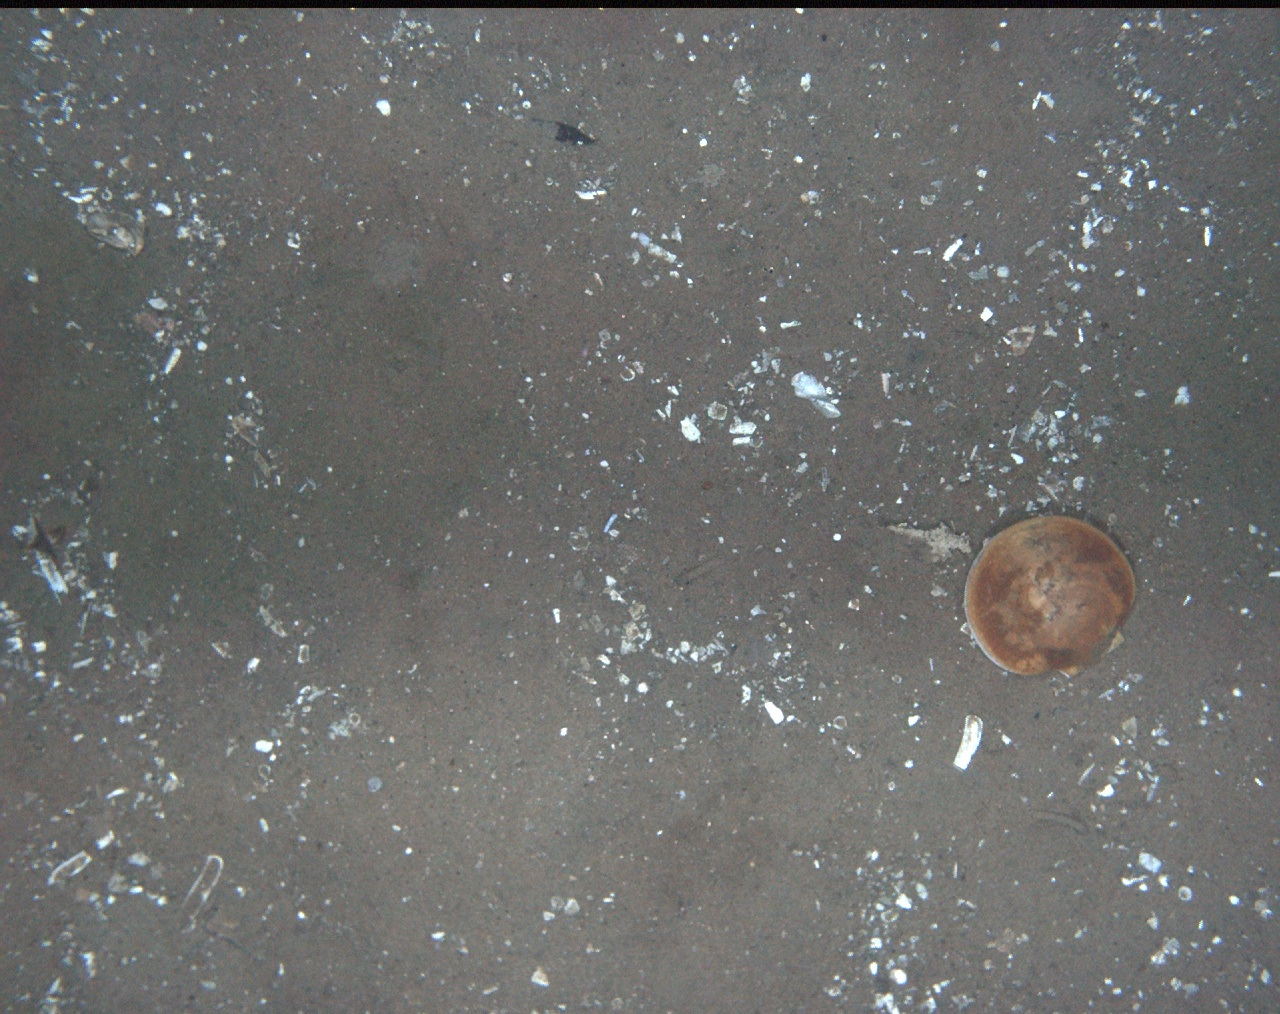
\includegraphics[width=\textwidth,natwidth=1280,natheight=1014]{77616}
	\caption{}
	\label{subfig:dawkins}
    \end{subfigure}
    }
    \begin{subfigure}[]{0.25\textwidth}
	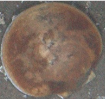
\includegraphics[width=\textwidth,natwidth=105,natheight=100]{dawkins_crop_resize}
	\caption{}
	\label{subfig:dawkins_crop}
	\hskip 15pt
    \end{subfigure}
    \raisebox{2mm}{
    \begin{subfigure}[]{0.33\textwidth}
	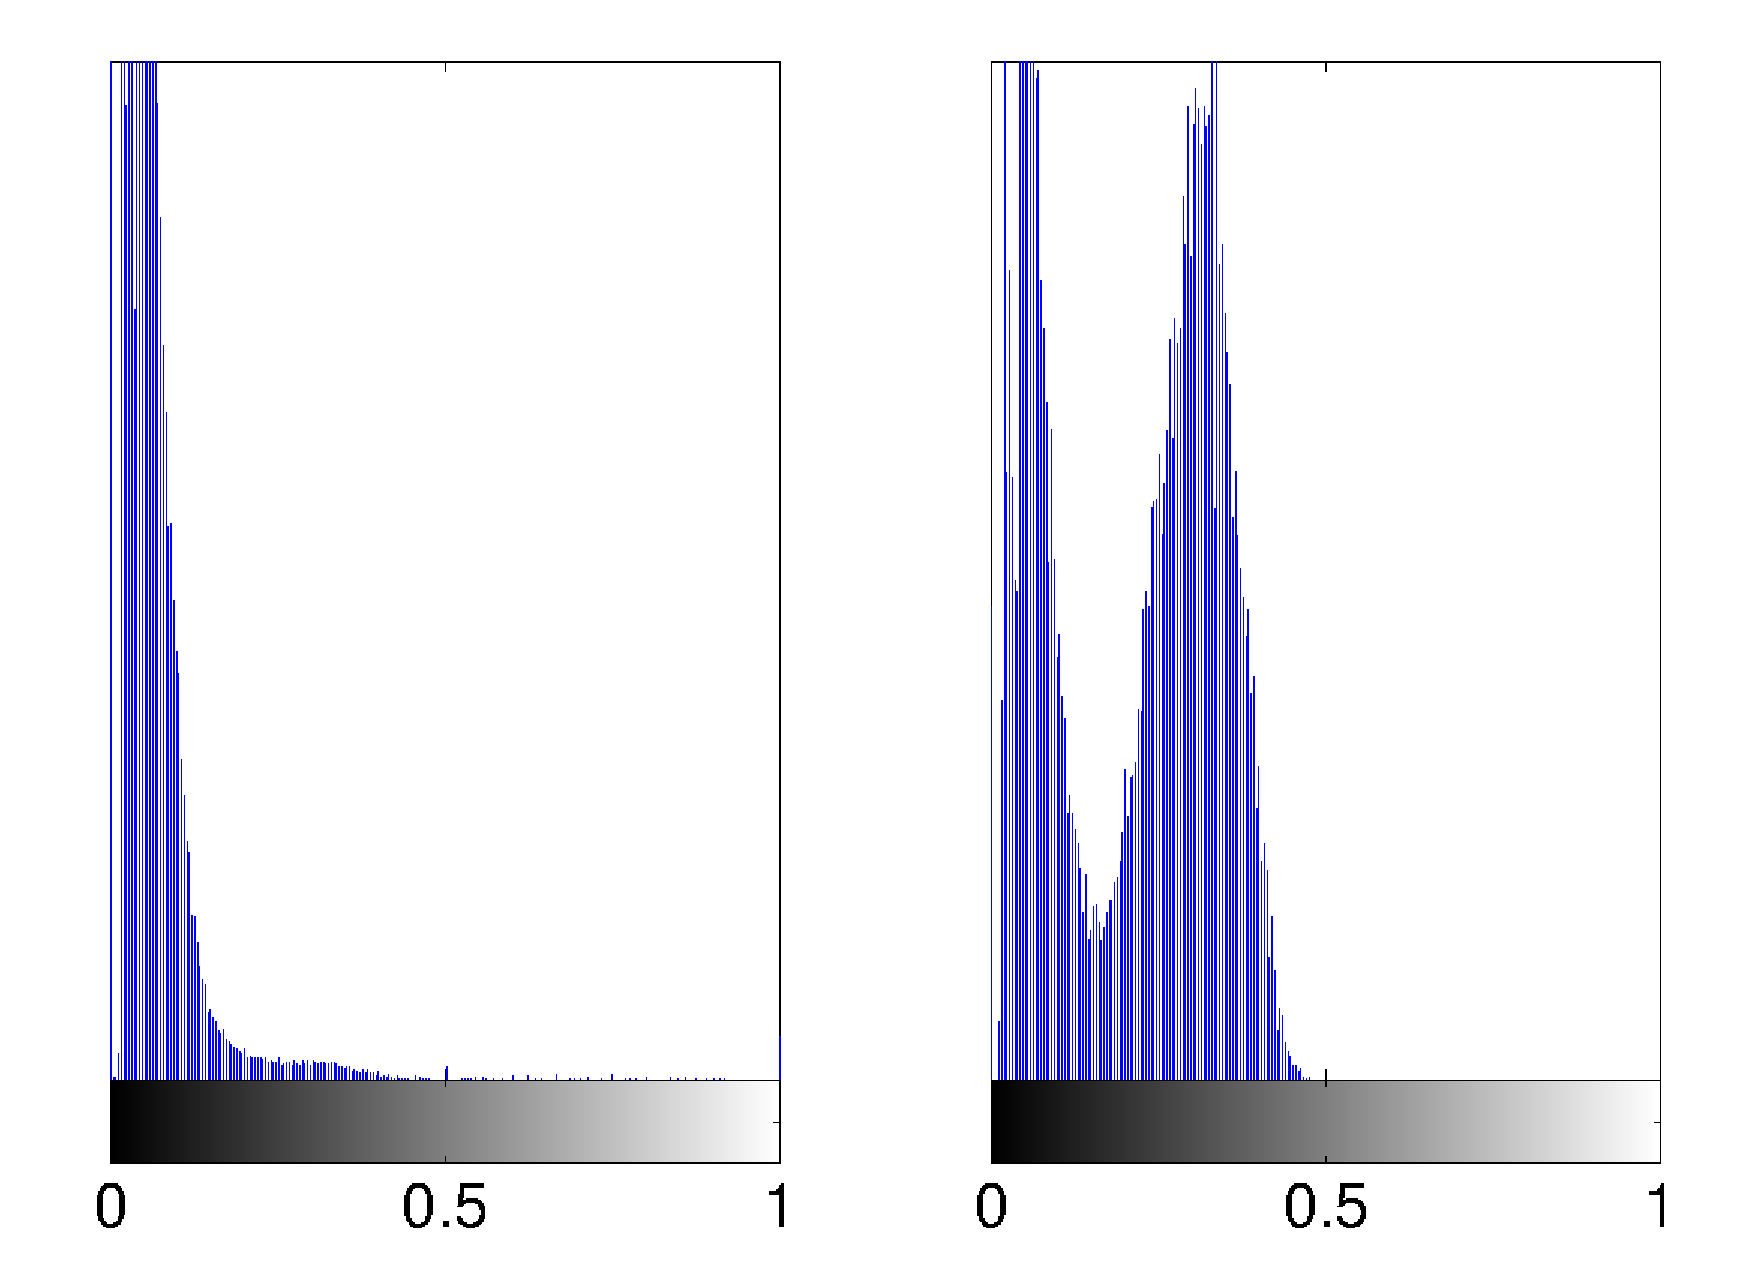
\includegraphics[width=\textwidth]{dawkins_hist_sat}
	\caption{}
	\label{subfig:dawkins_hist}
    \end{subfigure}
    }
  \end{minipage} 

  \vskip 10pt
  \begin{minipage}[c]{\textwidth}
  \centering
    \raisebox{1.5mm}{
    \begin{subfigure}[]{0.32\textwidth}
	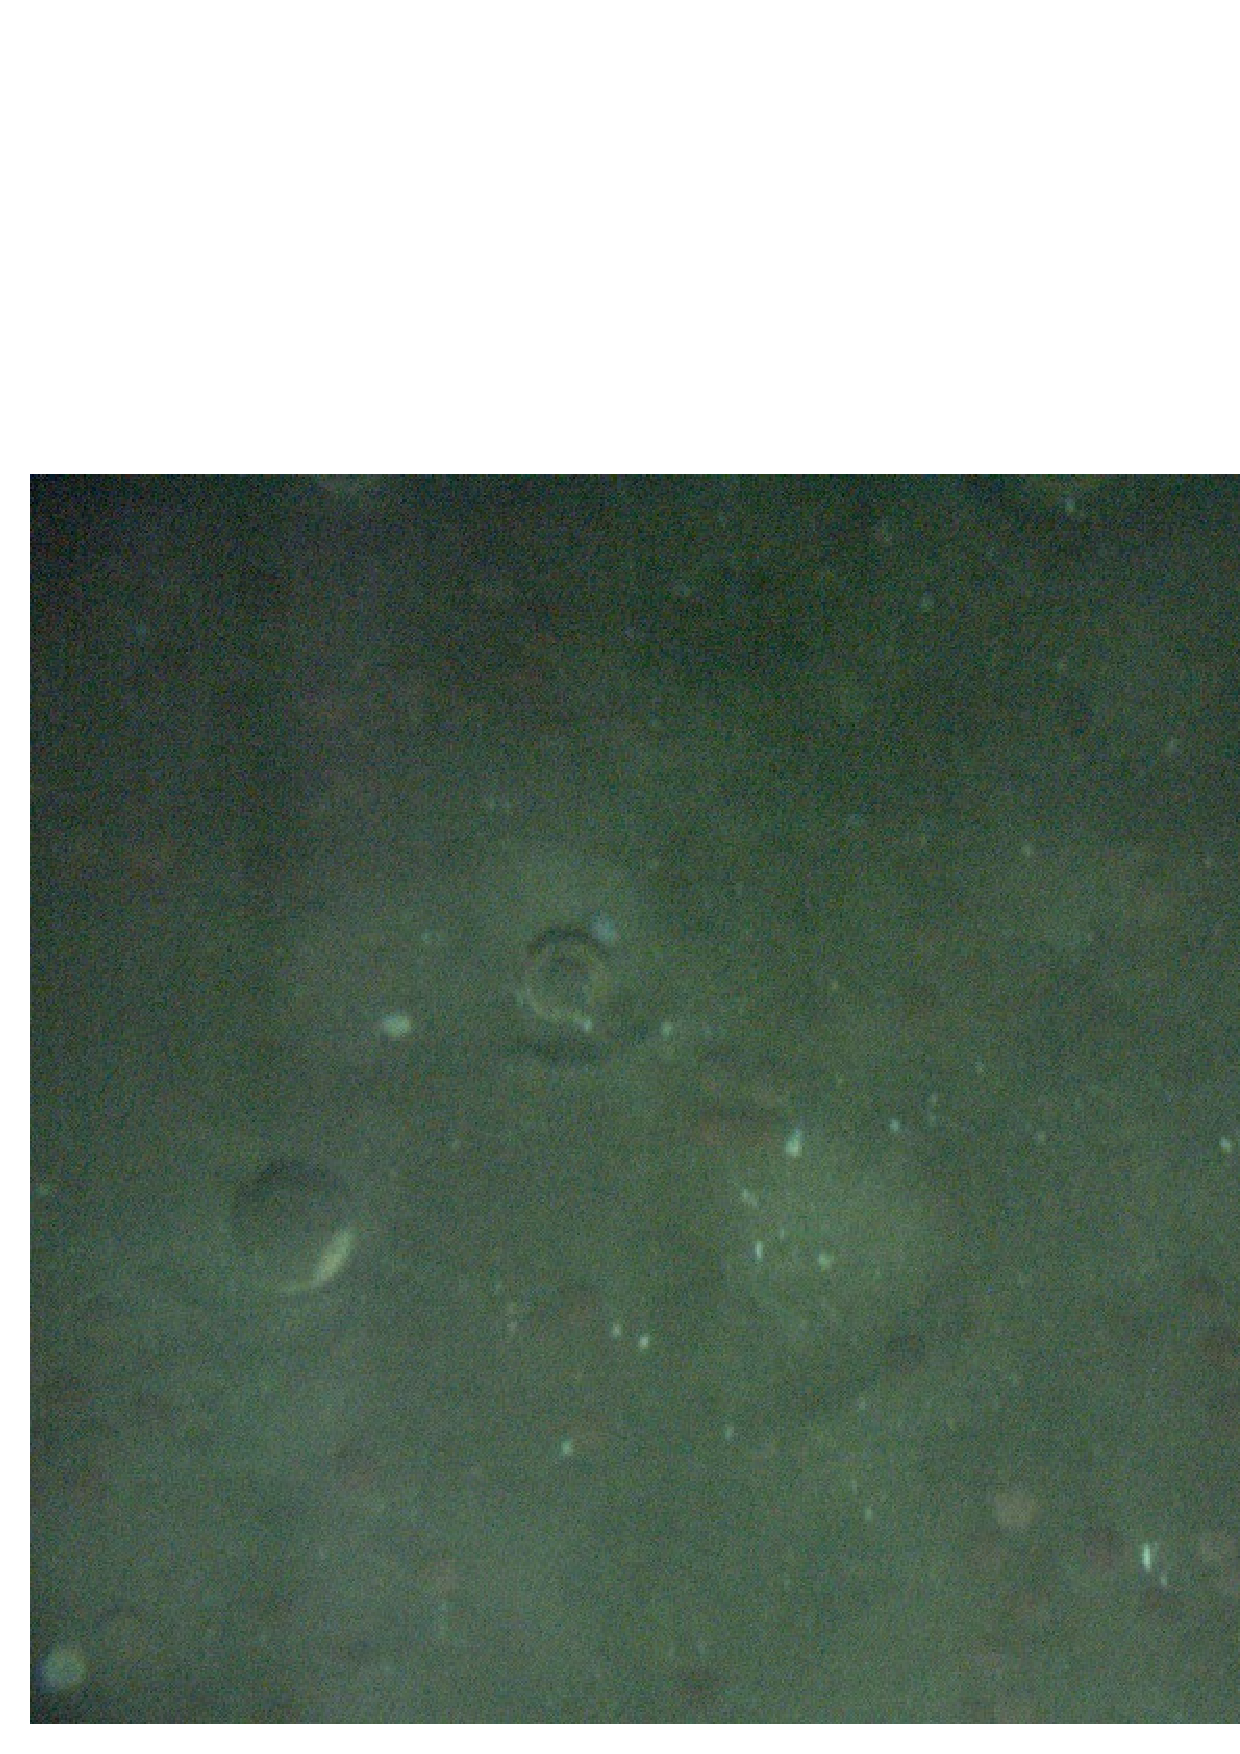
\includegraphics[width=\textwidth]{60} 
  	\caption{}
	\label{subfig:typical}
    \end{subfigure}
    }
    \begin{subfigure}[]{0.235\textwidth}
	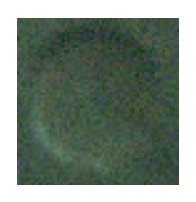
\includegraphics[width=\textwidth]{our_crop_resize}
	\caption{}
	\label{subfig:typical_crop}
	\hskip 15pt
    \end{subfigure}
    \raisebox{2mm}{
    \begin{subfigure}[]{0.35\textwidth}
	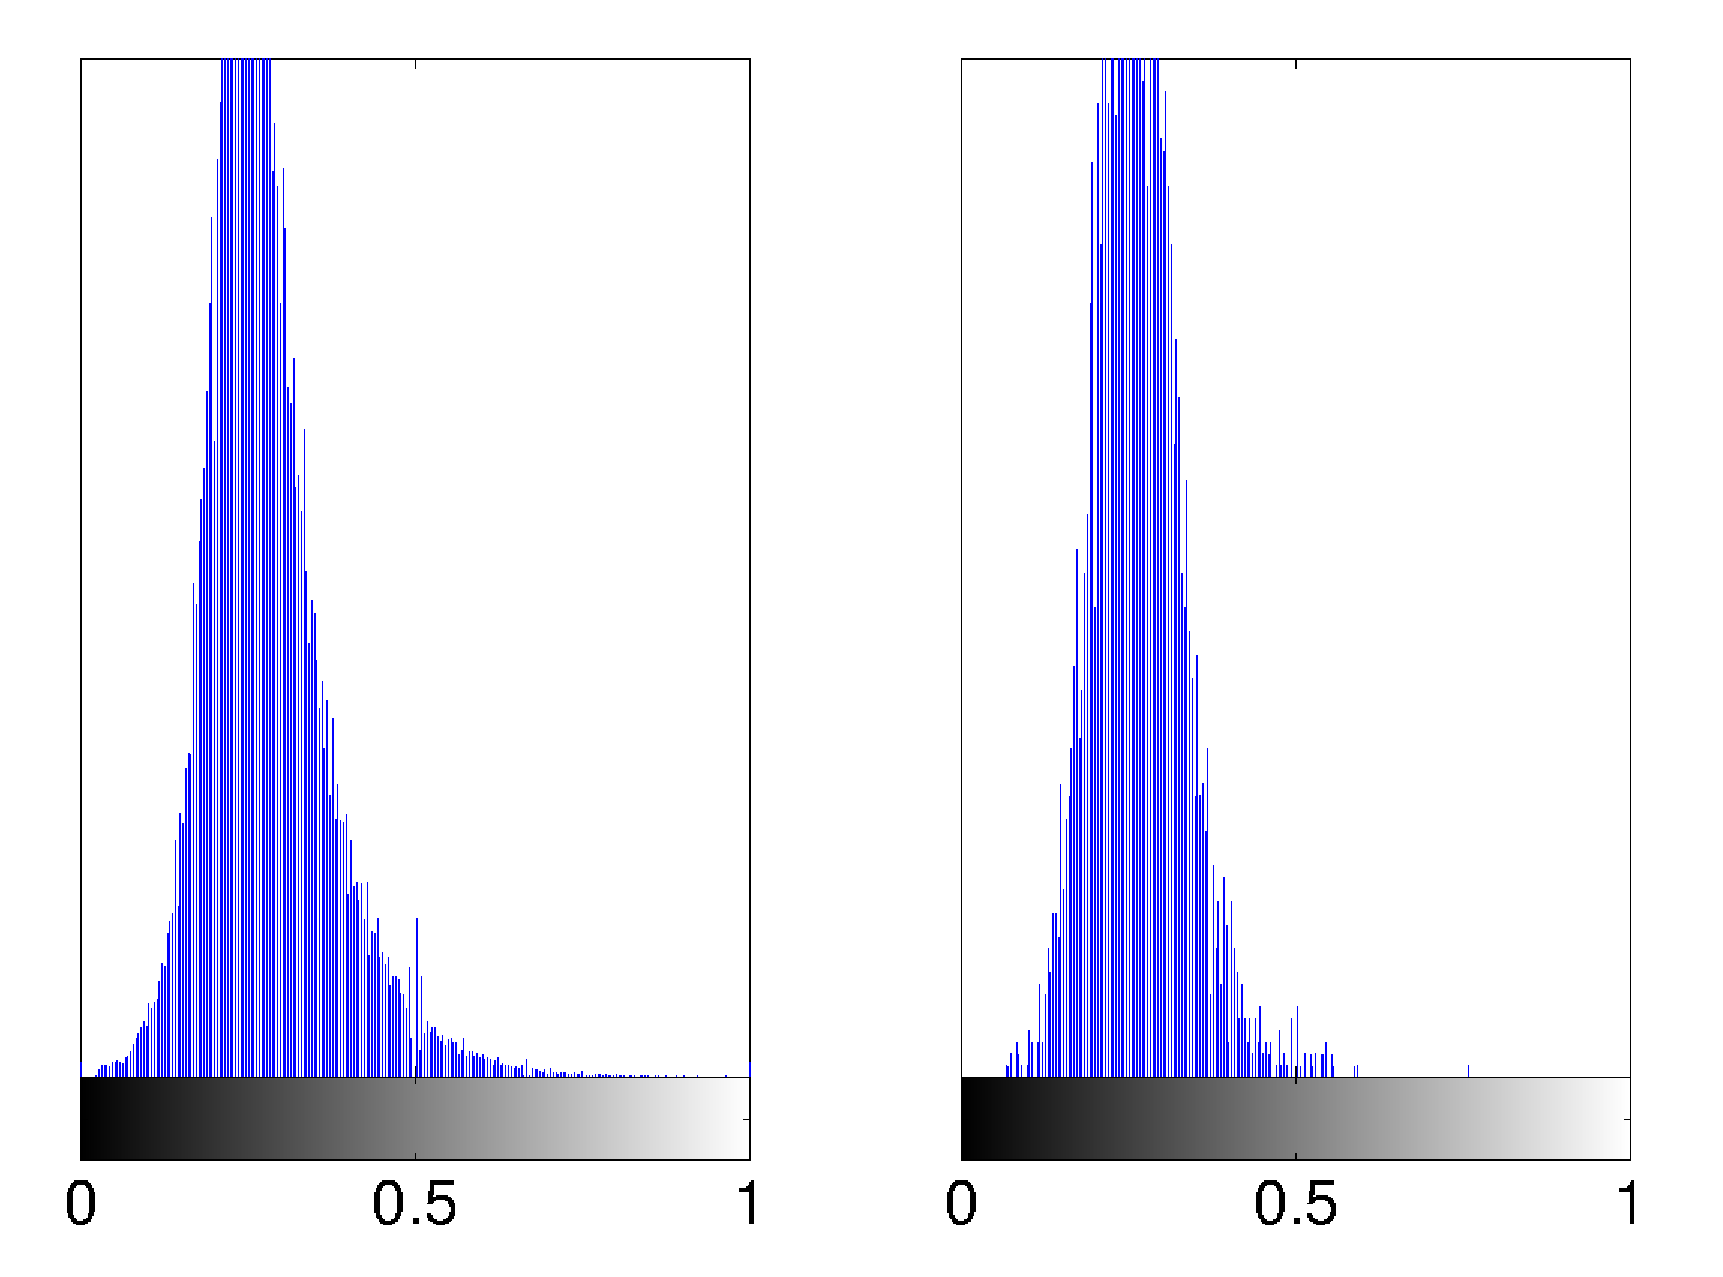
\includegraphics[width=\textwidth]{our_hist_sat}
	\caption{}
	\label{subfig:typical_hist}
    \end{subfigure}
    }
  \end{minipage}
  \caption[Comparison of scallop recognition results with existing methods]{Representative samples of different imagery data on which
  scallop detection algorithms may be called to operate on.  Figures \ref{subfig:dawkins}
  and \ref{subfig:typical},
  show an image containing a single scallop from the dataset used by Dawkins et al.\cite{dawkings13} (used with permission from the authors) 
  and the datasets used in this chapter respectively.
  A magnified
  view of a scallop cropped from Figure \ref{subfig:dawkins} 
  and \ref{subfig:typical} can be seen in Figures \ref{subfig:dawkins_crop} 
  and \ref{subfig:typical_crop} respectively.
  Figure \ref{subfig:dawkins_hist} 
  gives the saturation histogram of background or the complete 
  image in Figure \ref{subfig:dawkins} to left and 
  saturation histogram of Figure \ref{subfig:dawkins_crop} to the right.
  Similarly, Figure \ref{subfig:typical_hist} 
  gives the saturation histogram of Figure \ref{subfig:typical} to the left and 
  saturation histogram of Figure \ref{subfig:typical_crop} to the right. The bimodal 
  nature of the scallop histogram
  in Figure~\ref{subfig:dawkins_hist} 
  derived from the dataset used in Dawkins et al.\cite{dawkings13}, clearly portrays the distinguishing appearance of the scallop pixels from the rest of the image, making it easily identifiable. The datasets we
  used did not exhibit any such characteristics (as seen in Figure~\ref{subfig:typical_hist}) 
  to aid the identification of scallops.}
  \label{data-difference} 
\end{figure*}

Compared to another alternative approach that uses a series of bounding boxes to cover the entire image \cite{guomundsson}, the one reported here employs only ten windows per image, scanning the images at a much faster rate.   
Additionally, the detection rates there \cite{guomundsson} were based on a dataset of just 20 images; statistically significant differences in performance rates between that approach and the one reported here would need much larger image samples.

%========================================================================================
\section{Conclusions}

With the increasing use of underwater robotic platforms, terrabytes of imagery datasets featuring millions of images is becoming increasingly common. 
The current practice of manual processing of these underwater images introduces a bottleneck. 
In the spirit of this scallop counting work, designing better and faster automated tools  to characterize animals and other natural underwater phenomenon from images is imperative for future marine environmental studies.

This work is a step toward
the development of an automated procedure for scallop detection, classification
and counting, based on low-resolution imagery data obtained in the organisms' natural environment.
The uniqueness of the reported method lies in its ability to handle poor lighting and low-contrast imaging conditions.
A large natural datasets of over 8000 images have been used to validate this four-layered framework.
Augmenting a previously developed three-layer scallop counting framework with a dedicated false-positive filtering layer has a drastic effect in terms of reducing the number of false positives.
The study noted that a filter based on a custom \gls{wctm} method outperforms \gls{hog} in  this specific application context. 
The multilayer framework reported is verified to be modular, and it allows easy adaptation of different layers for various applications like counting other sea organisms. 
Designing such tools with further improvements in form of higher detection rates and lower false positives is required to help advance future marine animal studies.

%========================================================================================
\section{Future Work}

To further this analysis and reduce false positives, the false positives filter layer can be enhanced by using multiple scallop reference templates for each pixel location. 
These new templates could be designed to capture the bright crescents that sometimes appear due to the visible interior of the lower valve of a scallop when the scallop shell is partly open. As this crescent appearance is only dependent on the relative scallop orientation with respect to the camera, it can occur at any point in the periphery of a scallop. If these bright crescents were to be used in conjunction with dark crescents multiple templates will be required to model scallops at each pixel location.
This idea is supported by inspection of recently collected high-resolution scallop data, which indicate additional definitive features connecting the position of the bright and dark crescents along with their relative intensities. 
We believe that even without major changes to the current framework, testing on higher resolution images could produce much better performance outcomes (both in terms of detection and false positive rates). 
The unavailability of ground truth for the new datasets makes it hard to provide evidence of any performance at this point. 
It is also expected that using more targeted color and light correction methods \cite{dawkings13} as a part of image preprocessing will improve results.

Though this multi-layered algorithm works decently well, there is still scope for building a more robust object classification technique that is capable of handling noisy data.
Building robust object classification techniques capable of handling noisy data, is one of the primary directions where improvement is necessary. 
It may also be the case that a single noisy image of a target object might lack the information needed to accurately recognize it. With this in mind, a multi-view object recognition approach that combines information from multiple images is proposed in Chapter~\ref{chap:distdes}.

%========================================================================================

\printglossary[type=\acronymtype]                  
%
% This is the Bibliography file (bibtex.tex)
% This generally works for BibTeX

% Use sample.bib for BibTeX database
\bibliography{thesis_ref}
% BibTeX style (plain, alpha, unsrt)
\bibliographystyle{plain}
   % This file (bibtex.tex) contains the text
                   % for a bibliography if using BibTeX with
                   % sample.bib
\end{document}


